\chapter{Sample Selections and Systematics}
\label{chap:SelsAndSysts}

The oscillation analysis presented within this thesis is built upon a simultaneous fit to atmospheric data at SK, neutrino beam data in the near detector, and beam data measured at SK. This is the first simiultaneous oscillation analysis of beam and atmospheric samples supported by the T2K and SK collaborations. Notably, the author of this thesis has been responsible for the building and developing the \texttt{MaCh3} framework to support all sets of samples simultaneously. The definitions of the samples are documented in \autoref{sec:SelsAndSysts_Sels_Atms}, \autoref{sec:SelsAndSysts_Sels_ND}, and \autoref{sec:SelsAndSysts_Sels_FD}, respectively. The data collected and used within this analysis is detailed in \autoref{tab:SelsAndSysts_Sels_DataTotal}. The near and far detector data corresponds to T2K runs 2-9 and runs 1-10, respectively. The accumulated POT and beam power for runs \quickmath{1-10} are illustrated in \autoref{fig:SelsAndSysts_Beam_PowerAndPOT}.

\begin{table}[ht!]
    \centering
    \begin{tabular}{l|c}
      \hline
      Data Type & Total \\
      \hline
      Near Detector FHC & \quickmath{1.15 \times 10^{21}}POT \\
      Near Detector RHC & \quickmath{8.34 \times 10^{20}}POT \\
      Far Detector FHC & \quickmath{1.97 \times 10^{21}}POT \\
      Far Detector RHC & \quickmath{1.63 \times 10^{21}}POT \\
      Atmospheric SK-IV & \quickmath{3244.4} days \\
      \hline
      \hline
    \end{tabular}
    \caption{The amount of data collected in each detector used within this analysis. The data collected at the near and far detector, for both neutrino beam (FHC) and antineutrino beam (RHC), is measured as the number of protons on target (POT).}
    \label{tab:SelsAndSysts_Sels_DataTotal}
\end{table}

The difference in POT recorded at the near and far detector is due to the difference in downtime. The SK detector is very stable with almost \quickmath{100\%} of data recorded during beam operation. Due to various technical and operational issues, the downtime of the near detector is significantly higher due to its more complex design and operating requirements.

The systematic parameters invoked within the flux, detector, and interaction models used within this analysis are documented in \autoref{sec:SelsAndSysts_Systs}. The standard configuration of the joint beam and atmospheric data fit utilises far detector systematics provided in the official inputs from the two experiments. Additionally, a correlated detector model which fits the parameters used in sample selections to data has been developed and documented in \autoref{sec:SelsAndSysts_Systs_FD}.

\begin{figure}[h]
  \begin{subfigure}[t]{\textwidth}
    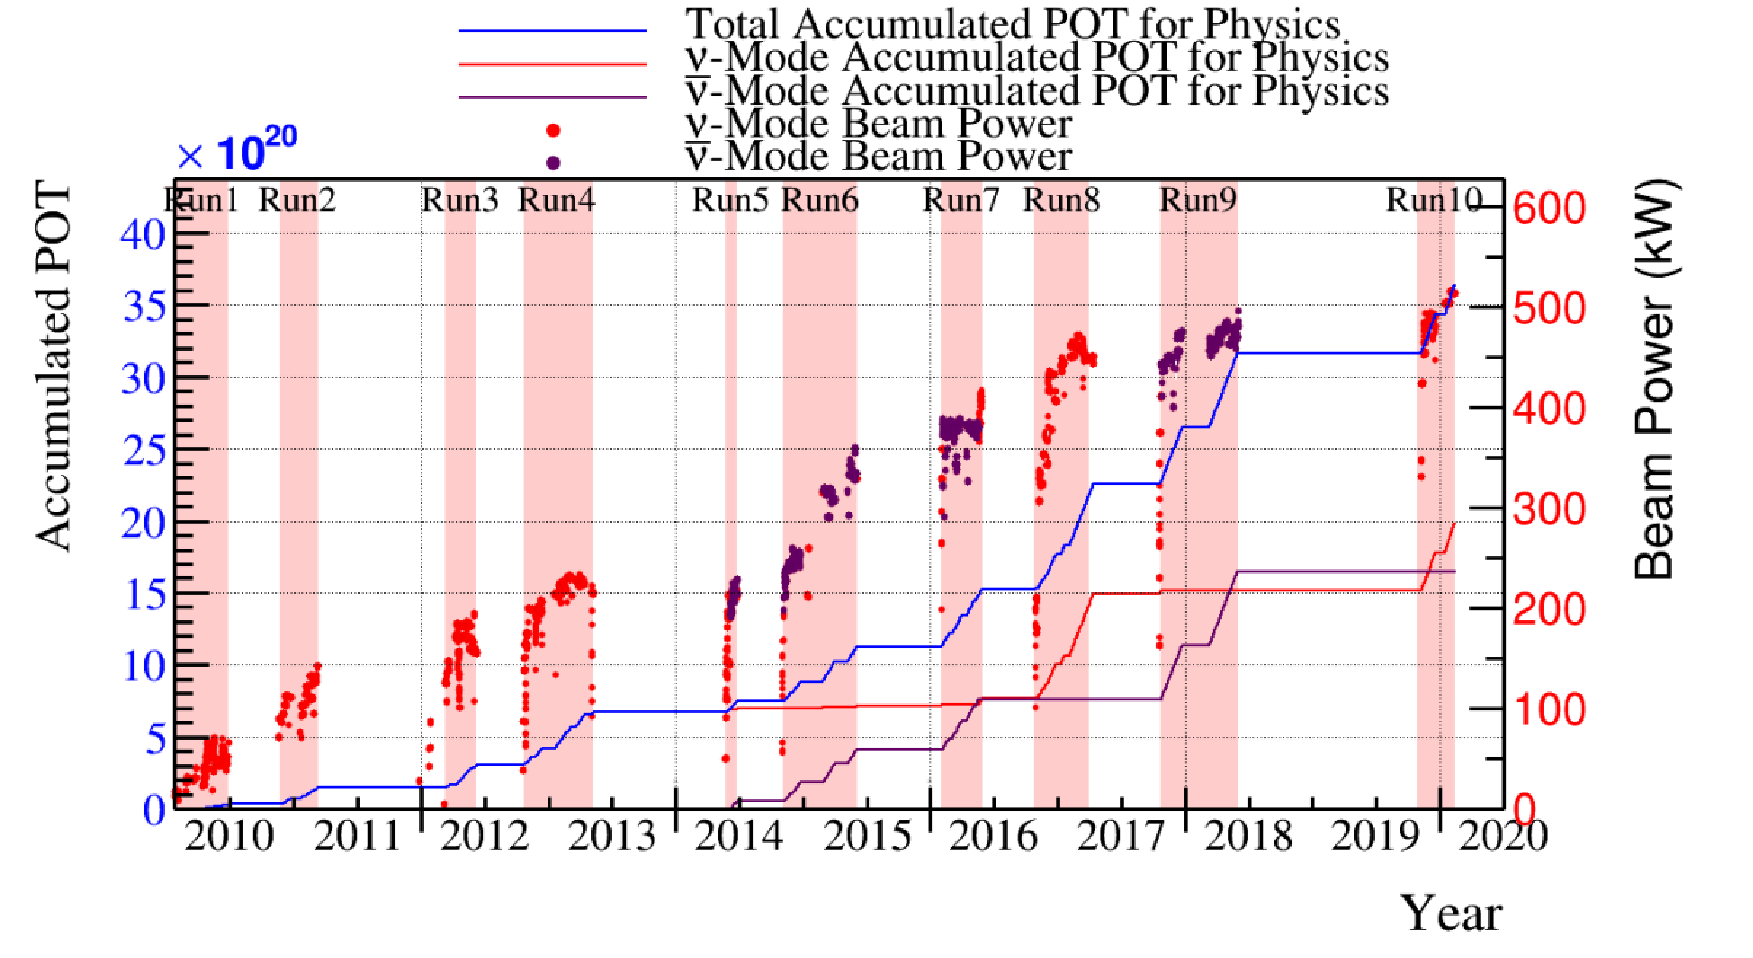
\includegraphics[width=\textwidth, trim={0mm 0mm 0mm 0mm}, clip,page=1]{Figures/Selections/BeamPowerAndPOT.pdf}
  \end{subfigure}
  \caption{The accumulated beam data, measured as the number of protons on target (POT). The total data (blue) is given which comprises of the neutrino beam (red) and antineutrino (purple) components. The beam power for neutrino and antineutrino beams is given as the markers using the same colour scheme. The timescale runs from Run 1 which started in January 2010 until Run 10 which ended in February 2020. The ratio of accumulated data in neutrino and antineutrino beam is \quickmath{54.7\%:45.3\%}.}
  \label{fig:SelsAndSysts_Beam_PowerAndPOT}
\end{figure}

\newpage
\section{Atmospheric Samples}
\label{sec:SelsAndSysts_Sels_Atms}

The atmospheric event selection follows the official SK-IV analysis presented in \cite{Jiang2019-iw} and is documented below. The Monte Carlo prediction used within this analysis corresponds to \quickmath{500} years worth of neutrino events, which is scaled down to match the SK-IV livetime of \quickmath{3244.4} days.

The fully contained (FC), partially contained (PC), and upward going muon events (up-\quickmath{\mu}) which pass the reduction cuts discussed in \autoref{sec:Simulations_Reduction} are further broken down into different samples based on reconstruction information. This section details the samples used within this oscillation analysis, alongside the chosen binning.

FC events are first separated by the visible energy deposited within the detector. This is calculated as the sum of the reconstructed kinetic energy above the Cherenkov threshold for all rings present in the event. Events are separated by whether they were above or below \quickmath{E_{vis} = 1.33\text{GeV}}. This separates ``subGeV'' and ``multiGeV'' events. Typically, lower energy events consist of charged current quasi-elastic (CCQE) interactions which are better understood and simpler to reconstruct resulting in smaller systematic uncertainties. Events are further separated by the number of rings associated with the event due to similar reasoning. As the oscillation probability is dependant upon the flavour of neutrino, electron and muon events are separated using a similar likelihood method to that discussed in \autoref{sec:Simulation_Reconstruction}. To reduce computational resources required for the reconstruction, only electron and pion hypotheses are considered so this separation cut depends on the ratio of the electron to pion likelihoods, \quickmath{\log(L_{e}/L_{\pi})}. Finally, the number of decay electrons is used to classify events. Charged current resonant pion production (CCRES) interactions generate a final-state pion. This can decay, mostly likely through a muon, into a decay electron. Therefore any electron-like event with one decay electron or muon-like event with two decay electrons was most likely produced by a CCRES interaction. Consequently, the number of decay electrons can be used to distinguish CCQE and CCRES interaction modes. Ultimately, FC subGeV events are separated into the samples listed in \autoref{tab:SelsAndSysts_Sels_Atms_SubGeV}.

\begin{table}[ht!]
    \centering
    \begin{tabular}{c|l}
      \hline
      Sample Name & Description \\
      \hline
      \texttt{SubGeV-elike-0dcy} & Single ring \quickmath{e}-like events with zero decay electrons \\ \hline
      \texttt{SubGeV-elike-1dcy} & Single ring \quickmath{e}-like events with one or more decay electrons \\ \hline
      \texttt{SubGeV-mulike-0dcy} & Single ring \quickmath{\mu}-like events with zero decay electrons \\ \hline
      \texttt{SubGeV-mulike-1dcy} & Single ring \quickmath{\mu}-like events with one decay electrons \\ \hline
      \texttt{SubGeV-mulike-2dcy} & Single ring \quickmath{\mu}-like events with two or more decay electrons \\ \hline
      \texttt{SubGeV-pi0like} & Two \quickmath{e}-like ring events with zero decay electrons \\
      & \hspace{0.2cm} and reconstructed \quickmath{\pi^{0}} mass \quickmath{85 \leq m_{\pi^{0}} < 215 \text{MeV}} \\
      \hline
      \hline
    \end{tabular}
    \caption{The fully contained subGeV samples, defined as events with visible energy\quickmath{E_{vis} < 1.33\text{GeV}}, used within this oscillation analysis.}
    \label{tab:SelsAndSysts_Sels_Atms_SubGeV}
\end{table}

In addition to the cuts discussed above, multiGeV samples also have additional cuts to separate samples which target neutrino and antineutrino events. As discussed in \autoref{sec:Oscillation_Overview}, the matter resonance only occurs for neutrinos in  the normal hierarchy and antineutrinos in the inverted mass hierarchy. Therefore, having flavour-enriched samples aids in the determination of the mass hierarchy. For a CCRES interaction,

\begin{align}
  \begin{split}
    \bar{\nu}_e + N \rightarrow e^{+} + N^{'} + &\pi^{-}, \\
    \nu_e + N \rightarrow e^{-} + N^{'} + &\pi^{+} \\
    &\hspace{5pt} \rotatebox[origin=c]{180}{$\Lsh$} \hspace{5pt} \mu^{+} + \nu_\mu \\
    &\hspace{20pt} \rotatebox[origin=c]{180}{$\Lsh$} \hspace{5pt} e^{+} + \nu_e + \bar{\nu}_\mu.
\end{split}
\end{align}

The \quickmath{\pi^{-}} emitted from a \quickmath{\bar{\nu_{e}}} interaction is more likely to be captured by an oxygen nucleus than the \quickmath{\pi^{+}} from \quickmath{\nu_{e}} interactions \cite{LeeKaPik}. These pions then decay, mostly through muons, to electrons. Therefore the number of tagged decay electrons associated with an event gives an indication of whether the interaction was due to a neutrino or antineutrino: zero for \quickmath{\bar{\nu}_{e}} events, and one for \quickmath{\nu_{e}} events. The ability to separate neutrino from antineutrino events is illustrated in \autoref{tab:SelsAndSysts_Sels_AtmPurity}, where the \texttt{MultiGeV-elike-nue} has \quickmath{78\%} purity of CC neutrino interactions with only \quickmath{7\%} antineutrino background, the rest consisting of NC backgrounds.

The number of decay electrons discriminator works reasonably well for single-ring events. However, this is not the case for multi-ring events. A multiGeV multiring electron-like (MME) likelihood cut was introduced in \cite{PhysRevD.81.092004, PhysRevD.74.032002}. This is a two-stage likelihood selection cut. Four observables are used in the first likelihood cut to distinguish CC\quickmath{\nu_{e}} and CC\quickmath{\bar{\nu}_{e}} events from background:

\begin{itemize}
\item The number of decay electrons
\item The maximum distance between the vertex of the neutrino and the decay electrons
\item The energy deposited by the highest energy ring
\item The particle identification of that highest energy ring
\end{itemize}

Background events consist of CC\quickmath{\nu_{\mu}} and NC interactions. Typically, the majority of the energy in these background events is carried by the hadronic system. Additionally, muons tend to travel further than the pions from CC\quickmath{\nu_{e}} before decaying. Thus, the parameters used within the likelihood cut target these typical background interaction kinematics.

\begin{table}[ht!]
    \centering
    \begin{tabular}{c|l}
      \hline
      Sample Name & Description \\
      \hline
      \texttt{MultiGeV-elike-nue} & Single ring \quickmath{e}-like events with zero decay electrons \\ \hline
      \texttt{MultiGeV-elike-nuebar} & Single ring \quickmath{e}-like events with one or more \\
      & \hspace{0.2cm} decay electrons \\ \hline
      \texttt{MultiGeV-mulike} & Single ring \quickmath{\mu}-like events \\ \hline
      \texttt{MultiRing-elike-nue} & Two or more ring events with leading energy \quickmath{e}-like ring \\ 
      & \hspace{0.2cm} and passed both MME and \quickmath{\nu/\bar{\nu}} separation cuts\\ \hline
      \texttt{MultiRing-elike-nuebar} & Two or more ring events with leading energy \quickmath{e}-like ring \\ 
      & \hspace{0.2cm} and passed MME and failed \quickmath{\nu/\bar{\nu}} separation cuts\\ \hline
      \texttt{MultiRing-mulike} & Two or more ring events with leading energy \quickmath{\mu}-like \\ 
      & \hspace{0.2cm} ring and only requires \quickmath{E_{vis} > 0.6\text{GeV}} \\ \hline
      \texttt{MultiRing-Other1} & Two or more ring events with leading energy \quickmath{e}-like \\ 
      & \hspace{0.2cm} ring and failed the MME likelihood cut \\ 
      \hline
      \hline
    \end{tabular}
    \caption{The fully contained multiGeV samples used within this oscillation analysis. Both the sample name and description are given.}
    \label{tab:SelsAndSysts_Sels_Atms_MultiGeV}
\end{table}

Neutrino and antineutrino events are then separated by a second likelihood method (\quickmath{\nu/\bar{\nu}} separation) detailed in \cite{Kamiokande_Collaboration2017-nf}. This uses the number of decay electrons, the number of reconstructed rings, and the event's transverse momentum. The last two parameters are used because higher-energy samples tend to have more pions produced above the Cherenkov threshold which results in more rings compared to an antineutrino interaction. Furthermore, the angular distribution also tends to be more forward peaked in antineutrino interactions as compared to neutrino interactions \cite{Jiang2019-iw}. These FC multiGeV sample definitions are detailed in \autoref{tab:SelsAndSysts_Sels_Atms_MultiGeV}.

The PC and up-\quickmath{\mu} samples are split by the amount of energy deposited within the outer detector, into ``stopping'' and ``through-going'' samples. If an event leaves the detector, the energy it takes with it has to be estimated which increases the systematic uncertainty compared to events entirely contained within the inner detector. This estimation is particularly poor at high energies, thus the up-\quickmath{\mu} through-going events are not binned in reconstructed momentum. The through-going up-\quickmath{\mu} are further separated by the presence of any electromagnetic showering in the event, as the assumption of non-showering muon does not give reliable reconstruction for these types of events \cite{Ashie_2005}. In total, \quickmath{13} FC, \quickmath{2} PC, and \quickmath{3} up-\quickmath{\mu} atmospheric samples are included within this analysis.

\begin{table}[ht!]
    \centering
    \begin{tabular}{l|c|c|c|c|c}
      \hline
      Sample & CC\quickmath{\nu_{e}} & CC\quickmath{\bar{\nu}_{e}} & CC(\quickmath{\nu_{\mu} + \bar{\nu}_{\mu}}) & CC(\quickmath{\nu_{\tau}+\bar{\nu}_{\tau}}) & NC \\
      \hline
      \texttt{SubGeV-elike-0dcy} & \quickmath{72.17} & \quickmath{23.3} & \quickmath{0.724} & \quickmath{0.033} & \quickmath{3.77} \\
      \texttt{SubGeV-elike-1dcy} & \quickmath{86.81} & \quickmath{1.773} & \quickmath{7.002} & \quickmath{0.062} & \quickmath{4.351} \\
      \texttt{SubGeV-mulike-0dcy} & \quickmath{1.003} & \quickmath{0.380} & \quickmath{90.07} & \quickmath{0.036} & \quickmath{8.511} \\
      \texttt{SubGeV-mulike-1dcy} & \quickmath{0.023} & \quickmath{0.} & \quickmath{98.46} & \quickmath{0.029} & \quickmath{1.484} \\
      \texttt{SubGeV-mulike-2dcy} & \quickmath{0.012} & \quickmath{0.} & \quickmath{99.25} & \quickmath{0.030} & \quickmath{0.711} \\
      \texttt{SubGeV-pi0like} & \quickmath{6.923} & \quickmath{2.368} & \quickmath{0.928} & \quickmath{0.011} & \quickmath{89.77} \\
      \texttt{MultiGeV-elike-nue} & \quickmath{78.18} & \quickmath{7.041} & \quickmath{3.439} & \quickmath{1.886} & \quickmath{9.451} \\
      \texttt{MultiGeV-elike-nuebar} & \quickmath{56.68} & \quickmath{37.81} & \quickmath{0.174} & \quickmath{0.614} & \quickmath{4.718} \\
      \texttt{MultiGeV-mulike} & \quickmath{0.024} & \quickmath{0.005} & \quickmath{99.67} & \quickmath{0.245} & \quickmath{0.058} \\
      \texttt{MultiRing-elike-nue} & \quickmath{59.32} & \quickmath{12.39} & \quickmath{4.906} & \quickmath{3.385} & \quickmath{20} \\
      \texttt{MultiRing-elike-nuebar} & \quickmath{52.39} & \quickmath{31.03} & \quickmath{1.854} & \quickmath{1.585} & \quickmath{13.14} \\
      \texttt{MultiRing-mulike} & \quickmath{0.673} & \quickmath{0.080} & \quickmath{97.33} & \quickmath{0.342} & \quickmath{1.578} \\
      \texttt{MultiRingOther-1} & \quickmath{27.98} & \quickmath{2.366} & \quickmath{34.93} & \quickmath{4.946} & \quickmath{29.78} \\
      \texttt{PCStop} & \quickmath{8.216} & \quickmath{3.118} & \quickmath{84.45} & \quickmath{0.} & \quickmath{4.214} \\
      \texttt{PCThru} & \quickmath{0.564} & \quickmath{0.207} & \quickmath{98.65} & \quickmath{0.} & \quickmath{0.576} \\
      \texttt{UpStop-mu} & \quickmath{0.829} & \quickmath{0.370} & \quickmath{98.51} & \quickmath{0.} & \quickmath{0.289} \\
      \texttt{UpThruNonShower-mu} & \quickmath{0.206} & \quickmath{0.073} & \quickmath{99.62} & \quickmath{0.} & \quickmath{0.103} \\
      \texttt{UpThruShower-mu} & \quickmath{0.128} & \quickmath{0.054} & \quickmath{99.69} & \quickmath{0.} & \quickmath{0.132} \\
      \hline
      \hline
    \end{tabular}
    \caption{The purity of each atmospheric sample used within this analysis, broken down by charged current (CC) and neutral current (NC) interactions and which neutrino flavour interacted within the detector. Each row sums to \quickmath{100\%} by definition. Asimov A oscillation parameter sets are assumed (given in \autoref{tab:Theory_ParameterSets}). Electron neutrino and antineutrino events are separated to illustrate the ability of the separation likelihood cuts used within the multiGeV and multiring sample selections.}
    \label{tab:SelsAndSysts_Sels_AtmPurity}
\end{table}

The atmospheric samples are binned in direct observables: reconstructed lepton momentum and direction, as given by \autoref{tab:SelsAndSysts_Sels_Atms_Binning}. The distribution of the reconstructed lepton momentum (for samples that only have one bin in reconstructed zenith angle) and reconstructed direction for each atmospheric sample used within this analysis is illustrated in \autoref{fig:SelsAndSysts_AllSampleComparison}. The by-mode breakdown of each of the atmospheric samples is given in \autoref{chap:AppendixA}.

\begin{sidewaysfigure}
  \centering
  \begin{subfigure}[t]{\textwidth}
    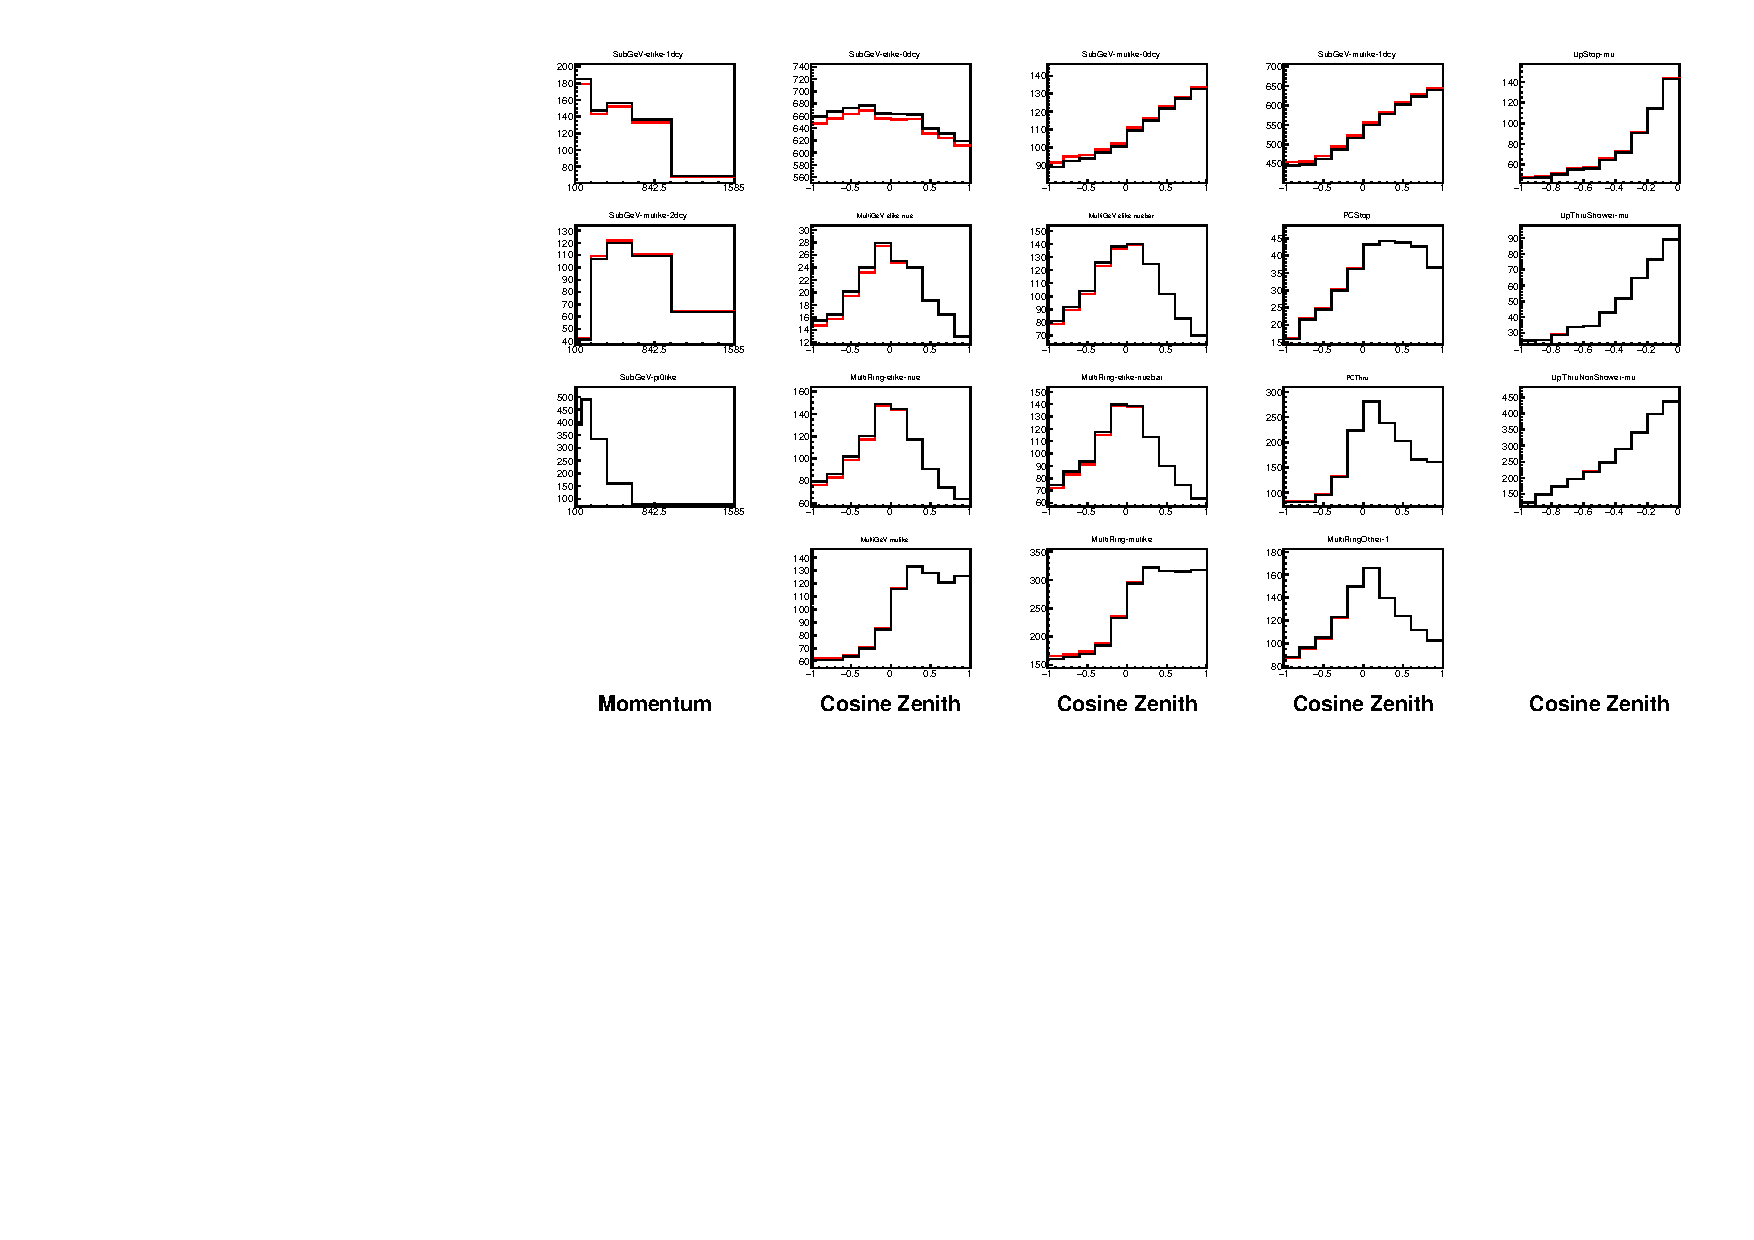
\includegraphics[width=\textwidth, trim={0mm 0mm 0mm 0mm}, clip,page=1]{Figures/Selections/HistogramComparison.pdf}
  \end{subfigure}
  \caption{Comparison of the SK-IV atmospheric samples between predictions made with the CP-violating Asimov A (Black) and CP-conserving Asimov B (Red) oscillation parameter sets (given in \autoref{tab:Theory_ParameterSets}). The subGeV samples CCRES and \quickmath{\pi^{0}}-like samples are given in their reconstructed lepton momentum. All other samples are presented in their reconstructed zenith angle projection.}
  \label{fig:SelsAndSysts_AllSampleComparison}
\end{sidewaysfigure}

\clearpage
\section{Near Detector Beam Samples}
\label{sec:SelsAndSysts_Sels_ND}

The near detector sample selections are documented in detail within \cite{t2k_tn_395} and summarised below. Samples are selected based upon which of the two Fine Grained Detector (FGD) the vertex is reconstructed in as well as the operating mode of the beam: FHC or RHC. Wrong-sign neutrino background samples are considered in the RHC mode in order to add additional constraints on model parameters. Samples from the wrong-sign component of the FHC beam mode are not included as they are statistically insignificant compared to those samples already listed.
%For additional constraints on model parameters, wrong-sign neutrino samples are also considered when the beam is operating in RHC mode.

The reconstruction algorithm uses a clustering algorithm to group hits within the TPC. It then adds information from the upstream FGD to form a track that passes through both sub-detectors. In FHC(RHC), the highest momentum negative(positive) curvature track is defined as the muon candidate. Before being assigned a sample, these candidate muon events must pass CC-inclusive cuts, as defined in \cite{t2k_tn_212}:

\begin{itemize}
\item Event Timing: The DAQ must be operational and the event must occur within the expected beam time window consistent with the beam spill
\item TPC Requirement: The muon-candidate track path must intercept one or more TPCs
\item Fiducial volume: The event must originate from within the fiducial volume defined in \cite{thesis_will}
\item Upstream Background: Remove events that have muon tracks that originate upstream of the FGDs by requiring no high-momentum tracks within \quickmath{150\text{mm}} upstream of the candidate vertex. Additionally, events that occur within the downstream FGD are vetoed if a secondary track starts within the upstream FGD
\item Broken track removal: All candidates where the muon candidate is broken in two are removed
\item Muon PID: Measurements of \quickmath{dE/dx} in a TPC are used to distinguish muon-like events, from electron-like or proton-like, using a likelihood cut
\end{itemize}

In addition to these cuts, RHC neutrino events also have to undergo the following cuts to aid in the separation of neutrino and antineutrino \cite{t2k_tn_246}:

\begin{itemize}
\item TPC Requirement: The track path must intercept TPC2
\item Positive Track: The highest momentum track must have a positive reconstructed charge
\item TPC1 Veto: Remove any events originating upstream of TPC1
\end{itemize}

Once all CC-inclusive events have been determined, they are further split by pion multiplicity: CC\quickmath{0\pi}, CC\quickmath{1\pi}, and CCOther. This breakdown targets the specific interaction modes CCQE, CCRES, and other CC background interactions, respectively. Pions in the TPCs and FGDs are selected by requiring a second track to be observed, which is separate from the muon track and is in the same beam spill window and sub-detector. If the pion originated within a FGD, it must also pass through the sequential downstream TPC (TPC2 for FGD1, TPC3 for FGD2). 

CC\quickmath{0\pi}, CC\quickmath{1\pi}, and CCOther samples are defined with the following cuts:

\finish{Understand pion cuts at ND}

\begin{itemize}
\item \textbf{\quickmath{\nu_{\mu} \text{CC} 0\pi} Selection}: No electrons in TPC and no charged pions or decay electrons within the TPC or FGD
\item \textbf{\quickmath{\nu_{\mu} \text{CC} 1\pi} Selection}: Exactly one charged pion in either the TPC or FGD, where the number of charged pions in the FGD is equal to the number of decay electrons
\item \textbf{\quickmath{\nu_{\mu} \text{CCOther}} Selection}: All events which are not classified into the above two selections
\end{itemize}

Counting the three selections for each FGD in FHC and RHC running, including the wrong-sign background in RHC, 18 near detector samples are used within this analysis. These samples are binned in reconstructed lepton momentum (illustrated in \autoref{fig:SelsAndSysts_Beam_NDPred}) and direction with respect to the beam. The binning is chosen such that each event has at least \quickmath{20} Monte Carlo events in each bin \cite{thesis_will}. This is to ensure that the bins are coarse enough to ensure the reduction of statistical errors, whilst also being fine enough to sample the high-resolution peak regions. The exact binning is detailed in \cite{thesis_will}.

\begin{figure}[h]
  \begin{subfigure}[t]{0.49\textwidth}
    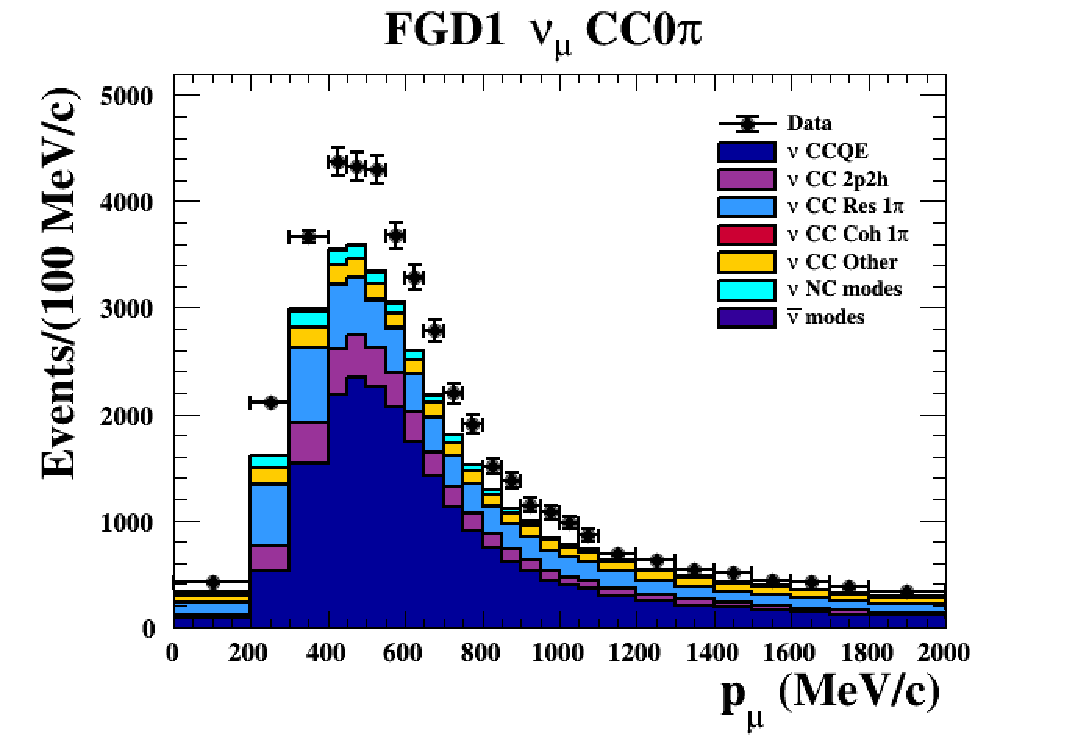
\includegraphics[width=\textwidth, trim={0mm 0mm 0mm 0mm}, clip,page=1]{Figures/Selections/Pmu_1D_modes_FGD1_numuCC_0pi_Data_prefit.pdf}
    %\subcaption{FGD1 FHC \quickmath{\nu_{\mu} 0\pi}}
  \end{subfigure}%
  \begin{subfigure}[t]{0.49\textwidth}
    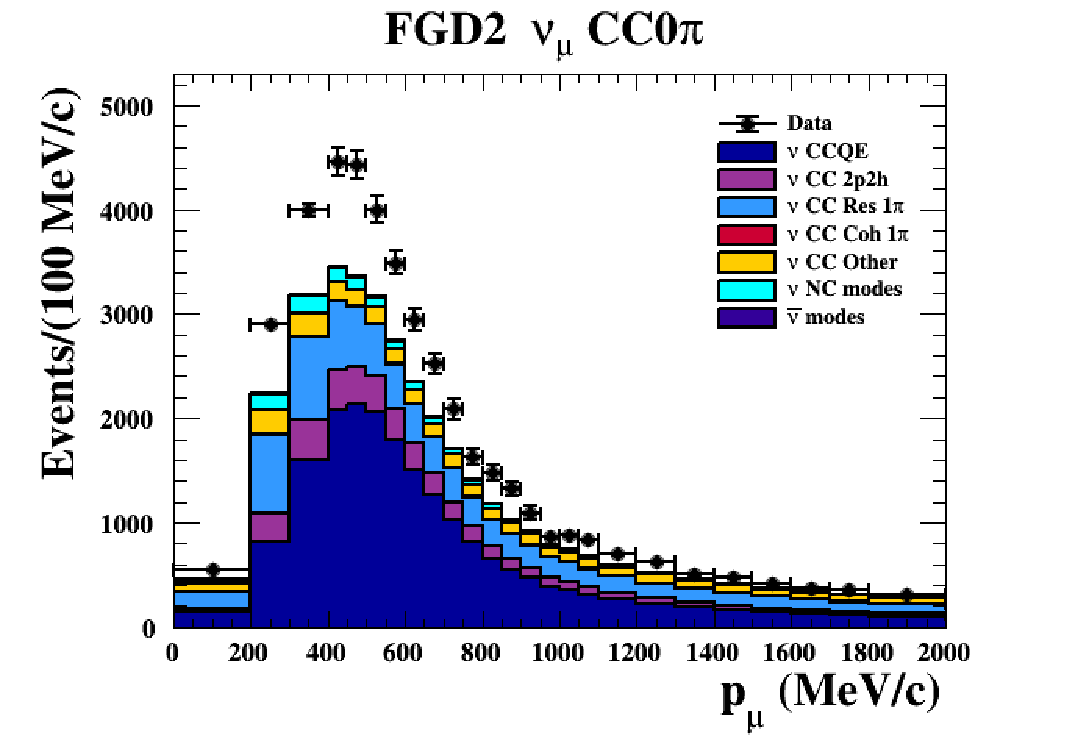
\includegraphics[width=\textwidth, trim={0mm 0mm 0mm 0mm}, clip,page=1]{Figures/Selections/Pmu_1D_modes_FGD2_numuCC_0pi_Data_prefit.pdf}
    %\subcaption{FGD2 FHC \quickmath{\nu_{\mu} 0\pi}}
  \end{subfigure}
  \begin{subfigure}[t]{0.49\textwidth}
    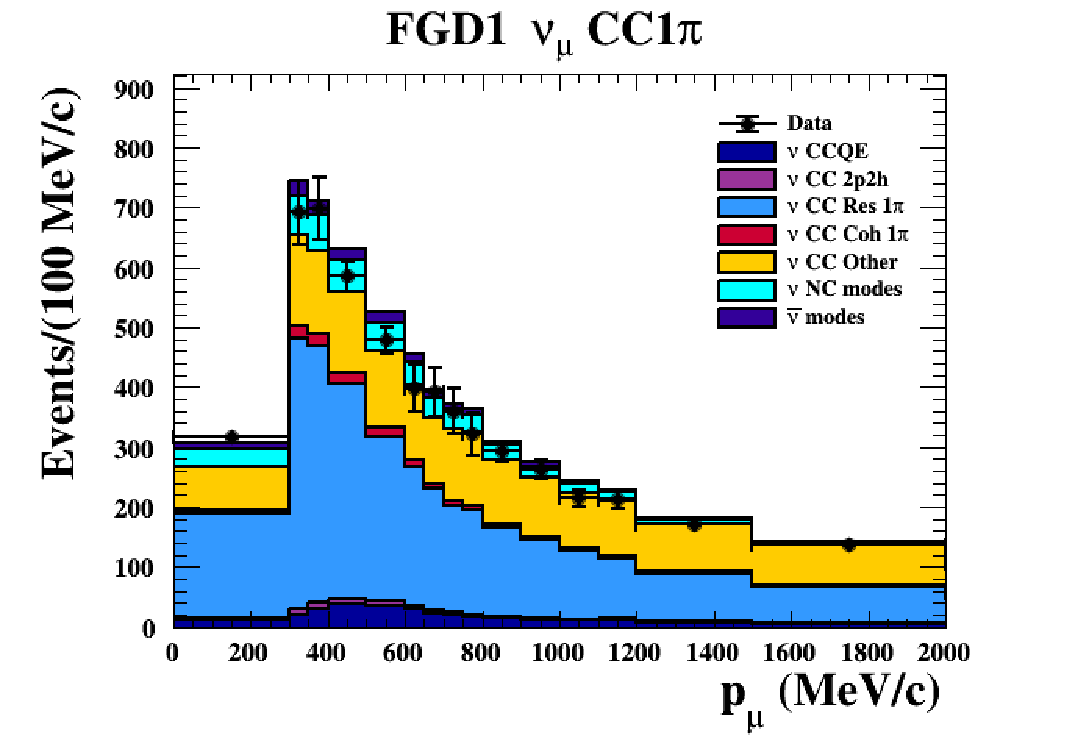
\includegraphics[width=\textwidth, trim={0mm 0mm 0mm 0mm}, clip,page=1]{Figures/Selections/Pmu_1D_modes_FGD1_numuCC_1pi_Data_prefit.pdf}
    %\subcaption{FGD1 FHC \quickmath{\nu_{\mu} 1\pi}}
  \end{subfigure}%
  \begin{subfigure}[t]{0.49\textwidth}
    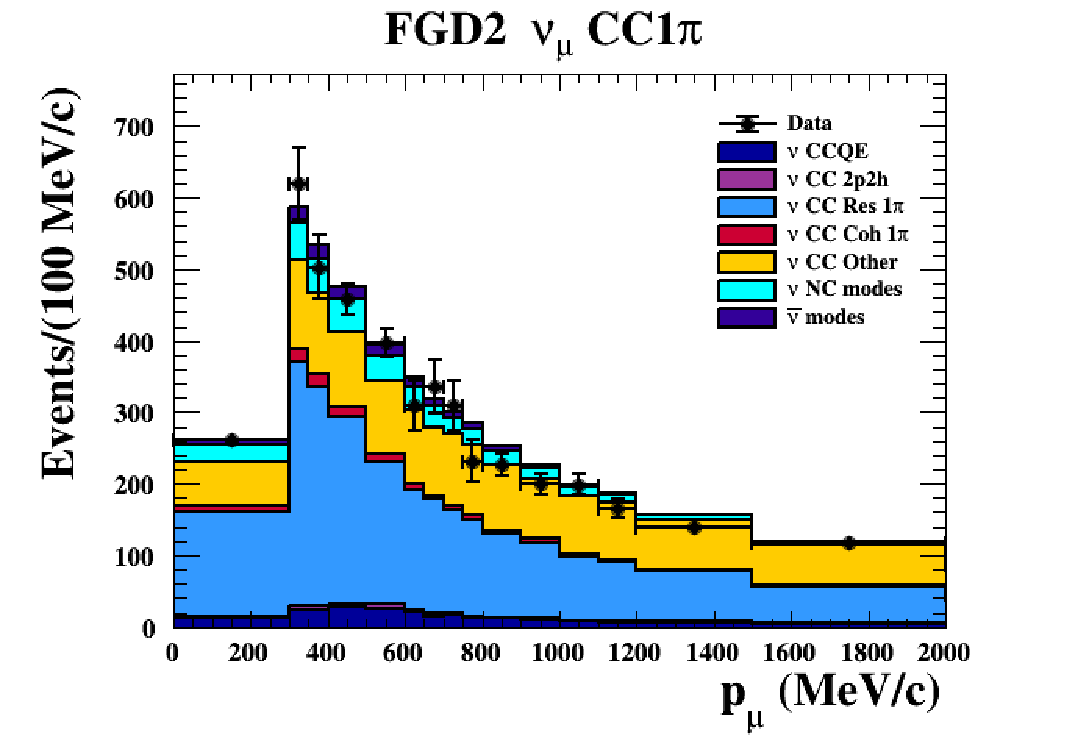
\includegraphics[width=\textwidth, trim={0mm 0mm 0mm 0mm}, clip,page=1]{Figures/Selections/Pmu_1D_modes_FGD2_numuCC_1pi_Data_prefit.pdf}
    %\subcaption{FGD2 FHC \quickmath{\nu_{\mu} 1\pi}}
  \end{subfigure}
  \begin{subfigure}[t]{0.49\textwidth}
    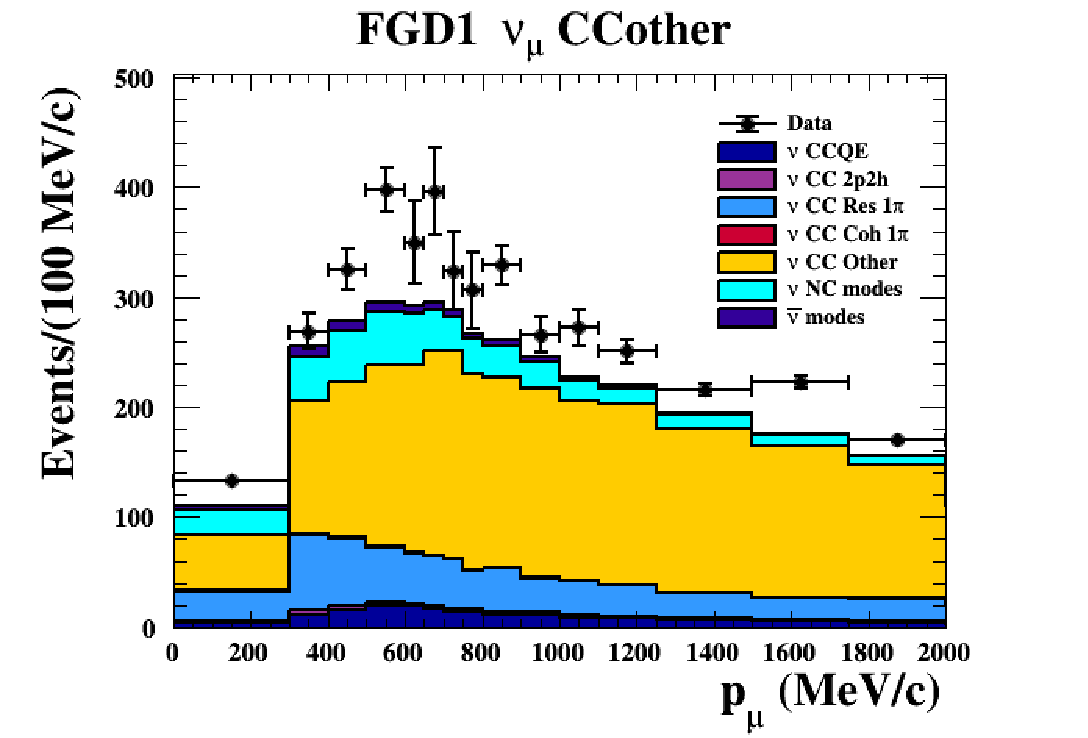
\includegraphics[width=\textwidth, trim={0mm 0mm 0mm 0mm}, clip,page=1]{Figures/Selections/Pmu_1D_modes_FGD1_numuCC_other_Data_prefit.pdf}
    %\subcaption{FGD1 FHC \quickmath{\nu_{\mu} \text{Other}}}
  \end{subfigure}%
  \begin{subfigure}[t]{0.49\textwidth}
    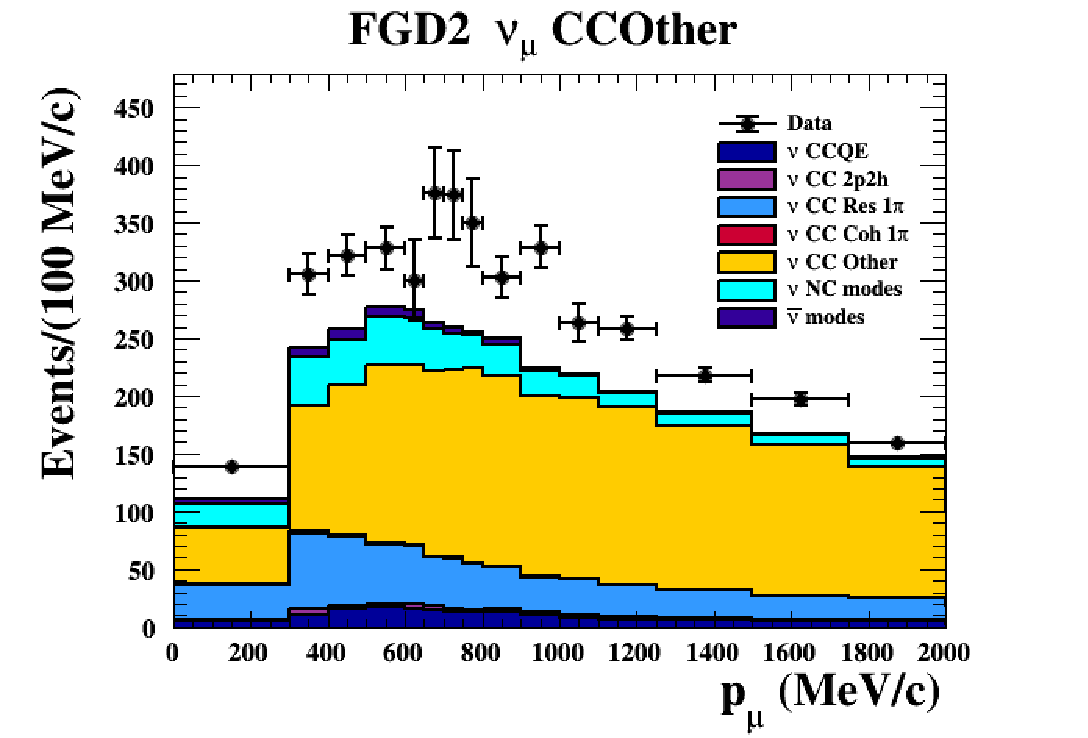
\includegraphics[width=\textwidth, trim={0mm 0mm 0mm 0mm}, clip,page=1]{Figures/Selections/Pmu_1D_modes_FGD2_numuCC_other_Data_prefit.pdf}
    %%\subcaption{FGD2 FHC \quickmath{\nu_{\mu} \text{Other}}}
  \end{subfigure}
  \caption{The nominal Monte Carlo predictions compared to data for the FGD1 and FGD2 samples in neutrino beam mode, broken down into the \quickmath{CC\nu_{\mu} 0\pi}, \quickmath{CC\nu_{\mu} 1\pi} and \quickmath{CC\nu_{\mu} \text{ Other}} categories. Figures taken from \cite{t2k_tn_395}.}
  \label{fig:SelsAndSysts_Beam_NDPred}
\end{figure}

\section{Far Detector Beam Samples}
\label{sec:SelsAndSysts_Sels_FD}

The beam neutrino events which occur at the SK detector, which pass the reduction cuts detailed in \autoref{sec:Simulations_Reduction}, are separated based on whether the beam was operating in FHC or RHC mode. The events are then separated into three samples: electron-like (\quickmath{1\text{R}e}), muon-like (\quickmath{1\text{R}\mu}), and CC\quickmath{1\pi^{+}}-like (\quickmath{1\text{R}e1de}) which are observed as electron-like events with an associated decay electron \cite{t2k_tn_399}. As discussed in \autoref{sec:SelsAndSysts_Sels_Atms}, positively charged pions emitted from neutrino interactions are more likely to produce decay electrons than negatively charged pions. Consequently, the CC\quickmath{1\pi^{+}}-like sample is only selected when the beam is operating in FHC mode. Therefore, five beam samples measured at SK are used in this analysis.
%As the T2K oscillation analysis has evolved over the years and the selections changed, the sample names are suffixed with \texttt{2020} to indicate they are the samples used within the 2020 T2K oscillation analysis.

The fiducial volume definition for beam samples is slightly different from that used for the atmospheric samples.  It uses both the distance to the closest wall (\texttt{dWall}) and the distance to the wall along the trajectory of the particle (\texttt{toWall}). This allows events that originate close to the wall but are facing into the tank to be included within the analysis, which would have otherwise been removed. These additional events are beneficial for a statistics-limited experiment. The exact cut values for both \texttt{dWall} and \texttt{toWall} are different for each of the three types of sample and are optimised based on T2K sensitivity to \quickmath{\delta_{CP}} \cite{t2k_tn_318, t2k_tn_319}. They are:

\paragraph{\quickmath{1\text{R}e} event selection}

For an event to be classified as a \quickmath{1\text{R}e}-like, the event must satisfy:

\begin{itemize}
\item Fully-contained and have \texttt{dWall} \quickmath{>80\text{cm}} and \texttt{toWall} \quickmath{>170\text{cm}}
\item Total of one ring which is reconstructed as electron-like with reconstructed momentum \quickmath{P_{e} > 100\text{MeV}}
\item Zero decay electrons are associated with the event
\item Passes \quickmath{\pi^{0}} rejection cut discussed in \autoref{sec:Simulation_Reconstruction}
\end{itemize}

The zero decay electron	cut removes non-CCQE interactions and the \quickmath{\pi^{0}} rejection cut is designed to remove neutral current \quickmath{\pi^{0}} background events which can be easily reconstructed as \quickmath{1\quickmath{R}e}-like events.

The zero decay electron cut removes non-CCQE interactions and the \quickmath{\pi^{0}} rejection cut is designed to remove neutral current \quickmath{\pi^{0}} background events which can be easily reconstructed as \quickmath{1\quickmath{R}e}-like events.                 

\paragraph{CC\quickmath{1\pi^{+}} event selection} This event selection is very similar to that of the \quickmath{1\text{R}e} sample. The only differences are that the \texttt{dWall} and \texttt{toWall} criteria are changed to \quickmath{>50\text{cm}} and \quickmath{>270\text{cm}}, respectively, and exactly one decay electron is required from the \quickmath{\pi^{+}} decay. 

\paragraph{\quickmath{1\text{R}\mu} event selection}

A \quickmath{1\text{R}\mu}-like event is determined by the following cuts:

\begin{itemize}
\item Fully-contained and have \texttt{dWall} \quickmath{>50\text{cm}} and \texttt{toWall} \quickmath{>250\text{cm}}
\item Total of one ring which is reconstructed as muon-like with reconstructed momentum \quickmath{P_{\mu} > 200\text{MeV}}
\item Fewer than two decay electrons are associated with the event
\item Passes \quickmath{\pi^{+}} rejection cut discussed in \autoref{sec:Simulation_Reconstruction}
\end{itemize}

%As pions and muons have similar masses, the Cherenkov rings they generate have similar opening angles. To enhance the purity, the events have to pass the \quickmath{\pi^{+}} rejection cut which is specifically optimised to separate the two types of events.

All of these samples are binned in reconstructed neutrino energy. This is possible under a particular interaction mode assumption, as the direction from the source is known extremely well. For the \quickmath{1\text{R}e}-like and \quickmath{1\text{R}\mu}-like samples,

\begin{equation}
  \label{sec:SelsAndSysts_Erec_CCQE}
  E^{rec}_{\nu} = \frac{(M_{N}-V_{nuc})E_{l} - m_{l}^{2}/2 + M_{N}V_{nuc} - V_{nuc}^{2}/2 + (M_{P}^{2} + M_{N}^{2})/2}{M_{N} - V_{nuc} - E_{l} + P_{l}\cos(\theta_{beam})}.
\end{equation}

Where \quickmath{M_{N}}, \quickmath{M_{P}} and \quickmath{m_{l}} are the masses of the neutron, proton and outgoing lepton, respectively. \quickmath{V_{nuc} = 27\text{MeV}} is the binding energy of the oxygen nucleus \cite{t2k_tn_399}, \quickmath{\theta_{beam}} is the angle between the beam and the direction of the outgoing lepton, and \quickmath{E_{l}} and \quickmath{P_{l}} are the energy and momentum of that outgoing lepton.

\begin{figure}[h]
  \begin{subfigure}[t]{0.49\textwidth}
    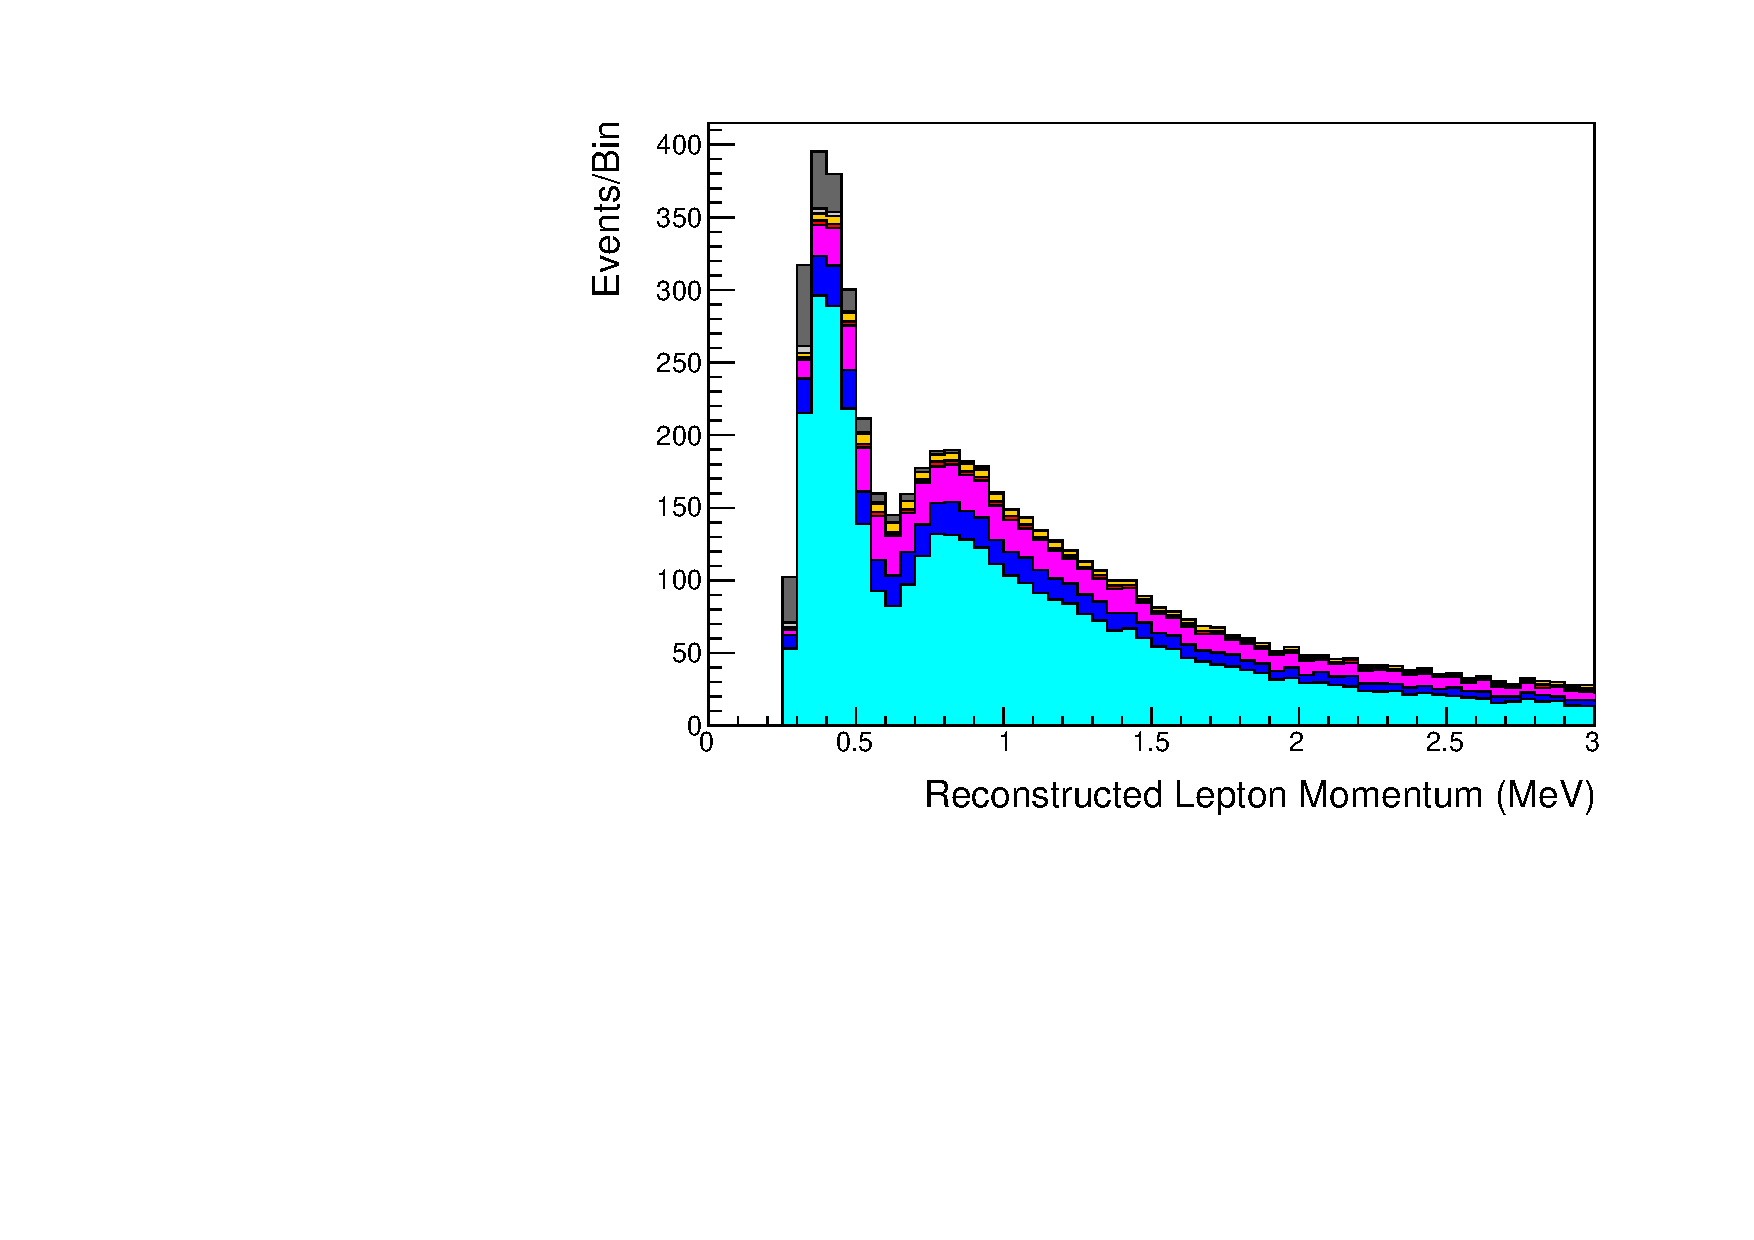
\includegraphics[width=\textwidth, trim={0mm 0mm 0mm 0mm}, clip,page=1]{Figures/Selections/FHC1Rmu-2020_X.pdf}
    \subcaption{FHC \quickmath{1\text{R}\mu}}
  \end{subfigure}%
  \begin{subfigure}[t]{0.49\textwidth}
    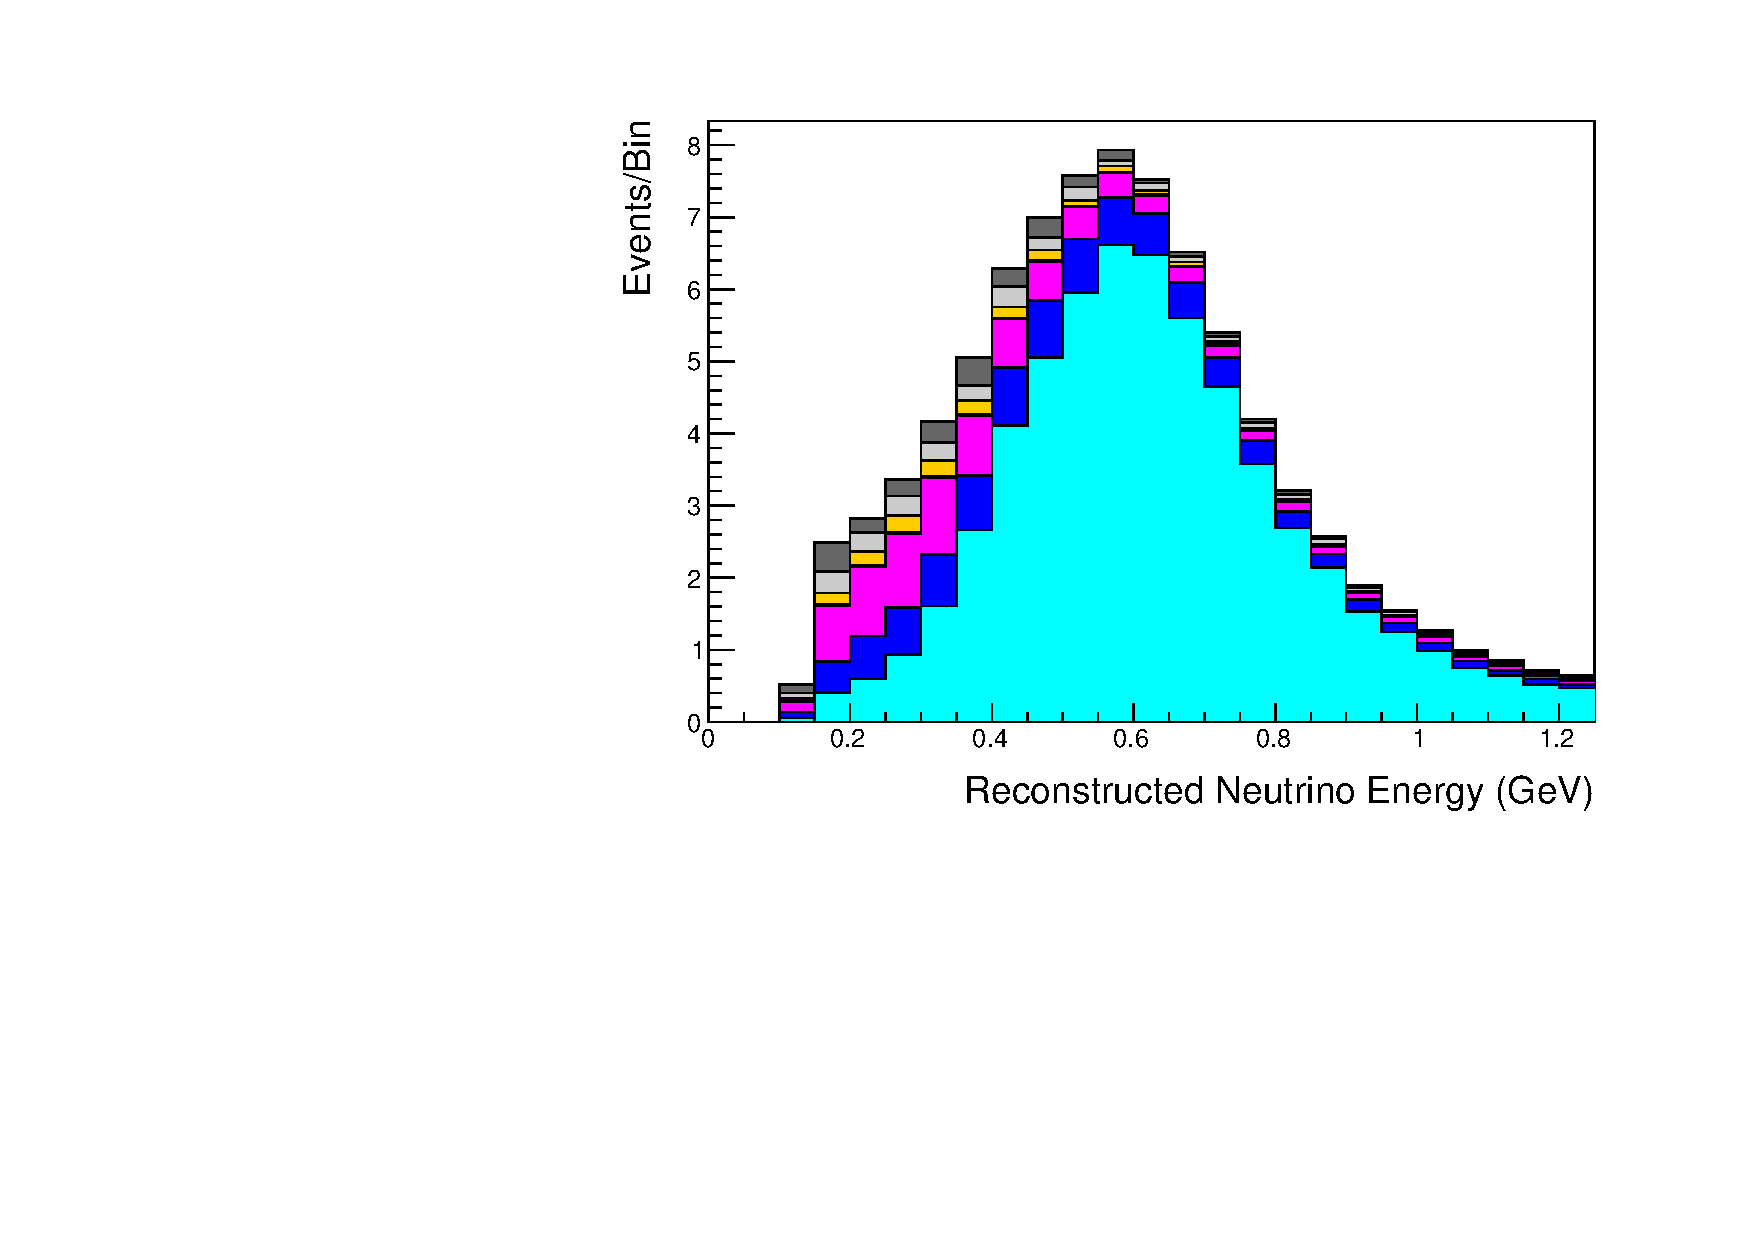
\includegraphics[width=\textwidth, trim={0mm 0mm 0mm 0mm}, clip,page=1]{Figures/Selections/FHC1Re-2020_X.pdf}
    \subcaption{FHC \quickmath{1\text{R}e}}
  \end{subfigure}
  \begin{subfigure}[t]{0.49\textwidth}
    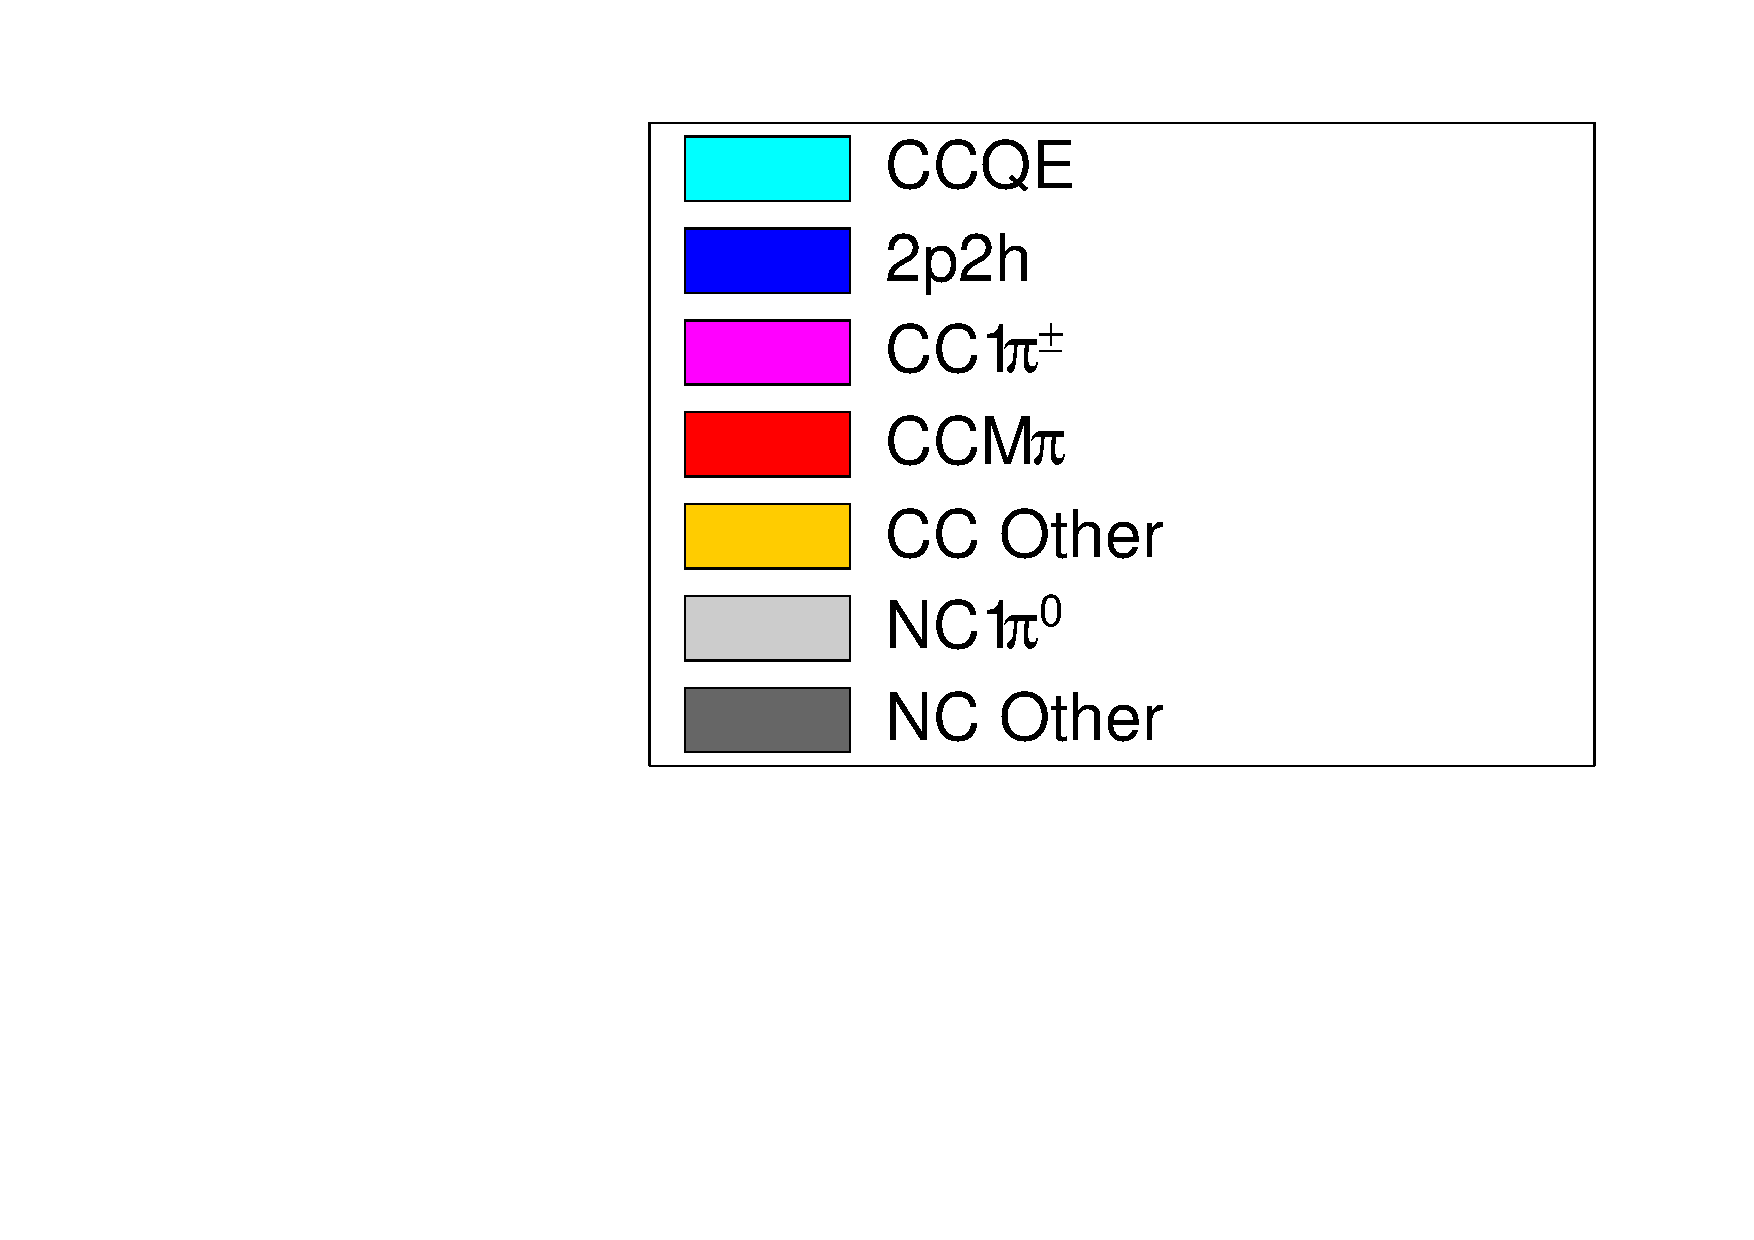
\includegraphics[width=\textwidth, trim={0mm 0mm 0mm 0mm}, clip,page=1]{Figures/Selections/Legend.pdf}
  \end{subfigure}%
  \begin{subfigure}[t]{0.49\textwidth}
    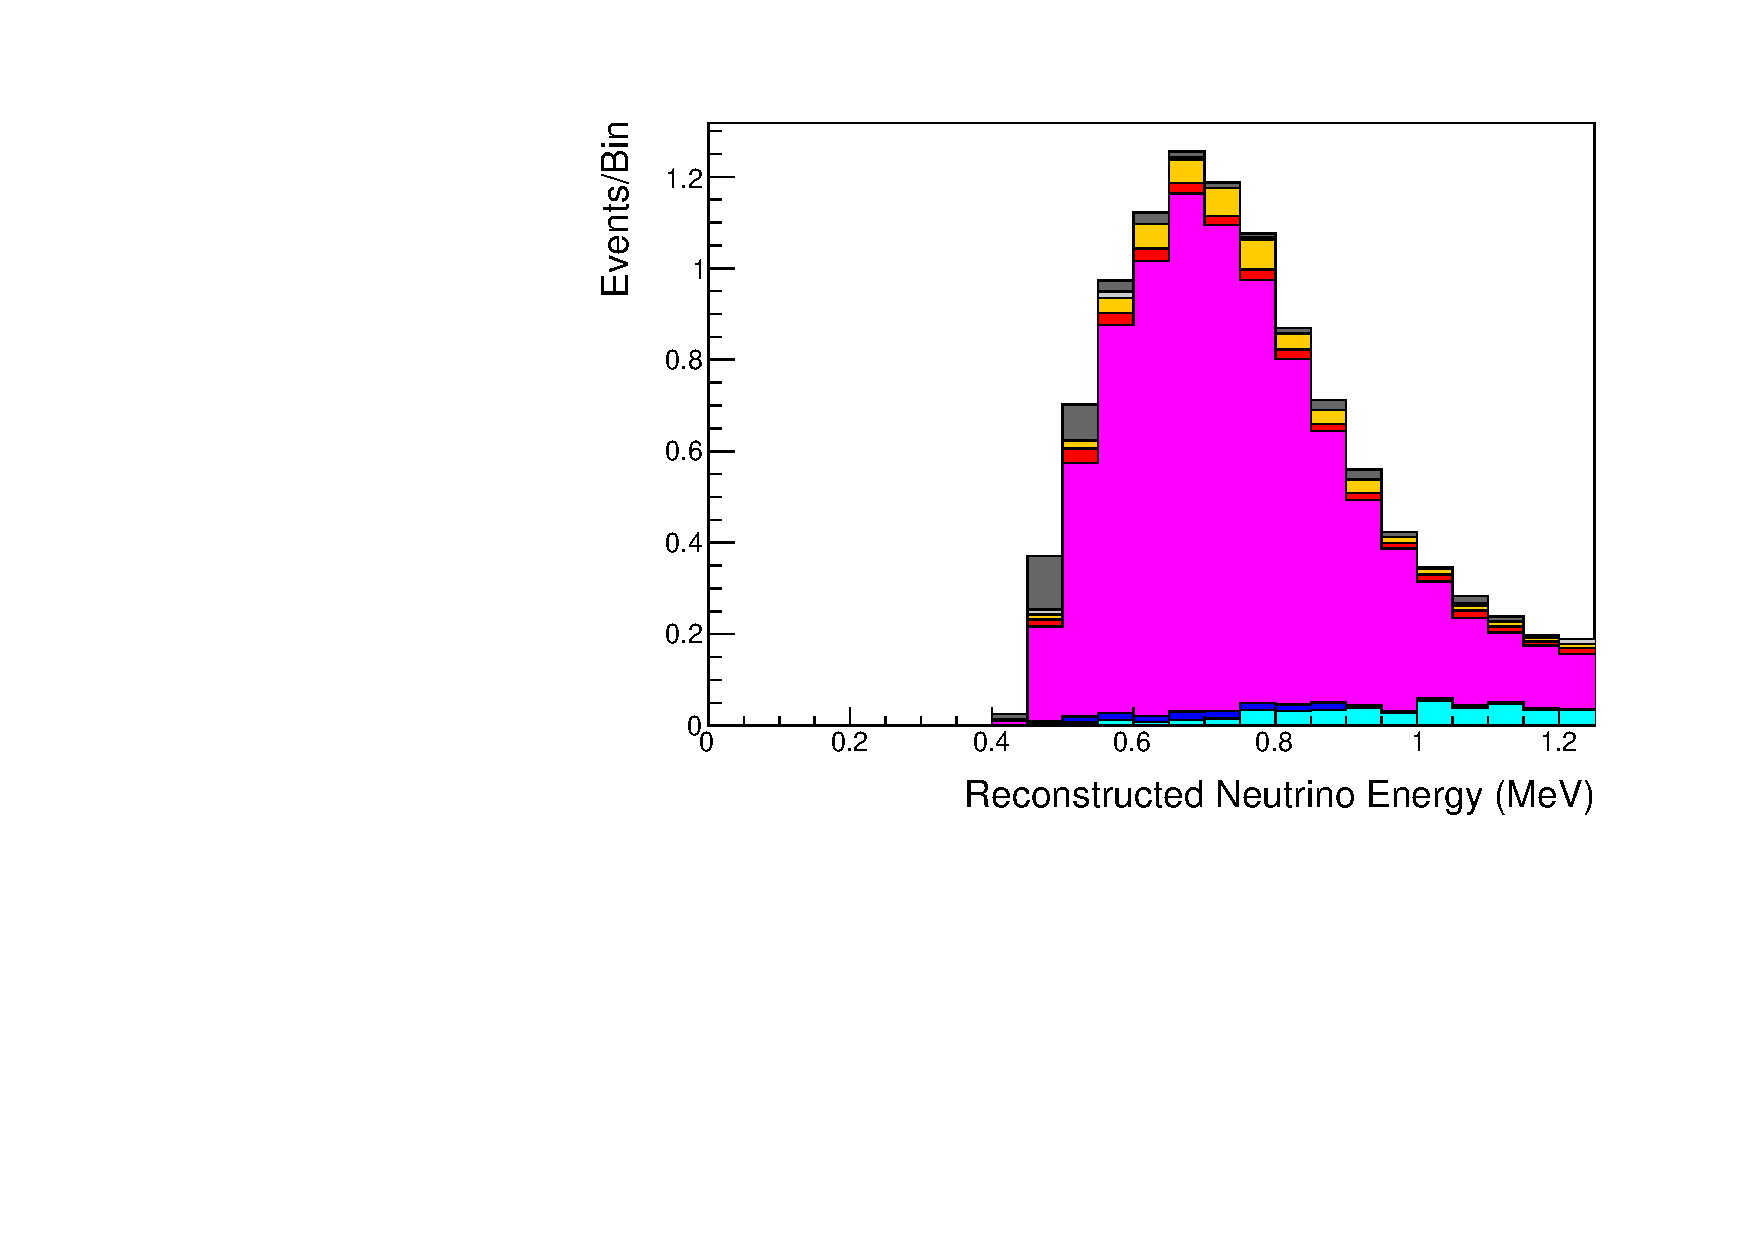
\includegraphics[width=\textwidth, trim={0mm 0mm 0mm 0mm}, clip,page=1]{Figures/Selections/FHCCC1pi-2020_X.pdf}
    \subcaption{FHC CC\quickmath{1\pi^{+}}}
  \end{subfigure}
  \caption{The reconstructed neutrino energy, as defined by \autoref{sec:SelsAndSysts_Erec_CCQE} and \autoref{sec:SelsAndSysts_Erec_CCRES}, for the \quickmath{1\text{R}\mu}-like, \quickmath{1\text{R}e}-like, and CC\quickmath{1\pi^{+}}-like samples. The AsimovA oscillation parameters are assumed (given in \autoref{tab:Theory_ParameterSets}). These samples are the FHC mode samples. For ease of viewing, the \quickmath{1\text{R}\mu} sample only shows the \quickmath{0. \leq E^{rec}_{\nu} < 3.0 \text{GeV}} but the binning extends to \quickmath{30.0 \text{GeV}}.}
  \label{fig:SelsAndSysts_Beam_ERecSpectra}
\end{figure}

The reconstructed neutrino energy of the CC\quickmath{1\pi^{+}}-like events also accounts for the delta resonance produced within the interaction,

\begin{equation}
  \label{sec:SelsAndSysts_Erec_CCRES}
  E^{rec}_{\nu} = \frac{2M_{N}E_{l} + M_{\Delta^{++}}^{2} - M_{N}^{2} - m_{l}^{2}}{2(M_{N} - E_{l} + P_{l}\cos(\theta_{beam}))}.
\end{equation}

Where \quickmath{M_{\Delta^{++}}} is the mass of the delta baryon. Binding energy effects are not considered as a two-body process, with the delta baryon, is assumed. This follows the T2K oscillation analysis presented in \cite{Dunne2020-uf}, although recent developments of the interaction model in the latest T2K oscillation analysis do include effects from binding energy in this calculation \cite{t2k_tn_414}.

The reconstructed neutrino energy for the FHC samples is illustrated in \autoref{fig:SelsAndSysts_Beam_ERecSpectra}. As expected, the \quickmath{1\text{R}\mu}-like and \quickmath{1\text{R}e}-like samples are heavily dominated by CCQE interactions, with smaller contributions from 2p2h meson exchange and resonant pion production interactions. The CC\quickmath{1\pi^{+}}-like sample predominantly consists of charged current resonant pion production interactions. The \quickmath{1\text{R}e}-like and CC\quickmath{1\pi^{+}}-like samples are also binned by the angle between the neutrino beam and the reconstructed lepton momentum. This is to aid in charged current and neutral current separation, as indicated in \autoref{fig:SelsAndSysts_Beam_FHC1ReThetaSpectra}. This is because the neutral current backgrounds are predominantly due to \quickmath{\pi^{0}}-decays, which decay into two \quickmath{\gamma} rays. The opening angle of which (alongside the different final state kinematics) can produce a slightly broader angular distribution compared to the final state particles originating from charged current \quickmath{\nu_{e}} interactions.

\begin{figure}[h]
  \begin{subfigure}[t]{\textwidth}
    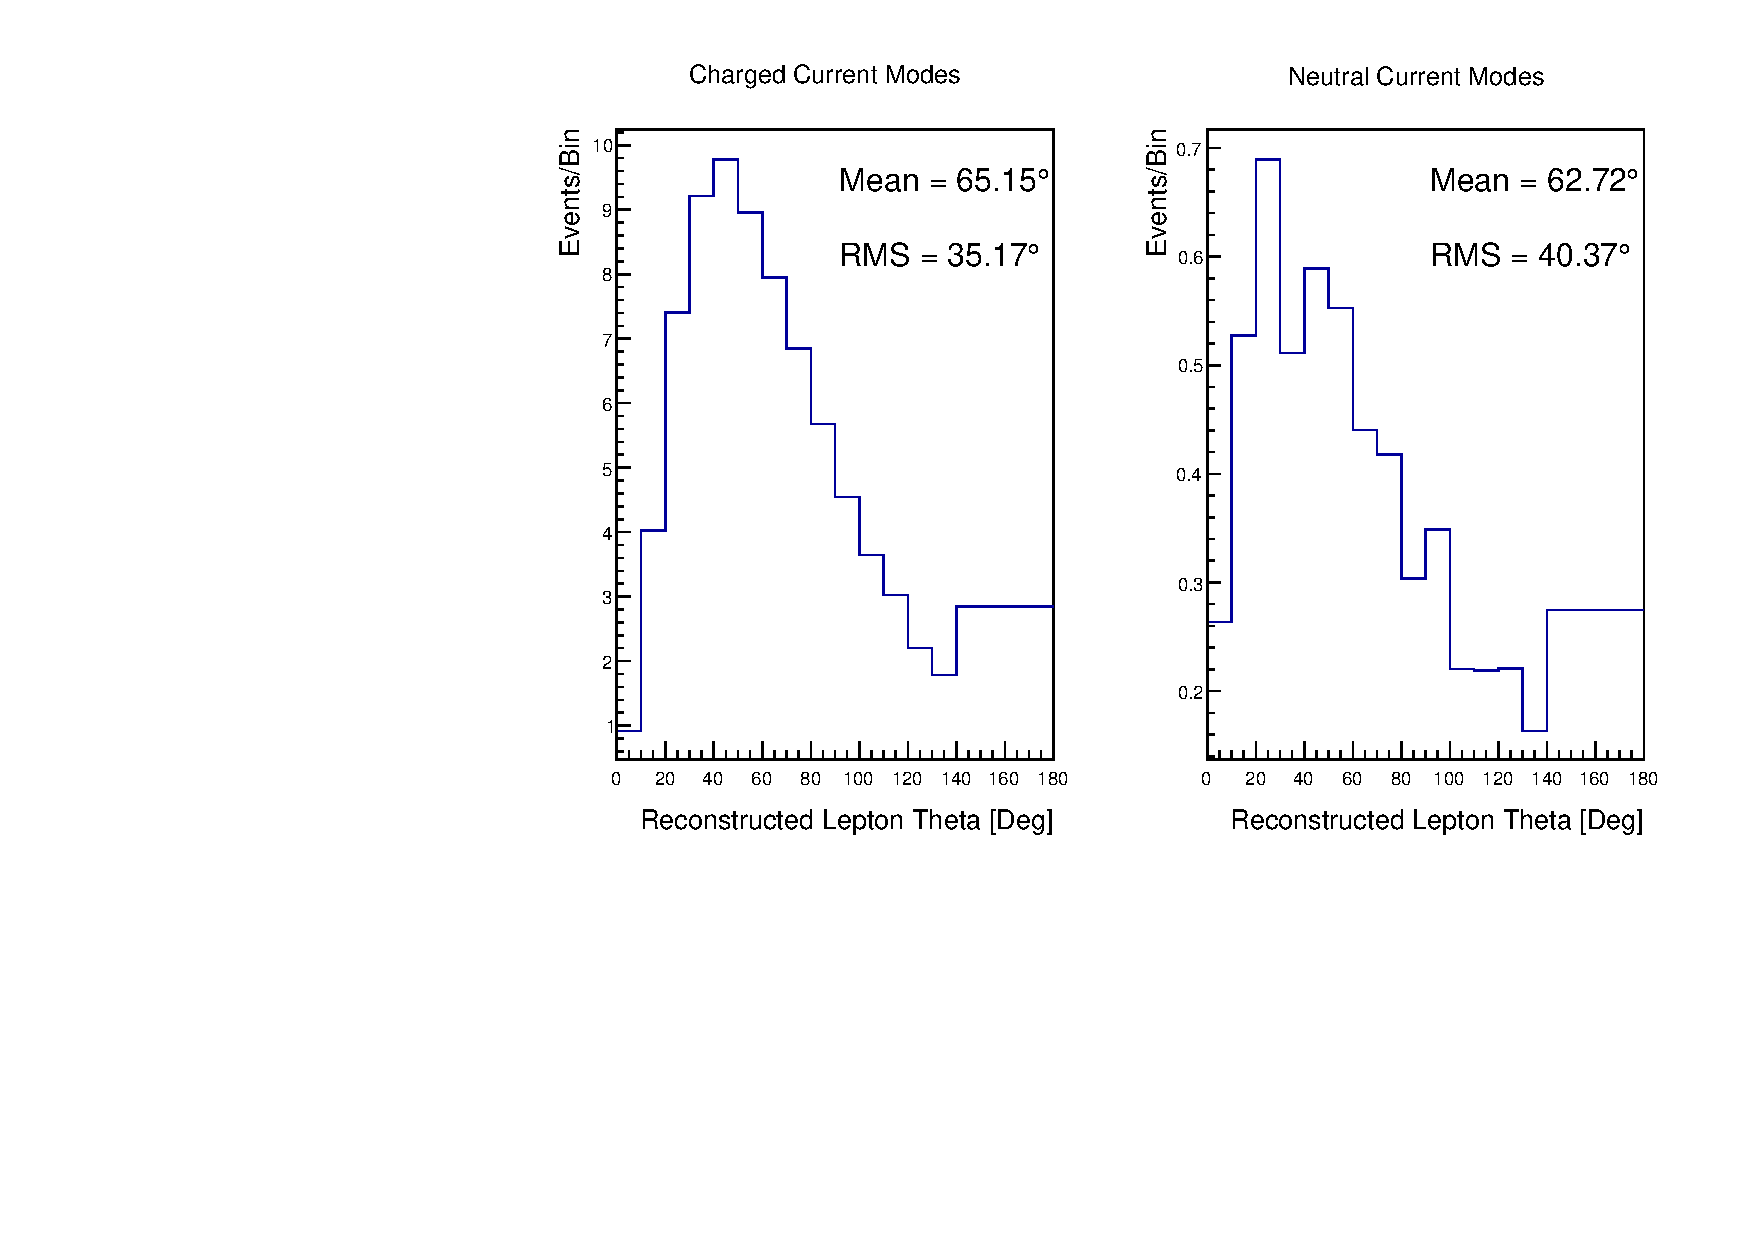
\includegraphics[width=\textwidth, trim={0mm 0mm 0mm 0mm}, clip,page=1]{Figures/Selections/1DSpectra_FHC1Re-2020.pdf}
  \end{subfigure}
  \caption{The distribution of the angle between the neutrino beam direction and the reconstructed final state lepton, for the FHC \quickmath{1\text{R}e}-like sample. The distribution is broken down by neutrino interaction mode into charged current (left) and neutral current (right) components. Asimov A oscillation parameter sets are assumed (given in \autoref{tab:Theory_ParameterSets}). The RMS of the charged and neutral current plots are \quickmath{35.17\degree} and \quickmath{40.37\degree}, respectively.}
  \label{fig:SelsAndSysts_Beam_FHC1ReThetaSpectra}
\end{figure}

\clearpage
\section{Systematic Uncertainties}
\label{sec:SelsAndSysts_Systs}

The systematic model parameters for this analysis are split into groups, or blocks, depending on their purpose. They consist of flux uncertainties, neutrino-matter interaction systematics, and detector efficiencies. There are also uncertainties on the oscillation parameters to which this analysis is not sensitive, namely \quickmath{\Delta m^{2}_{21}} and \quickmath{\sin^{2}(\theta_{12})}. These oscillation parameter uncertainties are taken from the 2020 PDG measurements \cite{Particle_Data_Group2020-ms}. As described in \autoref{chap:MarkovChainMonteCarlo}, each model parameter used within this analysis requires a prior uncertainty. This is provided via separate covariance matrices for each block. The covariance matrices can include prior correlations between parameters within a single block, but the separate treatment means prior correlations can not be included for parameters in different groups. Some parameters in these models have no reasonably motivated uncertainties and are assigned flat priors which do not modify the likelihood penalty. In practice, these flat prior parameters are actually assigned a Gaussian with a very large width to ensure the covariance matrix is positive definite. They are then checked at run time to determine if they contribute to the likelihood. The flux, neutrino interaction, and detector modeling simulations have already been discussed in \autoref{sec:Simulations_Simulation} and \autoref{sec:Simulation_Reconstruction}. The uncertainties invoked within each of these models are described below.

\subsection{Beam Flux}
\label{sec:SelsAndSysts_Systs_BeamFlux}

The neutrino beam flux systematics are based upon the uncertainty in the modeling of the components of the beam simulation. This includes the model of hadron productions and reinteractions, the shape, intensity, and alignment of the beam with respect to the target, and the uniformity of the magnetic field produced by the horn, alongside other effects. The uncertainty, as a function of neutrino energy, is illustrated in \autoref{fig:SelsAndSysts_BeamFluxSysts} which includes a depiction of the total uncertainty as well as the contribution from individual components. The uncertainty around the peak of the energy distribution (\quickmath{E_{\nu} \sim 0.6\text{GeV}}) is dominated by uncertainties in the beam profile and alignment. Outside of this region, uncertainties on hadron production dominate the error.

\begin{figure}[h]
  \begin{subfigure}[t]{\textwidth}
    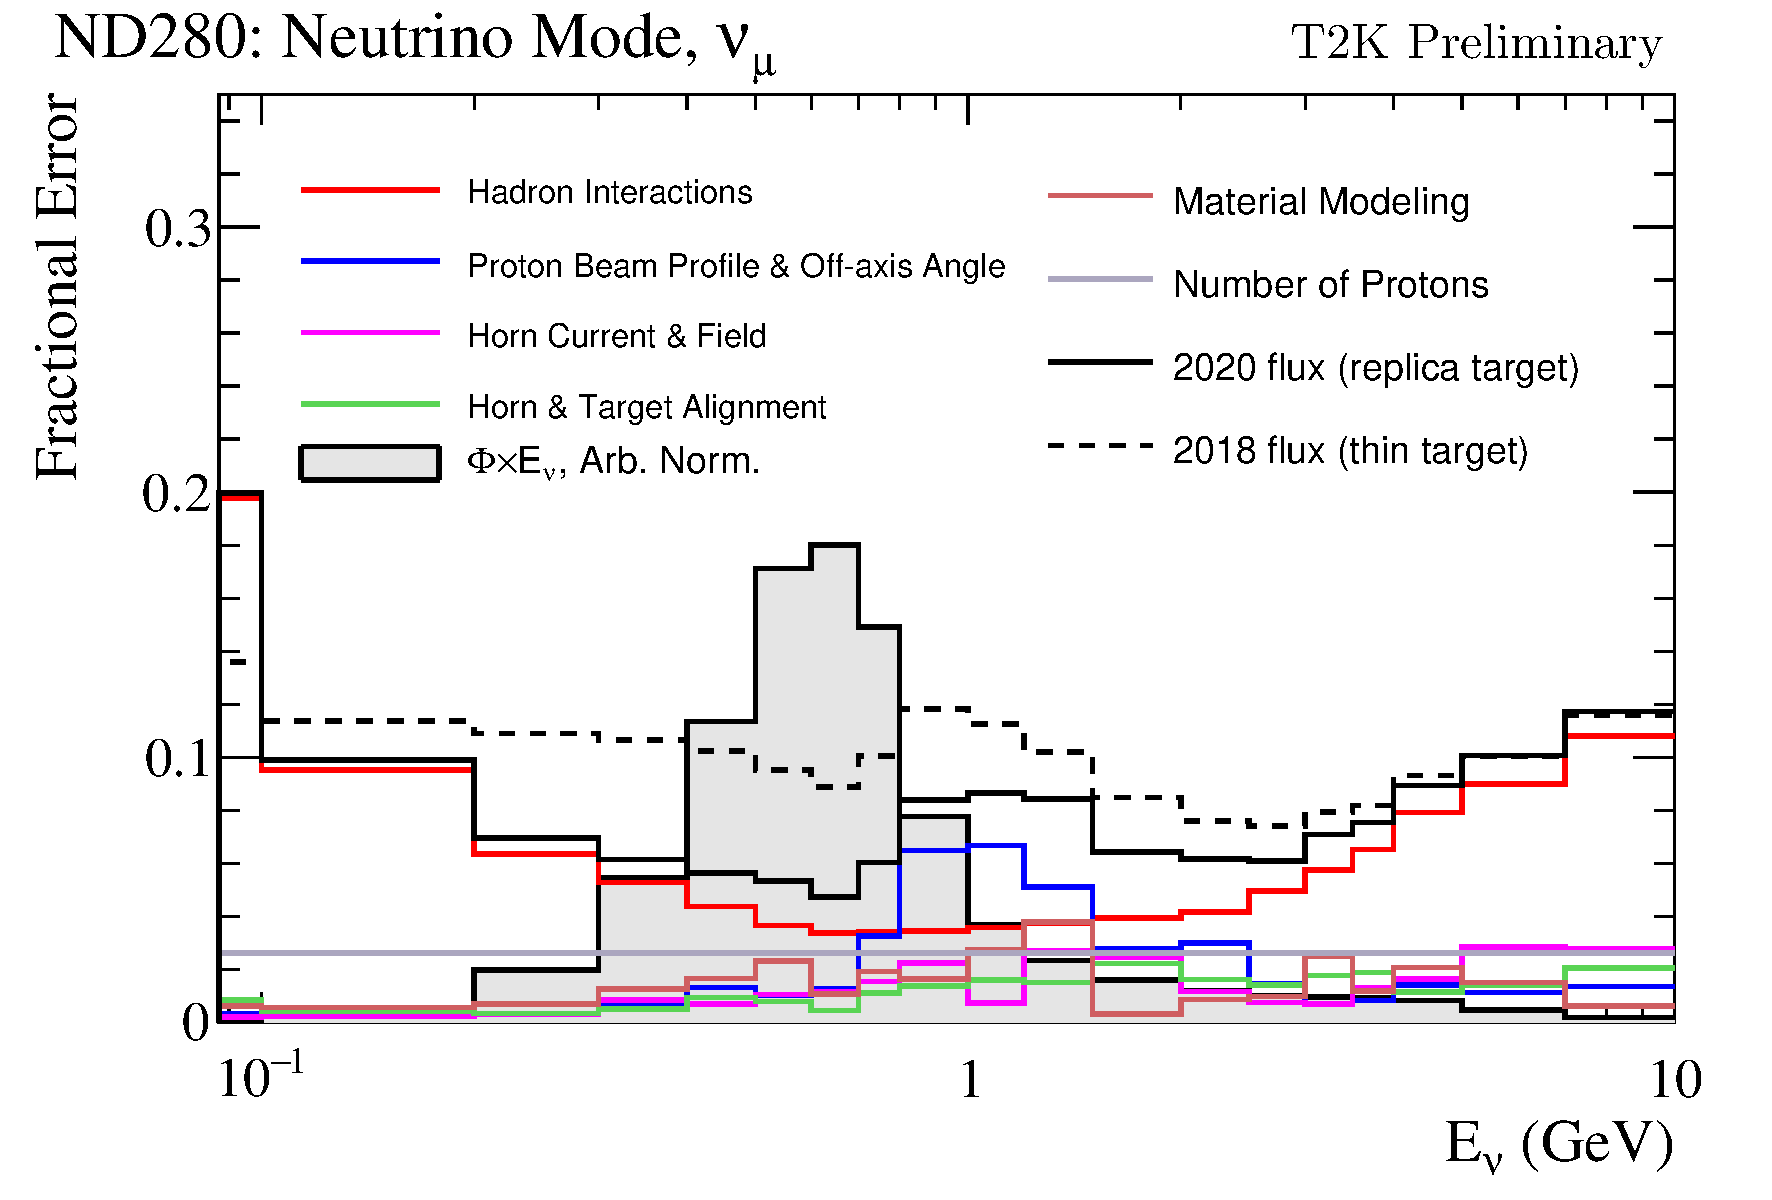
\includegraphics[width=\textwidth, trim={0mm 0mm 0mm 0mm}, clip,page=1]{Figures/Selections/flux_uncertainty_covariance_plots_addcorrnd_compwv3_flux_error_t2k_nd5_fhc_numu.pdf}
  \end{subfigure}
  %\begin{subfigure}[t]{\textwidth}
  %  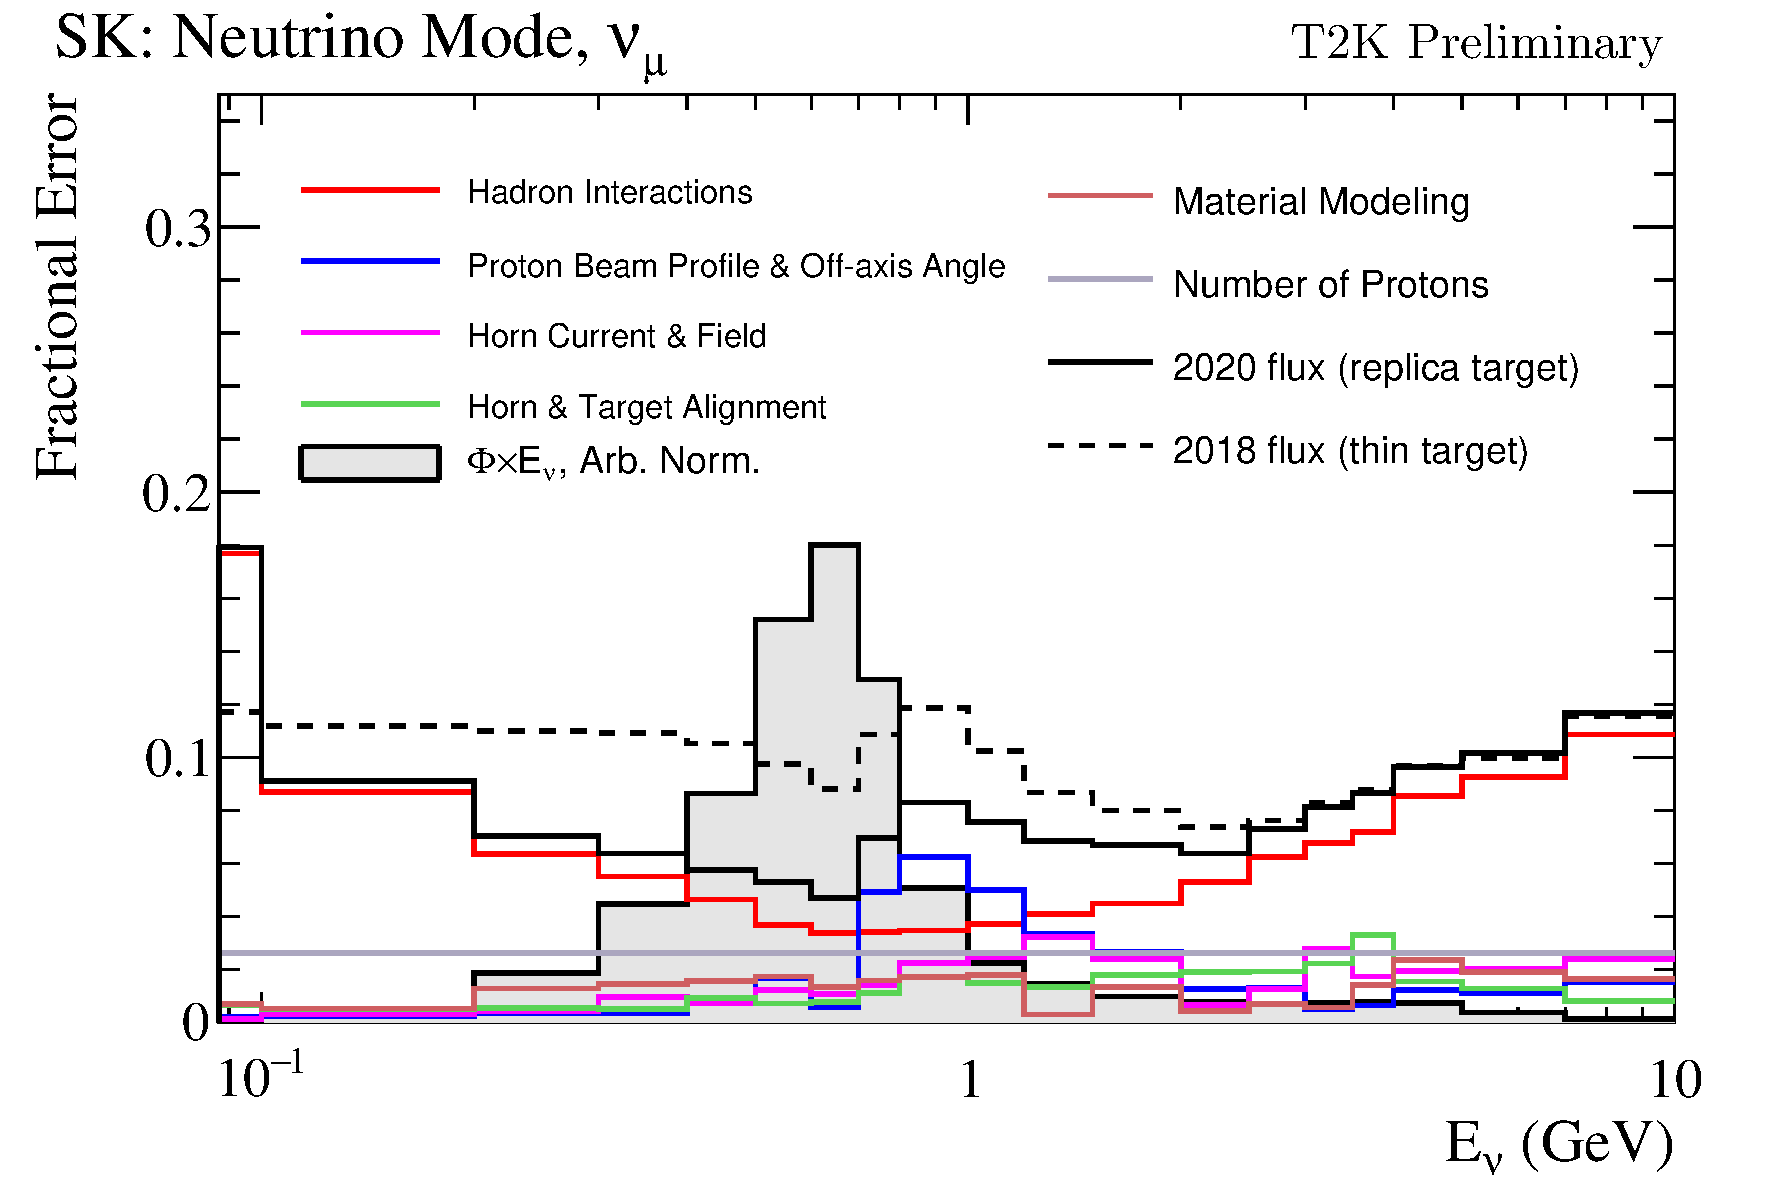
\includegraphics[width=\textwidth, trim={0mm 0mm 0mm 0mm}, clip,page=1]{Figures/Selections/flux_uncertainty_covariance_plots_addcorrnd_compwv3_flux_error_t2k_sk_fhc_numu.pdf}
  %\end{subfigure}
  \caption{The total uncertainty evaluated on the near detector \quickmath{\nu_{\mu}} flux prediction constrained by the replica-target data, illustrated as a function of neutrino energy. The solid(dashed) line indicates the uncertainty used within this analysis(the T2K 2018 analysis \cite{t2k_neutrino2018}). The solid histogram indicates the neutrino flux as a function of energy. Figure taken from \cite{t2k_tn_354}.}
  \label{fig:SelsAndSysts_BeamFluxSysts}
\end{figure}

The beam flux uncertainties are described by one hundred parameters. They are split between the ND280 and SK detectors and binned by neutrino flavour: \quickmath{\nu_{\mu}}, \quickmath{\bar{\nu}_{\mu}}, \quickmath{\nu_{e}} and \quickmath{\bar{\nu}_{e}}. The response is then broken down as a function of neutrino energy. The bin density in the neutrino energy is the same for the \quickmath{\nu_{\mu}} in FHC and \quickmath{\bar{\nu}_{\mu}} in RHC beams, and narrows for neutrino energies close to the oscillation maximum of \quickmath{E_{\nu} = 0.6\text{GeV}}. This binning is specified in \autoref{tab:SelsAndSysts_BeamFluxBinEdges}. All of these systematic uncertainties are applied as normalisation parameters with Gaussian priors centered at \quickmath{1.0} and error specified from a covariance matrix provided by the T2K beam group \cite{t2k_tn_354}.

\begin{table}[ht!]
    \centering
    \begin{tabular}{c|c|c}
      \hline
      Neutrino Flavour & Sign & Neutrino Energy Bin Edges (GeV) \\
      \hline
      \quickmath{\mu} & Right & \quickmath{0.,0.4,0.5,0.6,0.7,1.,1.5,2.5,3.5,5.,7.,30.} \\
      \quickmath{\mu} & Wrong & \quickmath{0.,0.7,1.,1.5,2.5,30.} \\
      \quickmath{e} & Right & \quickmath{0.,0.5,0.7,0.8,1.5,2.5,4.,30.} \\
      \quickmath{e} & Wrong & \quickmath{0.,2.5,30.} \\
      \hline
      \hline
    \end{tabular}
    \caption{The neutrino energy binning for the different neutrino flavours. ``Right'' sign indicates neutrinos in the FHC beam and antineutrinos in the RHC beam. ``Wrong'' sign indicates antineutrinos in the FHC beam and neutrinos in the RHC beam. The binning of the detector response is identical for the FHC and RHC modes as well as at ND280 and SK.}
    \label{tab:SelsAndSysts_BeamFluxBinEdges}
\end{table}

\subsection{Atmospheric Flux}
\label{sec:SelsAndSysts_Systs_AtmFlux}
The atmospheric neutrino flux is modeled by the HKKM model \cite{Honda_2007}. 16 systematic uncertainties are applied to control the normalisation of each neutrino flavour, energy, and direction.
%All of the parameters are given Gaussian priors centered at \quickmath{0} and width equal to one.
They are summarised below:

\begin{itemize}
\item \textbf{Absolute Normalisation}: The overall normalisation of each neutrino flavour is controlled by two independent systematic uncertainties, for \quickmath{E_{\nu} < 1\text{GeV}} and \quickmath{E_{\nu} > 1\text{GeV}}, respectively. This is driven mostly by hadronic interaction uncertainties for the production of pions and kaons \cite{Honda_2007}. The strength of the response is dependent upon the neutrino energy. The uncertainty is parameterized following Figure 11 in \cite{Honda_2007}.
\item \textbf{Relative Normalisation}: Uncertainties on the ratio of \quickmath{(\nu_{\mu} + \bar{\nu}_{\mu})/(\nu_{e} + \bar{\nu}_{e})} are controlled by the difference between the HKKM model \cite{Honda_2007}, FLUKA \cite{etde_20239111} and Bartol models \cite{Barr_2004}. Three independent parameters are applied in the energy ranges: \quickmath{E_{\nu} < 1\text{GeV}}, \quickmath{1\text{GeV} < E_{\nu} < 10 \text{GeV}}, and \quickmath{E_{\nu} > 10\text{GeV}}.
\item \textbf{\quickmath{\nu}/\quickmath{\bar{\nu}} Normalisation}: The uncertainties in the \quickmath{\pi^{+}/\pi^{-}} (and kaon equivalent) production uncertainties in the flux of \quickmath{\nu/\bar{\nu}}. The response is applied using the same methodology as the relative normalisation parameters.
\item \textbf{Up/Down and Vertical/Horizontal Ratio}: Similar to the above two systematics, the difference between the HKKM, FLUKA, and Bartol model predictions, as a function of \quickmath{\cos(\theta_{Z})}, is used to control the normalisation of events as a function of zenith angle.
\item{\textbf{\quickmath{K/\pi} Ratio}}: Higher energy neutrinos (\quickmath{E_{\nu} > 10\text{GeV}}) mostly originate in kaon decay. Measurements of the ratio of \quickmath{K/\pi} production \cite{Ambrosini1998-er} are used to control the systematic uncertainty of the expected ratio of pion and kaon production.
\item \textbf{Solar Activity}: As the 11-year solar cycle can affect the Earth's magnetic field, the flux of primary cosmic rays varies across the same period. The uncertainty is calculated by taking a \quickmath{\pm 1} year variation, equating to a \quickmath{10\%} uncertainty for the SK-IV period.
\item \textbf{Atmospheric Density}: The height of the interaction of the primary cosmic rays is dependent upon the atmospheric density. The HKKM assumes the US standard 1976 \cite{USStandardAtm} profile. This systematic controls the uncertainty in that model.
\end{itemize}

The total uncertainty is dominated by the absolute and relative normalisation parameters. The effect of which is illustrated in \autoref{fig:SelsAndSysts_Systs_AtmFluxSysts}. Generally, the uncertainty is large at low energy, reducing to \quickmath{O(10\%)} around the peak of the flux distribution and then increasing once the neutrino energy exceeds \quickmath{10\text{GeV}}.

\begin{figure}[h]
  \begin{subfigure}[t]{0.49\textwidth}
    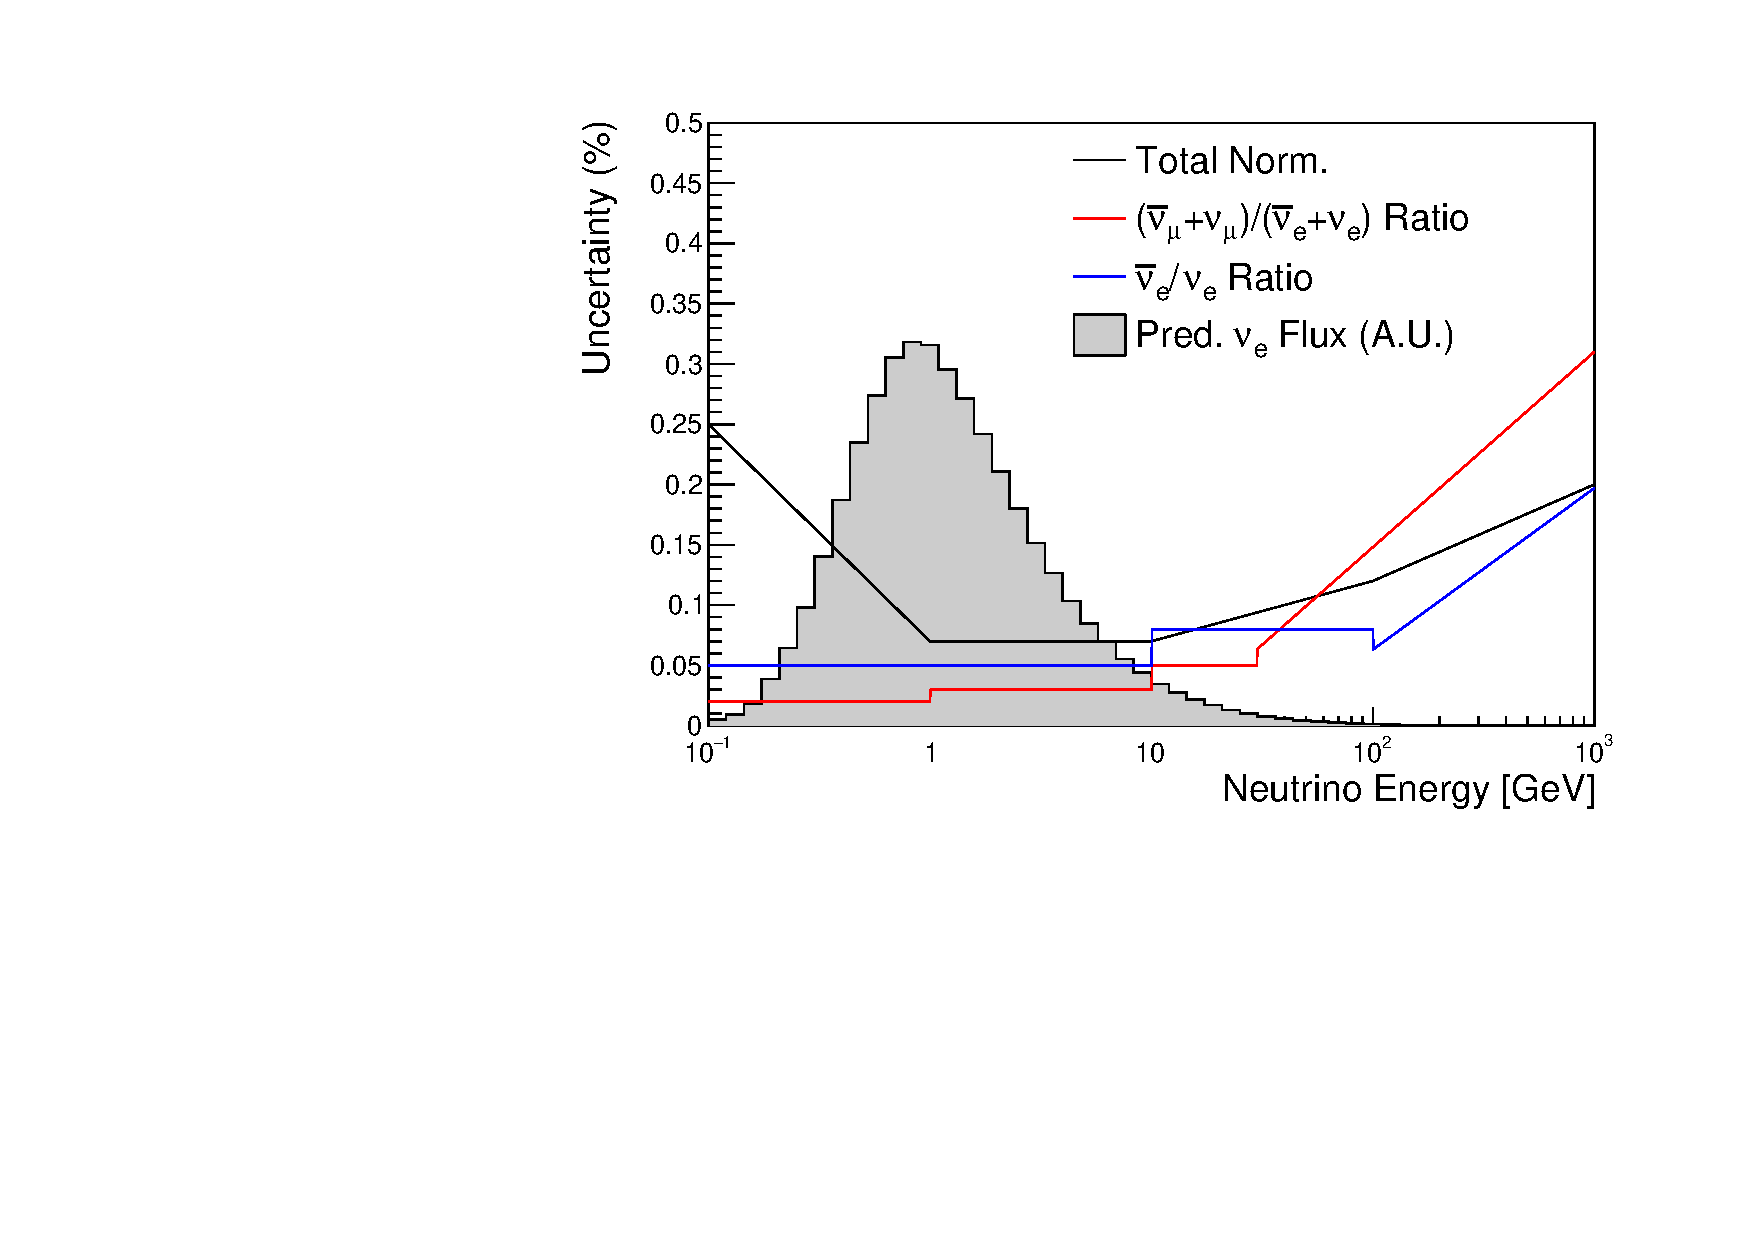
\includegraphics[width=\textwidth, trim={0mm 0mm 0mm 0mm}, clip,page=1]{Figures/Selections/AtmFluxSystSize.pdf}
  \end{subfigure}%
  \begin{subfigure}[t]{0.49\textwidth}
    \includegraphics[width=\textwidth, trim={0mm 0mm 0mm 0mm}, clip,page=3]{Figures/Selections/AtmFluxSystSize.pdf}
  \end{subfigure}
  \caption{The uncertainty evaluated on the atmospheric \quickmath{\nu_{e}} (left) and \quickmath{\nu_{\mu}} (right) flux predictions. The absolute normalisation and flavour ratio uncertainties are given. The solid histogram indicates the neutrino flux as a function of energy.}
  \label{fig:SelsAndSysts_Systs_AtmFluxSysts}
\end{figure}

Updates to the HKKM and Bartol models are underway \cite{Sato2022-ss} to use a similar tuning technique to that used in the beam flux predictions. After those updates, it may be possible to include correlations in the hadron production uncertainty systematics for beam and atmospheric flux predictions.

\subsection{Neutrino Interaction}
\label{sec:SelsAndSysts_Systs_Interaction}

Neutrino interactions in the detectors are modeled by NEUT. The two independent oscillation analyses, T2K-only \cite{t2k_tn_344} and the SK-only \cite{Kamiokande_Collaboration2017-nf}, have developed separate interaction models. To maximise sensitivity out of this simultaneous beam and atmospheric analysis, a correlated interaction model has been defined in \cite{t2k_tn_422}. Where applicable, correlations allow the systematic uncertainties applied to the atmospheric samples to be constrained by near detector neutrino beam measurements. This can lead to stronger sensitivity to oscillation parameters as compared to an uncorrelated model.
%An in-depth discussion of the reasoning and validity of enforcing correlations is documented in \cite{t2k_tn_422} and briefly summarised below.

The low-energy T2K systematic model has a more sophisticated treatment of CCQE, 2p2h, and CCRES uncertainties, where extensive comparisons of this model have been performed to external data \cite{t2k_tn_344}. However, the model is not designed for high-energy atmospheric events, like those illustrated in \autoref{fig:Simulations_NeutrinoEnergyDistribution}. Therefore the high energy systematic model from the SK-only analysis is implemented for the relevant multi-GeV, PC, and up-\quickmath{\mu} samples. The T2K CCQE model is more sophisticated so it has been implemented for all samples within this analysis, where separate low-energy and high-energy dials have been implemented. The low-energy dials are constrained by the near detector measurements and are uncorrelated to their high-energy counterparts. The author of this thesis was responsible for implementing and validating the combined cross-section model as documented in \cite{t2k_tn_422, t2k_tn_426}.

%The CCQE systematic parameters invoked within the SK high energy model are actually contained within T2K's CCQE model. Consequently, the more sophisticated CCQE and CCMEC T2K model parameters have been incorporated into the high energy model but are uncorrelated from the low energy counterparts. 

The high energy systematic model includes parameters developed from comparisons of Nieves and Rein-Seghal models which affect resonant pion producing interactions, comparisons of the GRV98 and CKMT models which control DIS interactions, and hadron multiplicity measurements which modulate the normalisation of multi-pion producing events. The uncertainty on the \quickmath{\nu_{\tau}} cross-section is particularly large and is controlled by a \quickmath{25\%} normalisation uncertainty. These uncertainties are applied via normalisation or shape parameters. The former linearly scales the weight of all affected Monte-Carlo events, whereas the latter can increase or decrease a particular event's weight depending on its neutrino energy and mode of interaction. The response of the shape parameters is defined by third-order polynomial splines which return a weight for a particular neutrino energy. To reduce computational resources for the far detector fit, the response is binned by neutrino energy and sample binning: lepton momentum and cosine zenith binning for atmospheric splined responses and reconstructed neutrino energy and direction binning for beam samples. In total, \quickmath{17} normalisation and \quickmath{15} shape parameters are included in the high-energy model within this analysis.

\autoref{fig:SelsAndSysts_NeutrinoEnergyComparison} indicates the predicted neutrino energy distribution for both beam and subGeV atmospheric samples. There is clearly significant overlap in neutrino energy between the subGeV atmospheric and beam samples, allowing similar kinematics in the final state particles. \autoref{fig:SelsAndSysts_FractionalModeComparison} illustrates the fractional contribution of the different interaction modes per sample.

Comparing beam and atmospheric samples which target CCQE interactions (\texttt{S.G. e-like 0de}, \texttt{S.G. \quickmath{\mu}-like [0,1]de}, \texttt{[FHC,RHC]1R \quickmath{\mu}-like} and \texttt{[FHC,RHC]1R e-like} samples), there is a very similar contribution of CCQE, CC 2p2h, and CC\quickmath{1\pi^{\pm}} interactions. The samples which target CC\quickmath{1\pi^{\pm}} interactions, (\texttt{S.G. e-like 0de}, \texttt{S.G. \quickmath{\mu}-like 2de} and \texttt{FHC 1R+1d.e e-like}) also consist of very similar mode interactions.

As a consequence of the similarity in energy and mode contributions, correlating the systematic model between the beam and subGeV atmospheric samples ensures that this analysis attains the largest sensitivity to oscillation parameters while still ensuring neutrino interaction systematics are correctly accounted for. Due to its more sophisticated CCQE and 2p2h model, the T2K systematic model was chosen as the basis of the correlated model. 

\begin{figure}[h]
  \begin{subfigure}[t]{0.49\textwidth}
    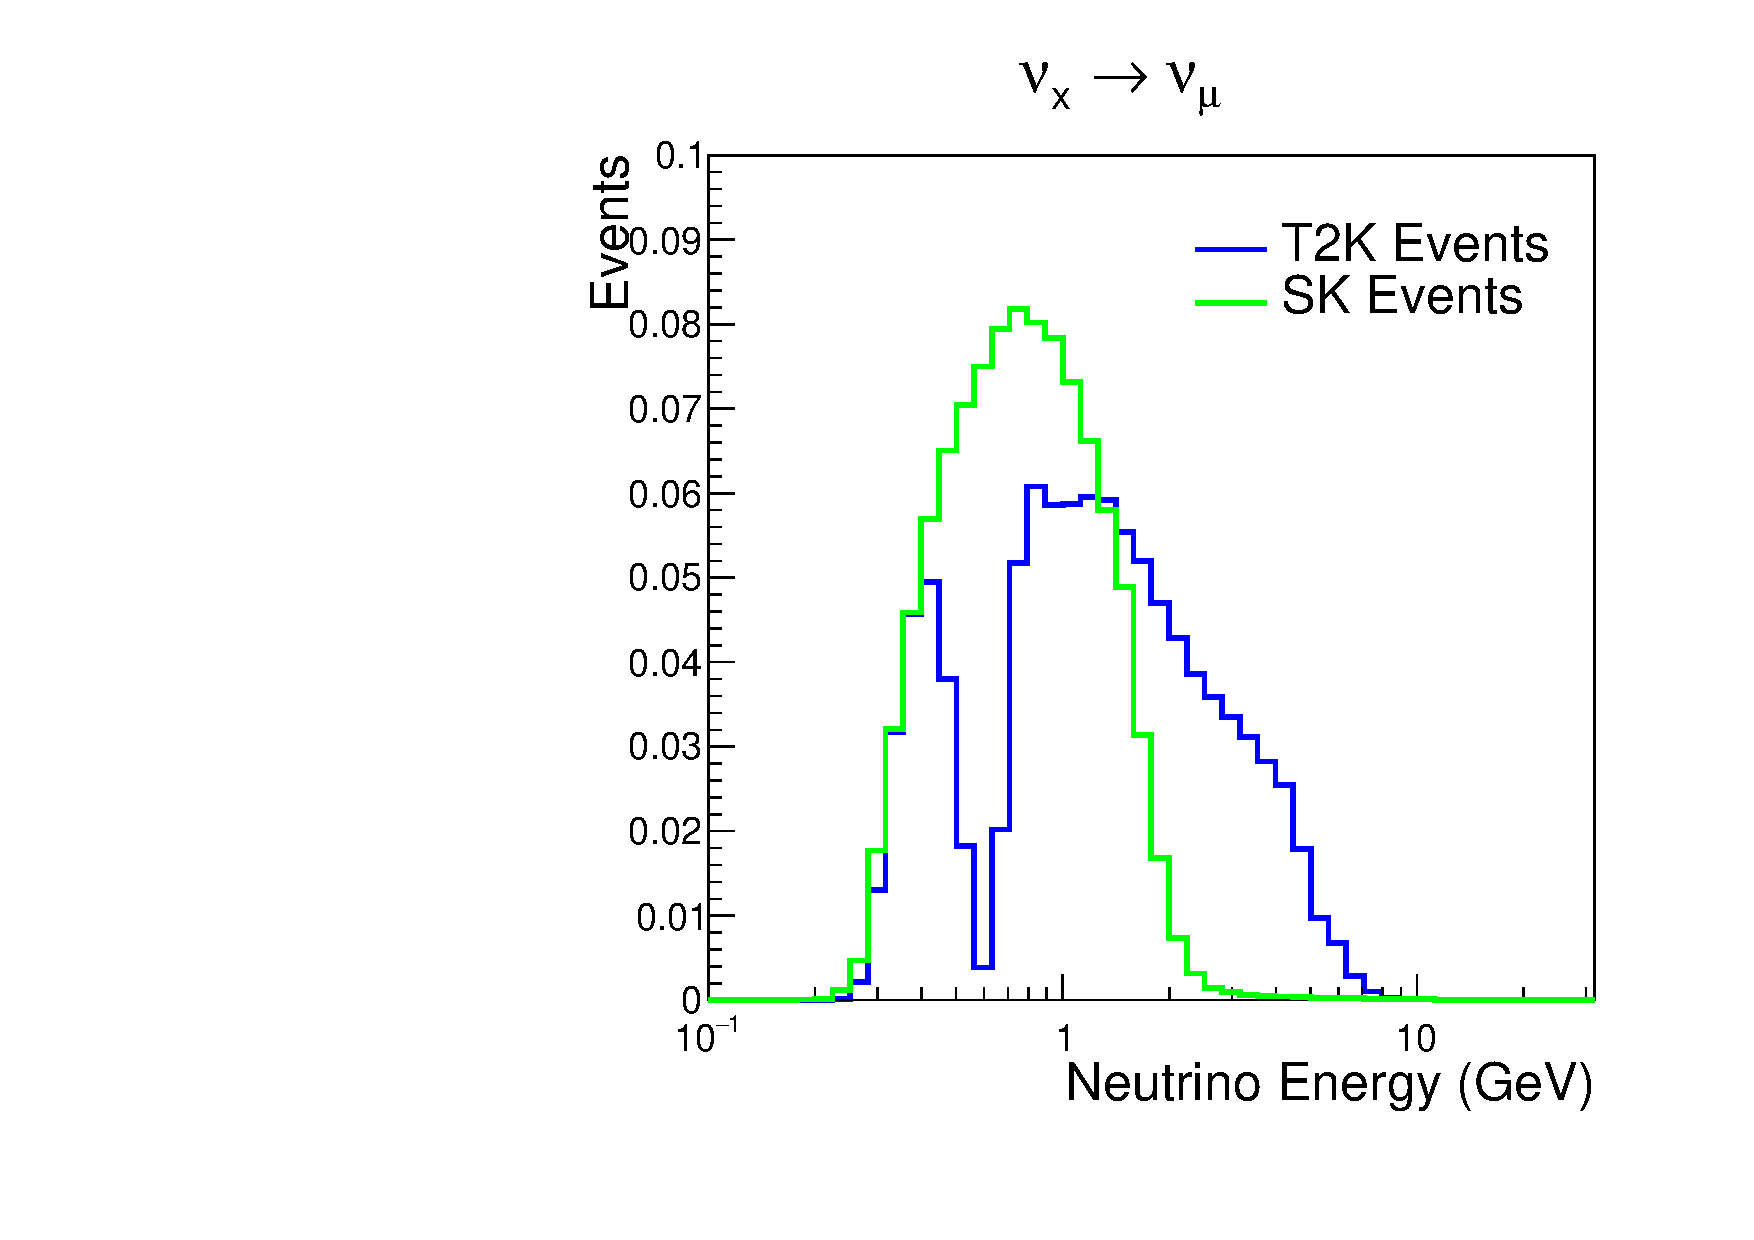
\includegraphics[width=\textwidth, trim={0mm 0mm 0mm 0mm}, clip,page=1]{Figures/Selections/NeutrinoEnergyDist_Comp_1Rmu_NuMu.pdf}
    \subcaption{\quickmath{\mu}-like}
  \end{subfigure}%
  \begin{subfigure}[t]{0.49\textwidth}
    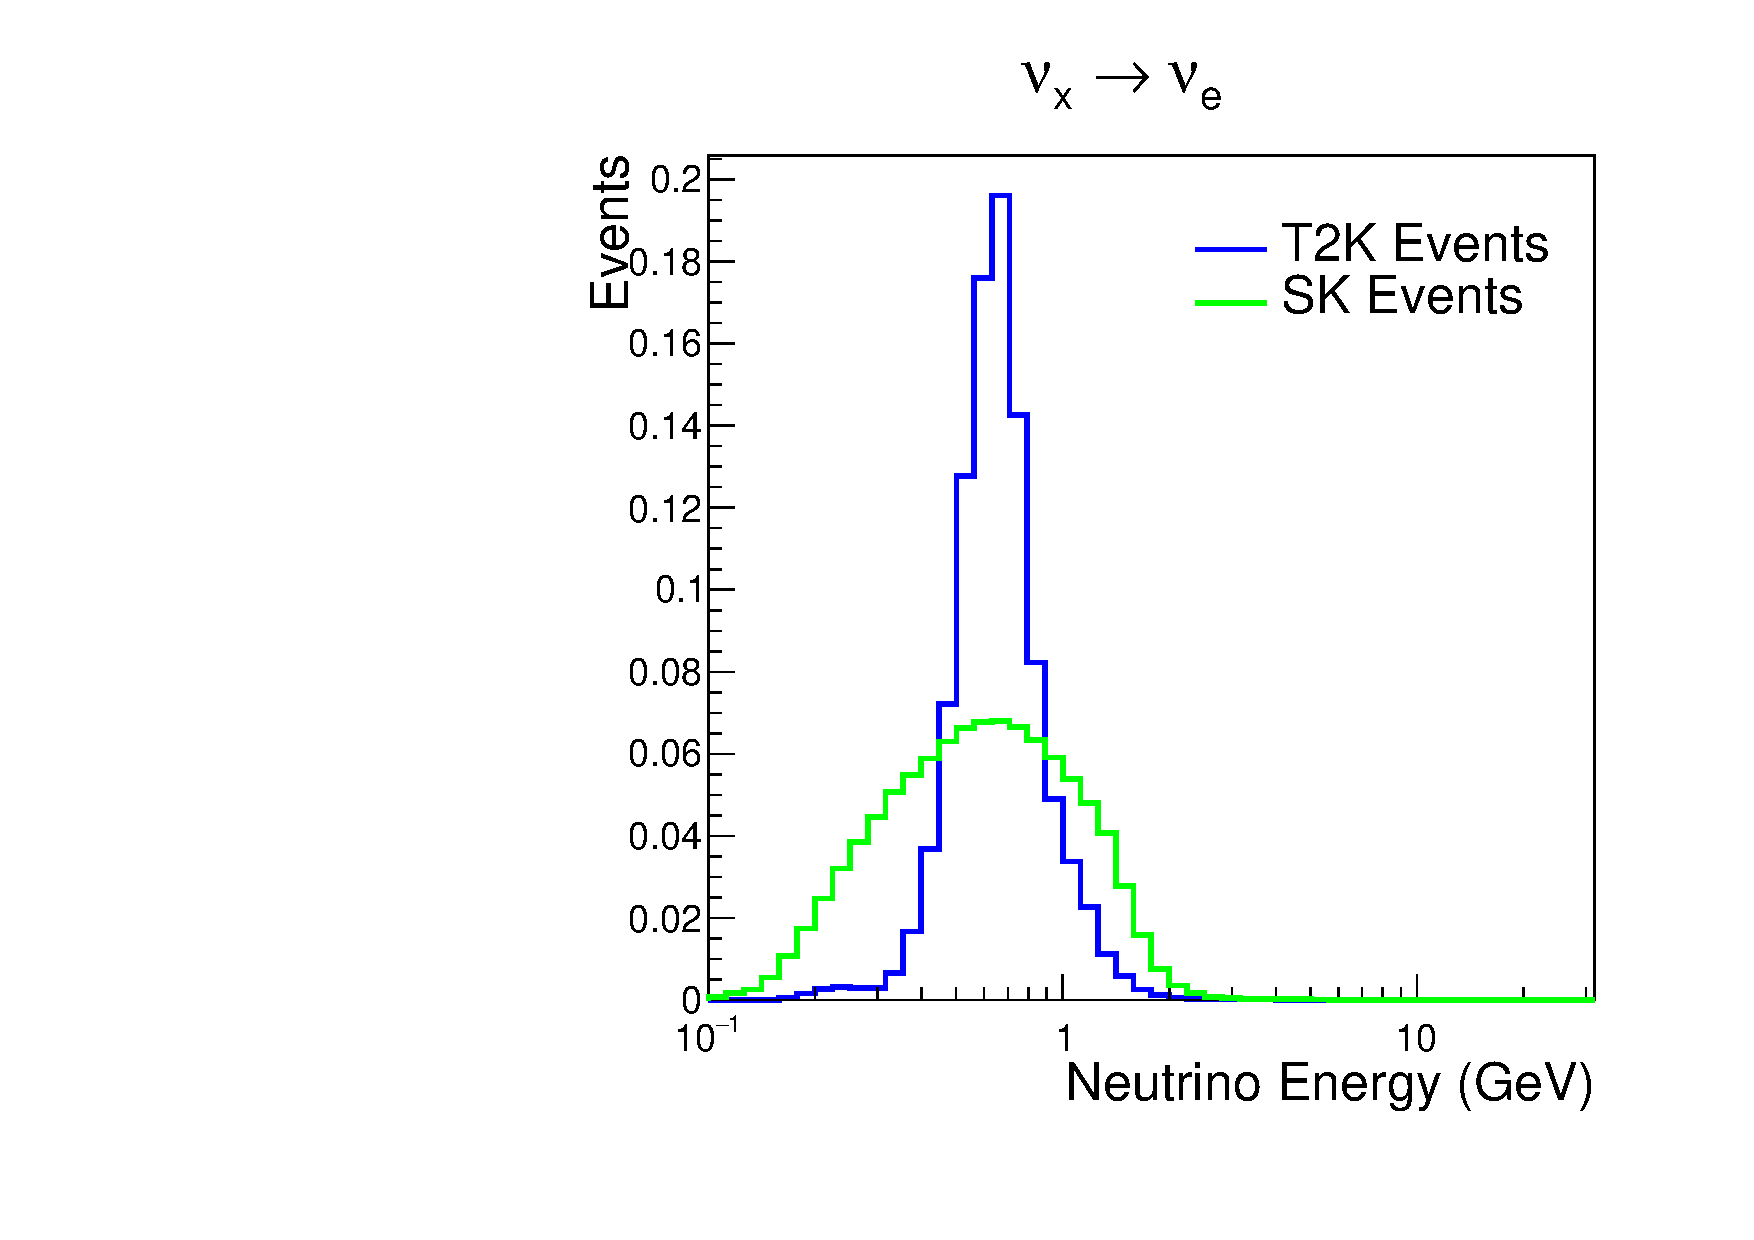
\includegraphics[width=\textwidth, trim={0mm 0mm 0mm 0mm}, clip,page=1]{Figures/Selections/NeutrinoEnergyDist_Comp_1Re_NuE.pdf}
    \subcaption{\quickmath{e}-like}
  \end{subfigure}
  \begin{subfigure}[t]{0.49\textwidth}
    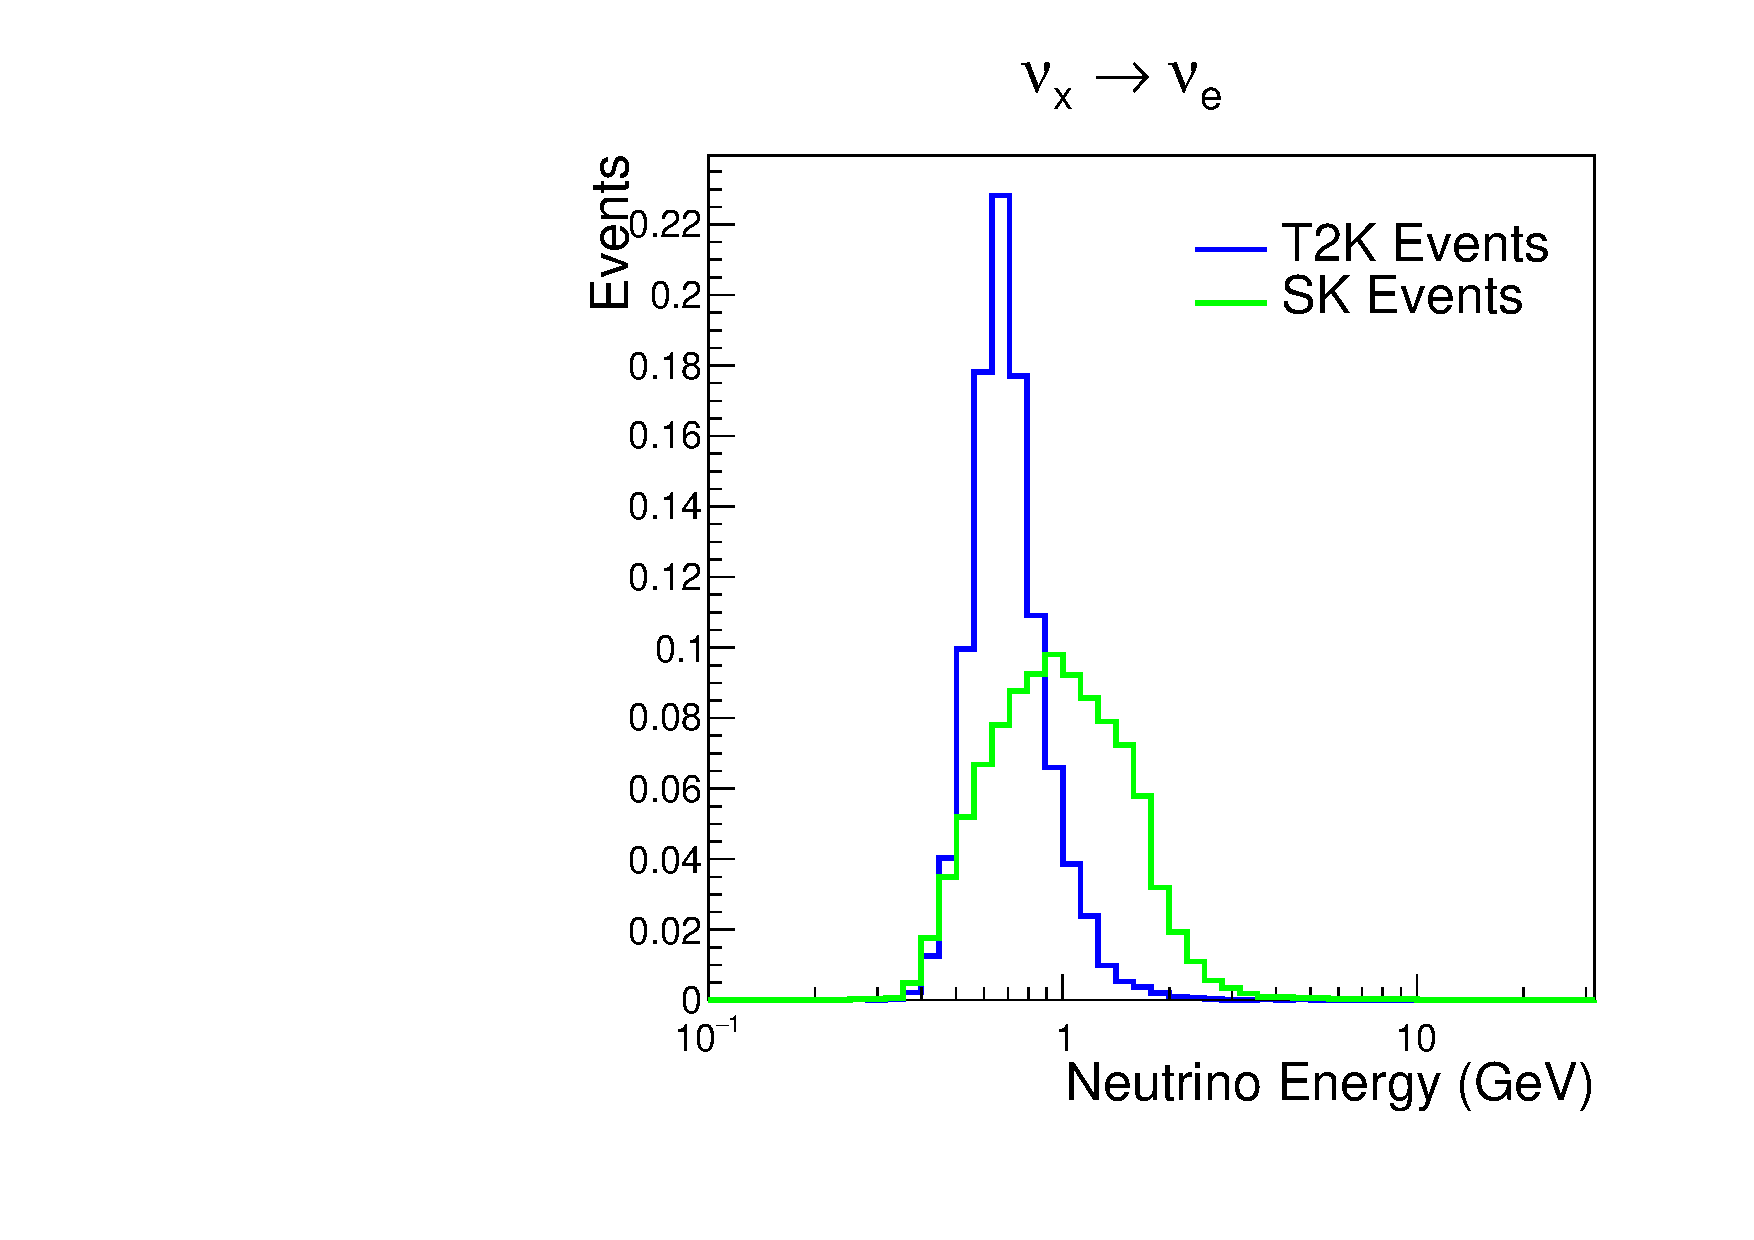
\includegraphics[width=\textwidth, trim={0mm 0mm 0mm 0mm}, clip,page=1]{Figures/Selections/NeutrinoEnergyDist_Comp_1Re1de_NuE.pdf}
    \subcaption{\quickmath{e}-like + 1d.e.}
  \end{subfigure}
  \caption{The predicted neutrino energy distribution for subGeV atmospheric and beam samples. FHC and RHC beam samples are summed together Asimov A oscillation parameters are assumed (given in \autoref{tab:Theory_ParameterSets}). Beam and atmospheric samples with similar cuts are compared against one another.}
  \label{fig:SelsAndSysts_NeutrinoEnergyComparison}
\end{figure}

\begin{figure}[h]
  \begin{subfigure}[t]{\textwidth}
    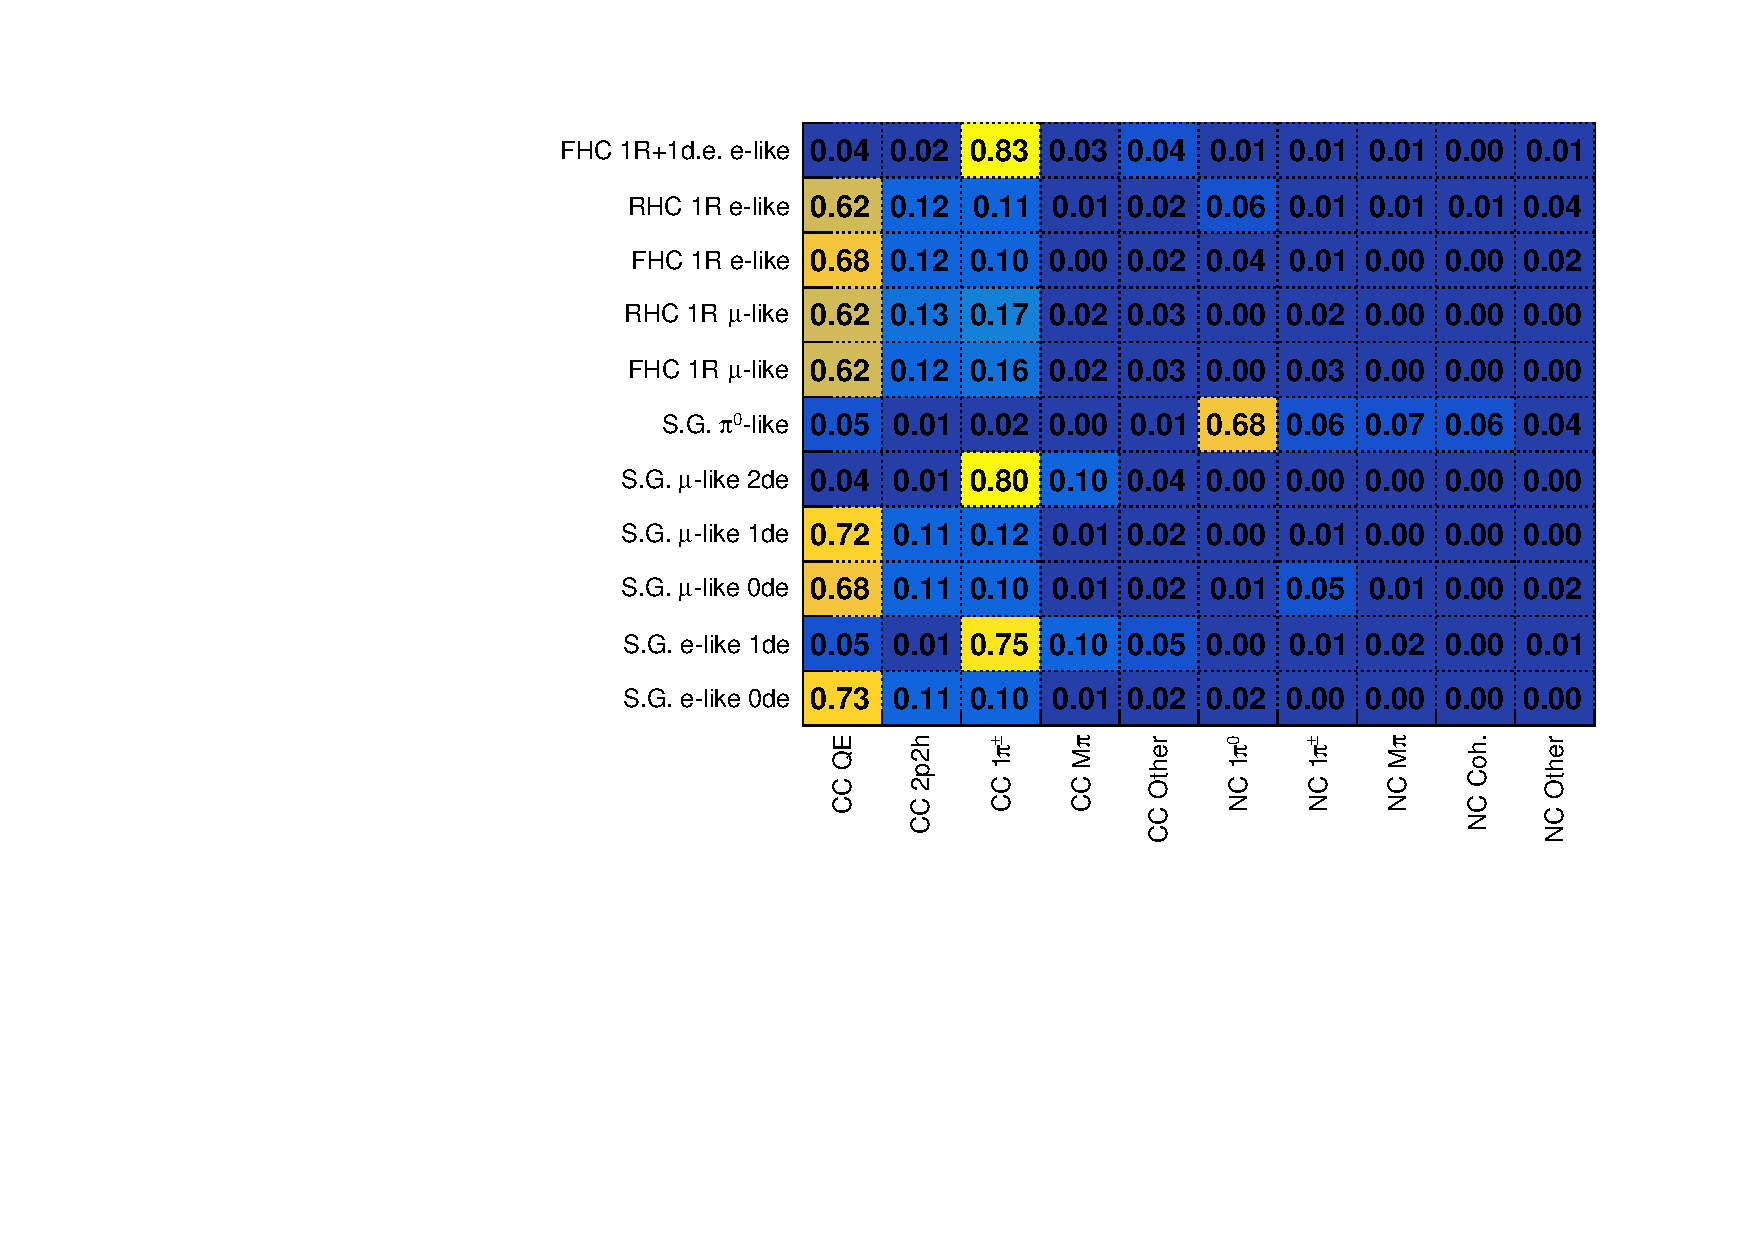
\includegraphics[width=\textwidth, trim={0mm 0mm 0mm 0mm}, clip,page=1]{Figures/Selections/FractionalModeComparison.pdf}
  \end{subfigure}
  \caption{The interaction mode contribution of each sample given as a fraction of the total event rate in that sample. Asimov A oscillation parameters are assumed (given in \autoref{tab:Theory_ParameterSets}). The Charged Current (CC) modes are broken into quasi-elastic (QE), 2p2h, resonant charged pion production (\quickmath{1\pi^{\pm}}), multi-pion production (\quickmath{M\pi}), and other interaction categories. Neutral Current (NC) interaction modes are given in interaction mode categories: \quickmath{\pi^{0}} production, resonant charged pion production,  multi-pion production, and others.}
  \label{fig:SelsAndSysts_FractionalModeComparison}
\end{figure}

The T2K systematic model \cite{t2k_tn_344} is applied in a similar methodology to the SK model parameters. It consists of \quickmath{19} shape parameters and \quickmath{24} normalisation parameters. Four additional parameters, which model the uncertainty in the binding energy, are applied in a way to shift the momentum of the lepton emitted from a nucleus. This controls the uncertainty specified on the \quickmath{27\text{MeV}} binding energy assumed within \autoref{sec:SelsAndSysts_Erec_CCQE}. The majority of these parameters are assigned a Gaussian prior uncertainty. Those that have no reasonably motivated uncertainty, or those which have not been fit to external data, are assigned a flat prior which does not affect the penalty term.

%The CCQE model parameters were tuned to MiniBooNE \cite{miniboone_nu_ccqe} and MINER\quickmath{\nu}A \cite{minerva_nubar_ccqe} measurements and CCRES model parameters are tuned to ANL and BNL experiments \cite{ANL_BNL_corr}.

On top of the combination of the SK and T2K interaction models, several other parameters have been specifically developed for the joint oscillation analysis. The majority of the atmospheric samples' \quickmath{\delta_{CP}} sensitivity comes from the normalisation of subGeV electron-like events. These are modeled using a spectral function to approximate the nuclear ground state. However, the near detector is not able to constrain the model so an additional systematic is introduced which models an alternative Continous Random Phase Approximation (CRPA) nuclear ground state. This dial approximates the event weights if a CRPA model had been assumed rather than a spectral function. This dial only applies to \quickmath{\nu_{e}} and \quickmath{\bar{\nu}_{e}} as the near detector does not constraint \quickmath{\nu_{e}} cross-section measurements. It is applied as a shape parameter.

Further additions to the model have been introduced due to the inclusion of the subGeV \quickmath{\pi^{0}} atmospheric sample. This particularly targets charged current and neutral current \quickmath{\pi^{0}} producing interactions to help constrain the systematic uncertainties. Therefore, an uncertainty that affects neutral current resonant \quickmath{\pi^{0}} production is incorporated into this analysis. Comparisons of NEUT's NC resonant pion production predictions have been made to MiniBooNE \cite{MB_NC1pi0} data and a consistent \quickmath{16\%} to \quickmath{21\%} underprediction is observed \cite{t2k_tn_422}. Consequently, a conservative \quickmath{30\%} normalisation parameter is invoked. 

Down-going events are mostly insensitive to oscillation parameters and can act similar to the near detector within an accelerator experiment (Details will be discussed in \autoref{chap:OscillationProbability}). This region of phase space can act as a sideband and allows the cross-section model and near detector constraint to be studied. The distribution of events in this region is calculated using the technique outlined in \autoref{sec:MarkovChainMonteCarlo_Predictives}. The results are illustrated in \autoref{fig:SelsAndSysts_DownGoingPredictives}. For CCQE-targeting samples, the application of the near detector constraint is well within the statistical fluctuation of the down-going data. This means there is no significant tension is observed between the data and the Monte Carlo prediction after the near detector constraint is applied. This is not the case for samples with target CCRES interactions. The electron-like data is consistent with the constrained prediction at high reconstructed momenta but diverges at lower momentum, whereas the muon-like sample is under-predicted throughout the range of momenta. To combat this disagreement, an additional cross-section systematic dial, specifically designed to inflate the low pion momentum systematics was developed in \cite{t2k_tn_422}. This is a shape parameter implemented through a splined response. 

\begin{figure}[h]
  \begin{subfigure}[t]{0.49\textwidth}
    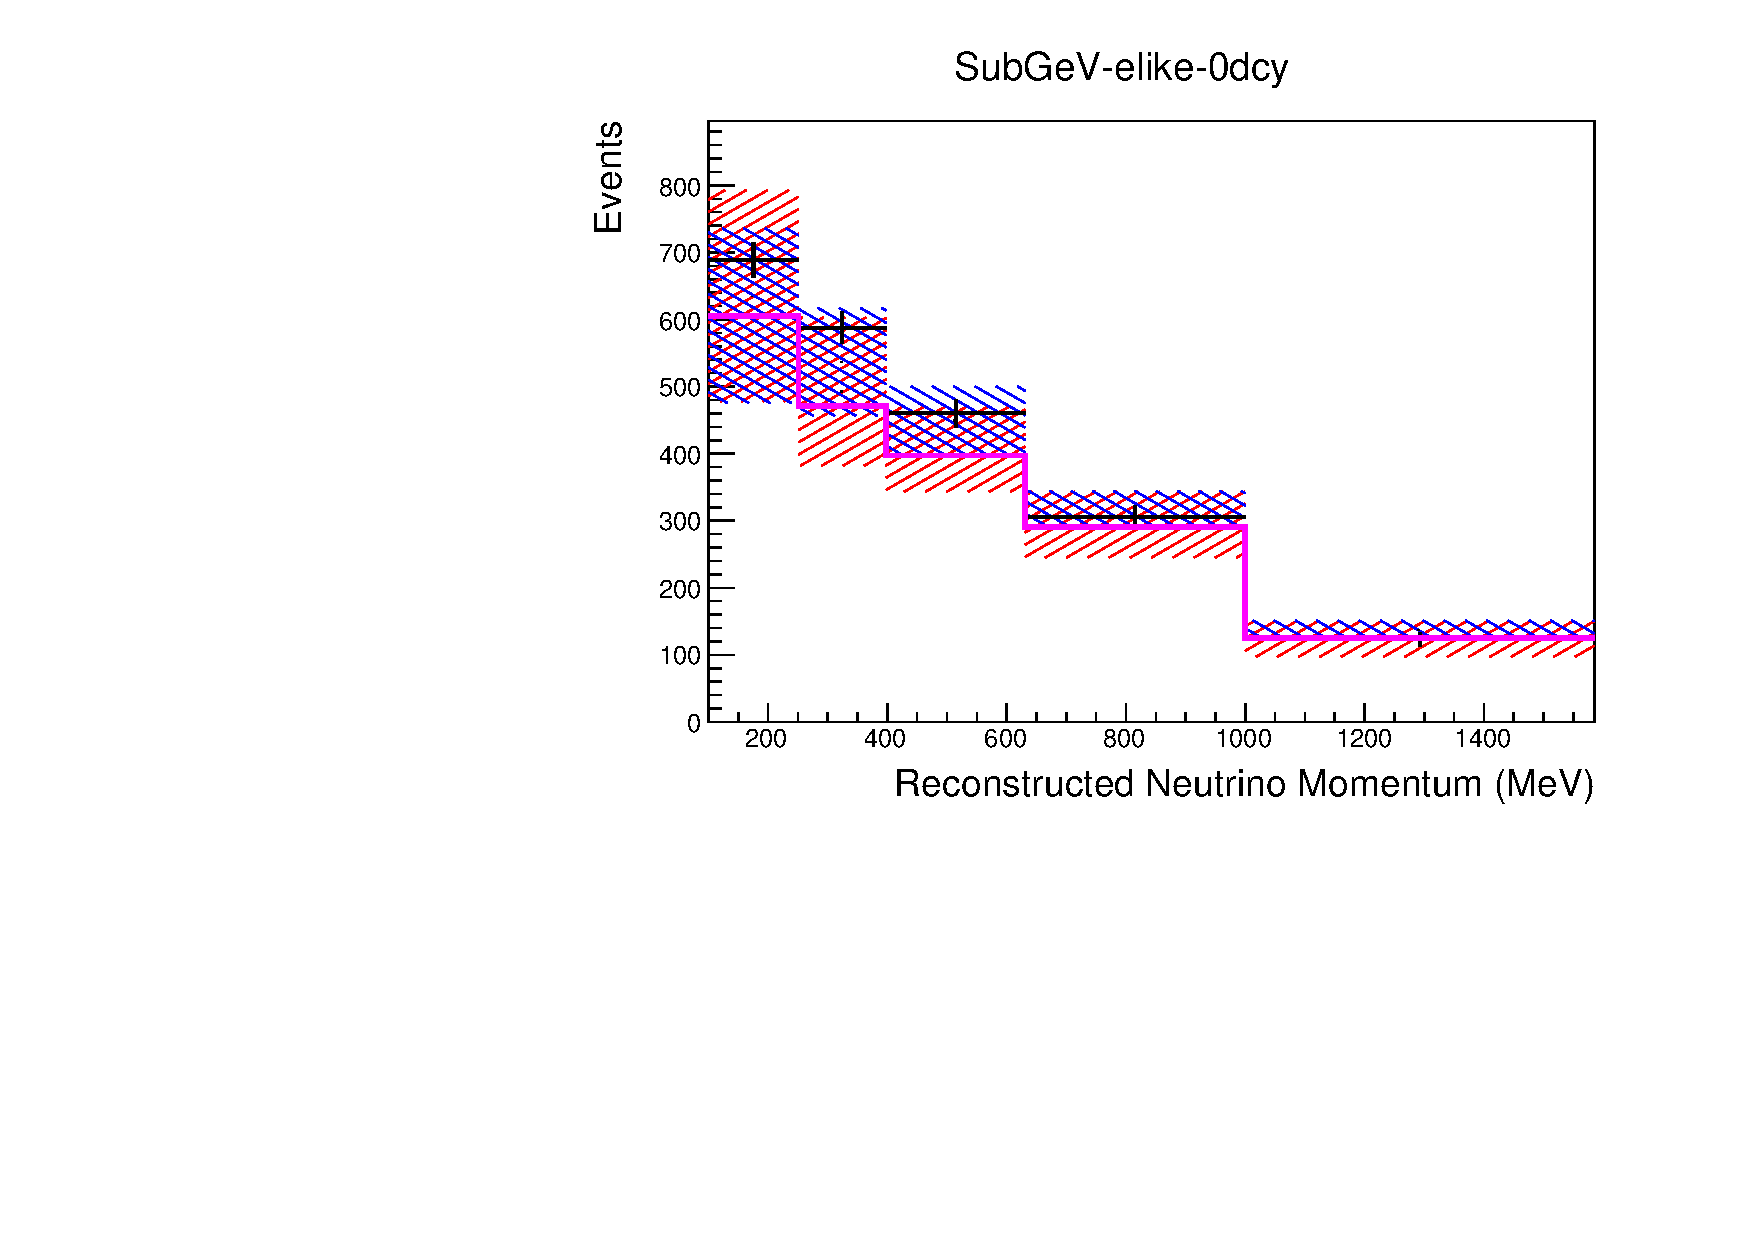
\includegraphics[width=\textwidth, trim={0mm 0mm 0mm 0mm}, clip,page=1]{Figures/Selections/Predictive_SubGeV-elike-0dcy.pdf}
  \end{subfigure}%
  \begin{subfigure}[t]{0.49\textwidth}
    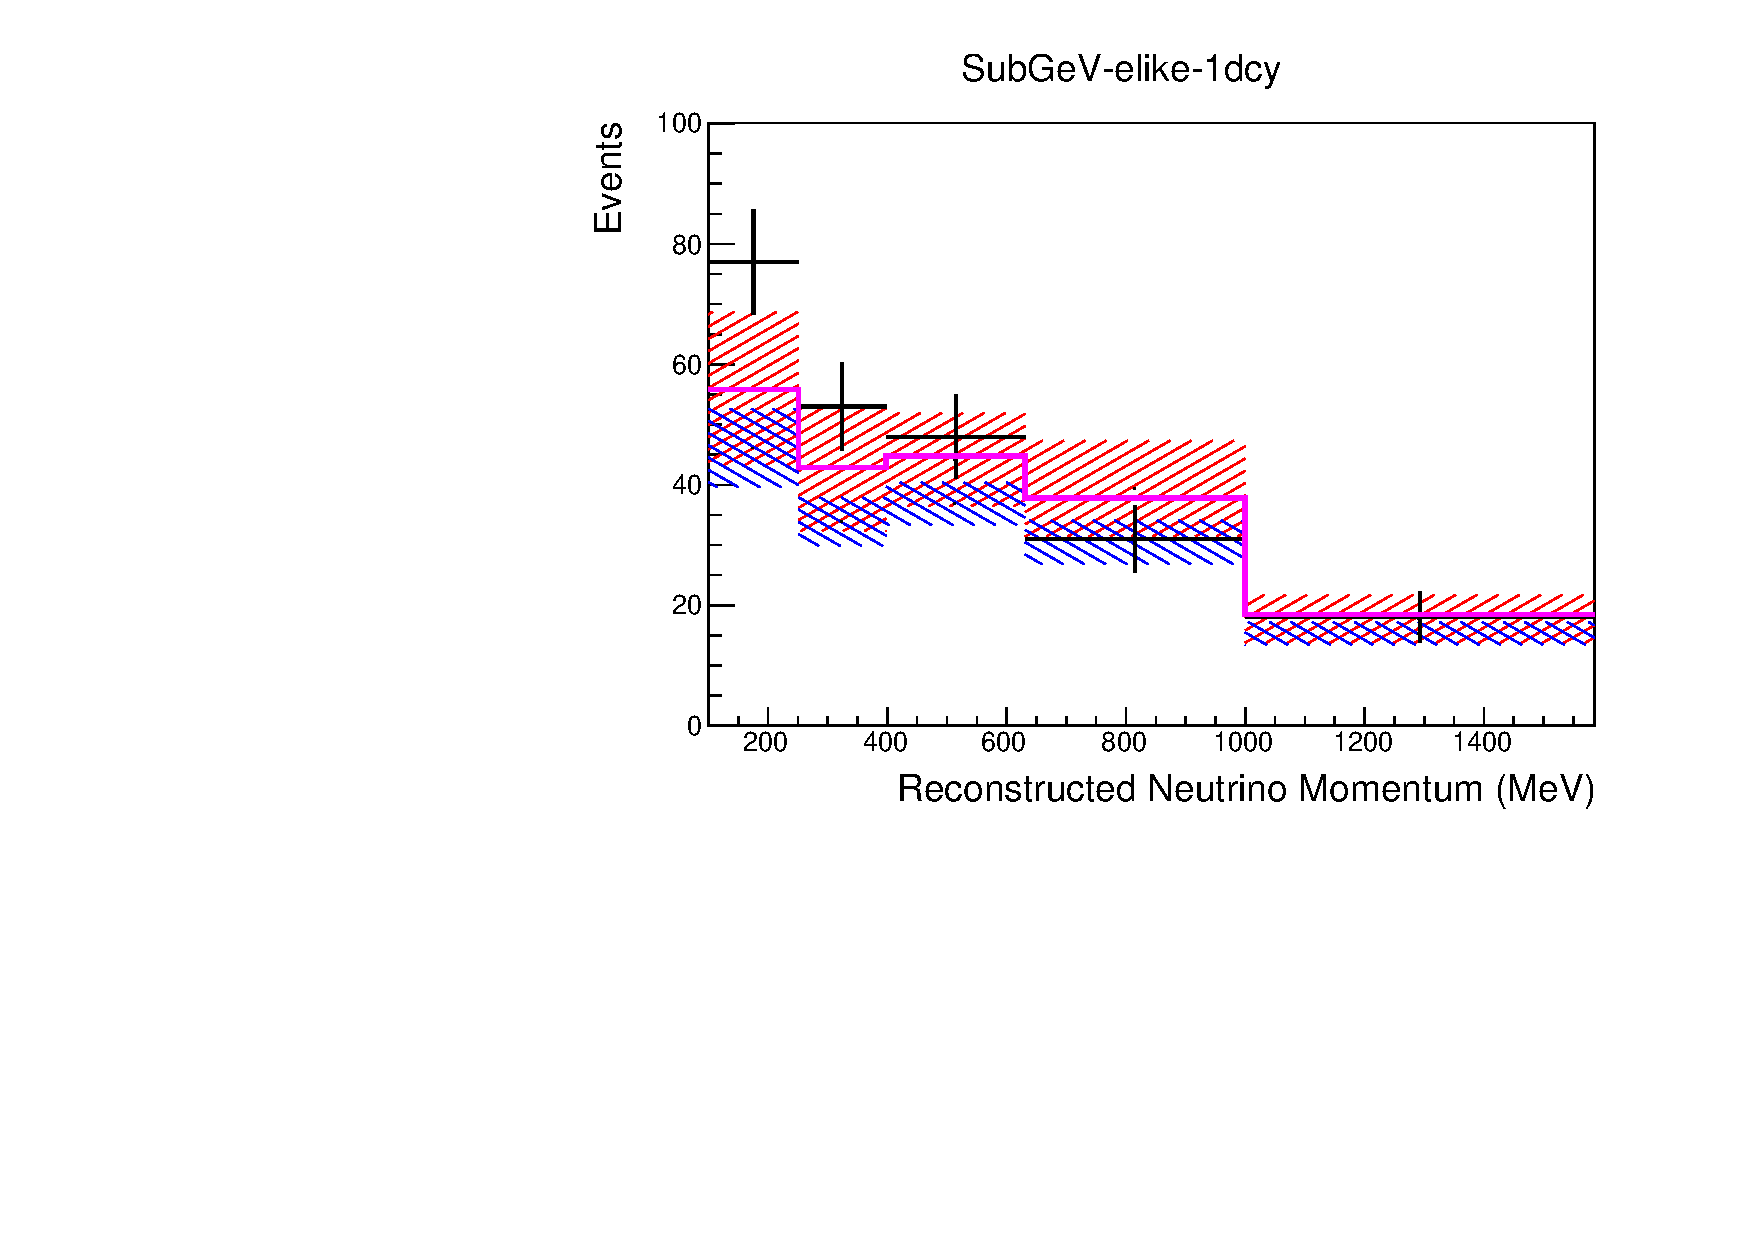
\includegraphics[width=\textwidth, trim={0mm 0mm 0mm 0mm}, clip,page=1]{Figures/Selections/Predictive_SubGeV-elike-1dcy.pdf}
  \end{subfigure}
  \begin{subfigure}[t]{0.49\textwidth}
    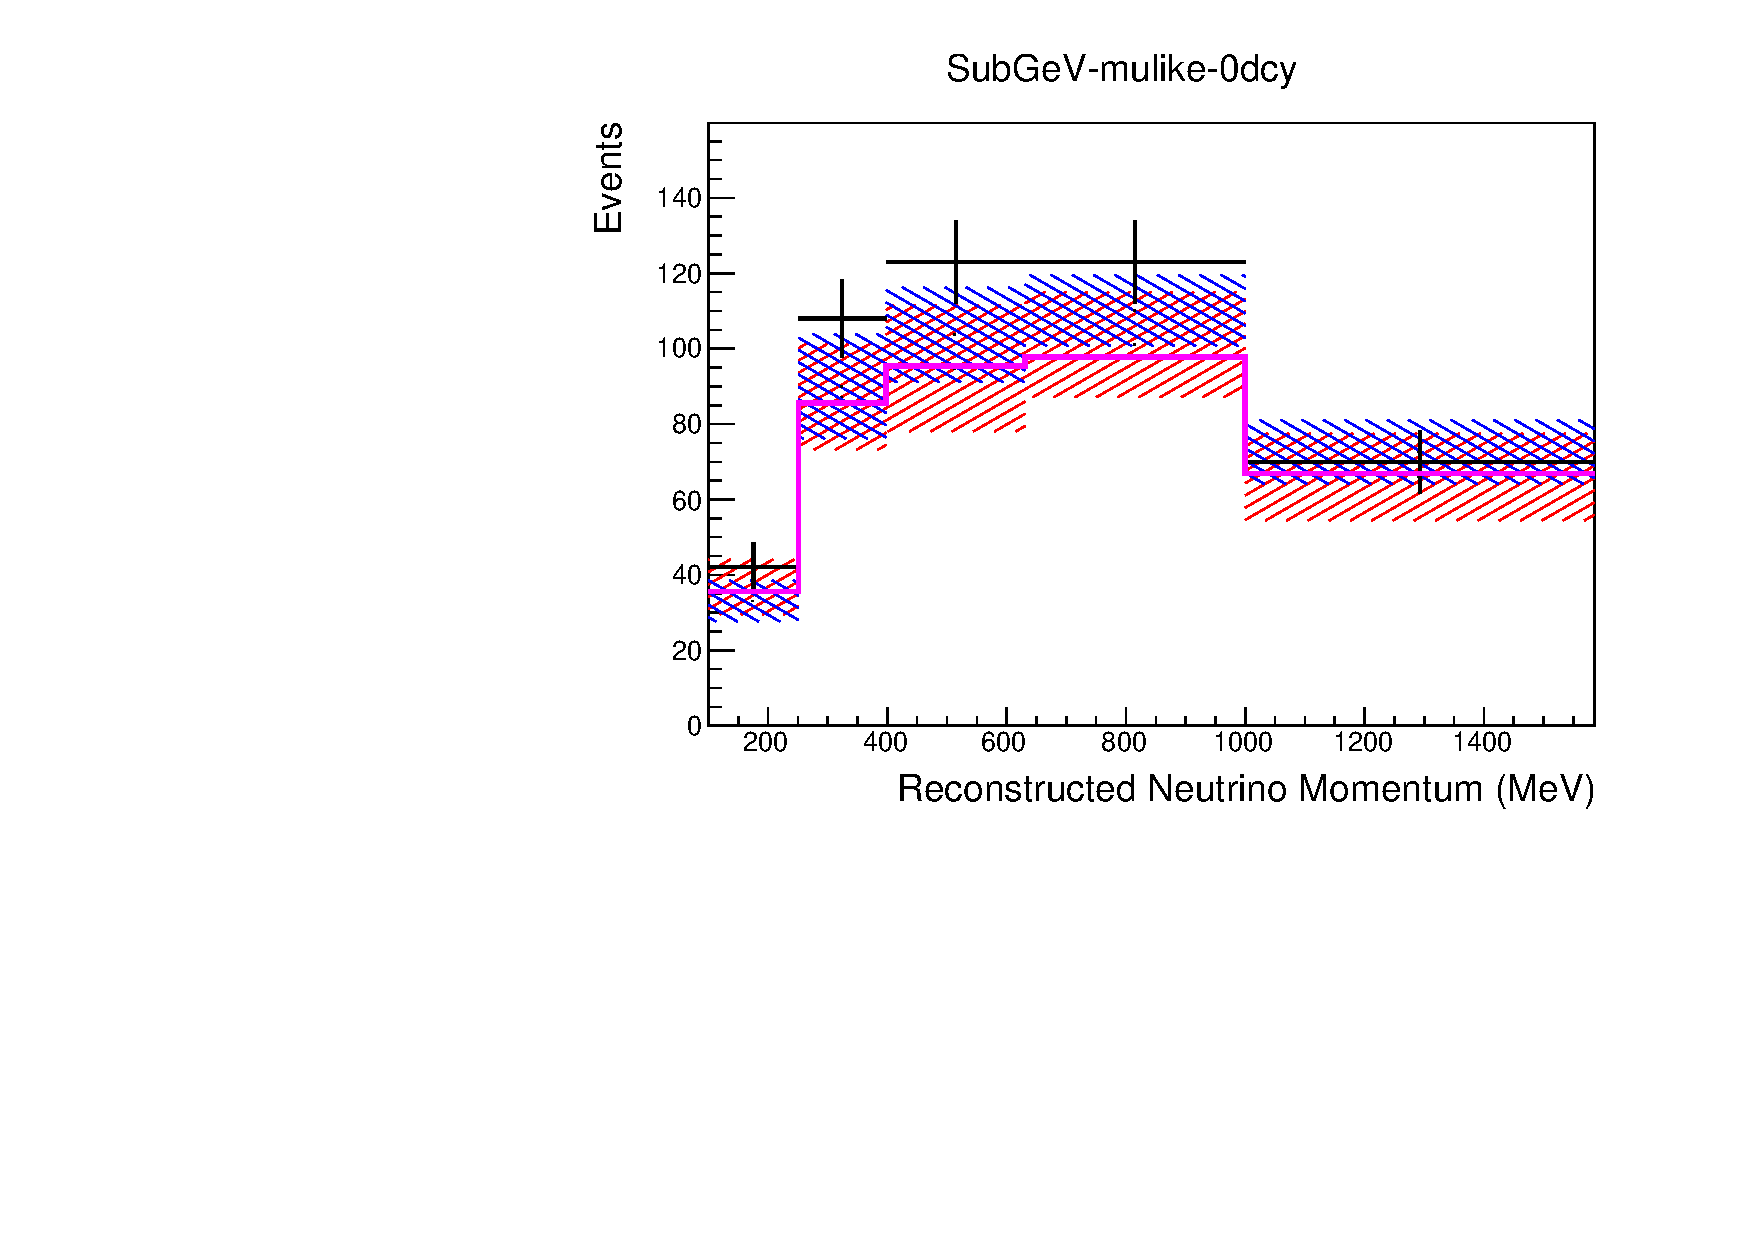
\includegraphics[width=\textwidth, trim={0mm 0mm 0mm 0mm}, clip,page=1]{Figures/Selections/Predictive_SubGeV-mulike-0dcy.pdf}
  \end{subfigure}%
  \begin{subfigure}[t]{0.49\textwidth}
    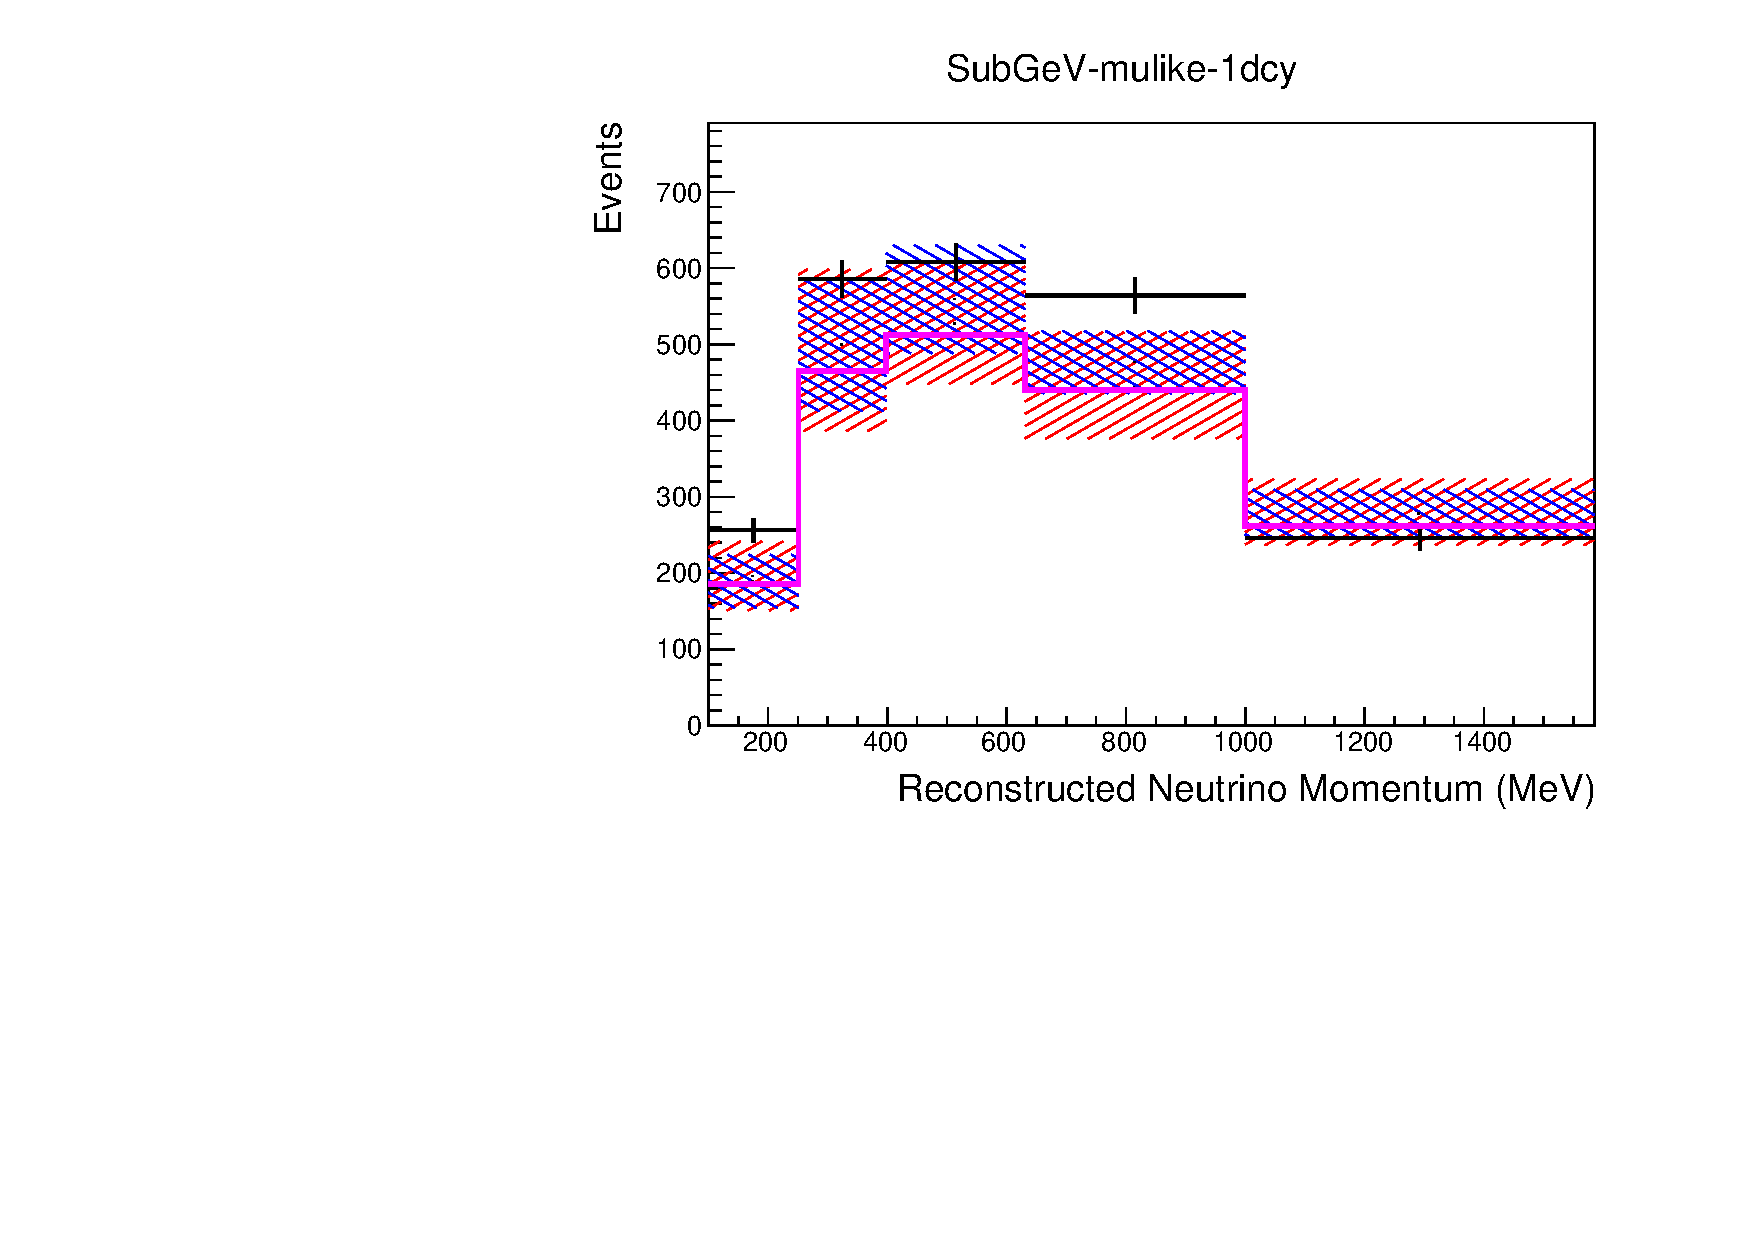
\includegraphics[width=\textwidth, trim={0mm 0mm 0mm 0mm}, clip,page=1]{Figures/Selections/Predictive_SubGeV-mulike-1dcy.pdf}
  \end{subfigure}
  \begin{subfigure}[t]{0.49\textwidth}
    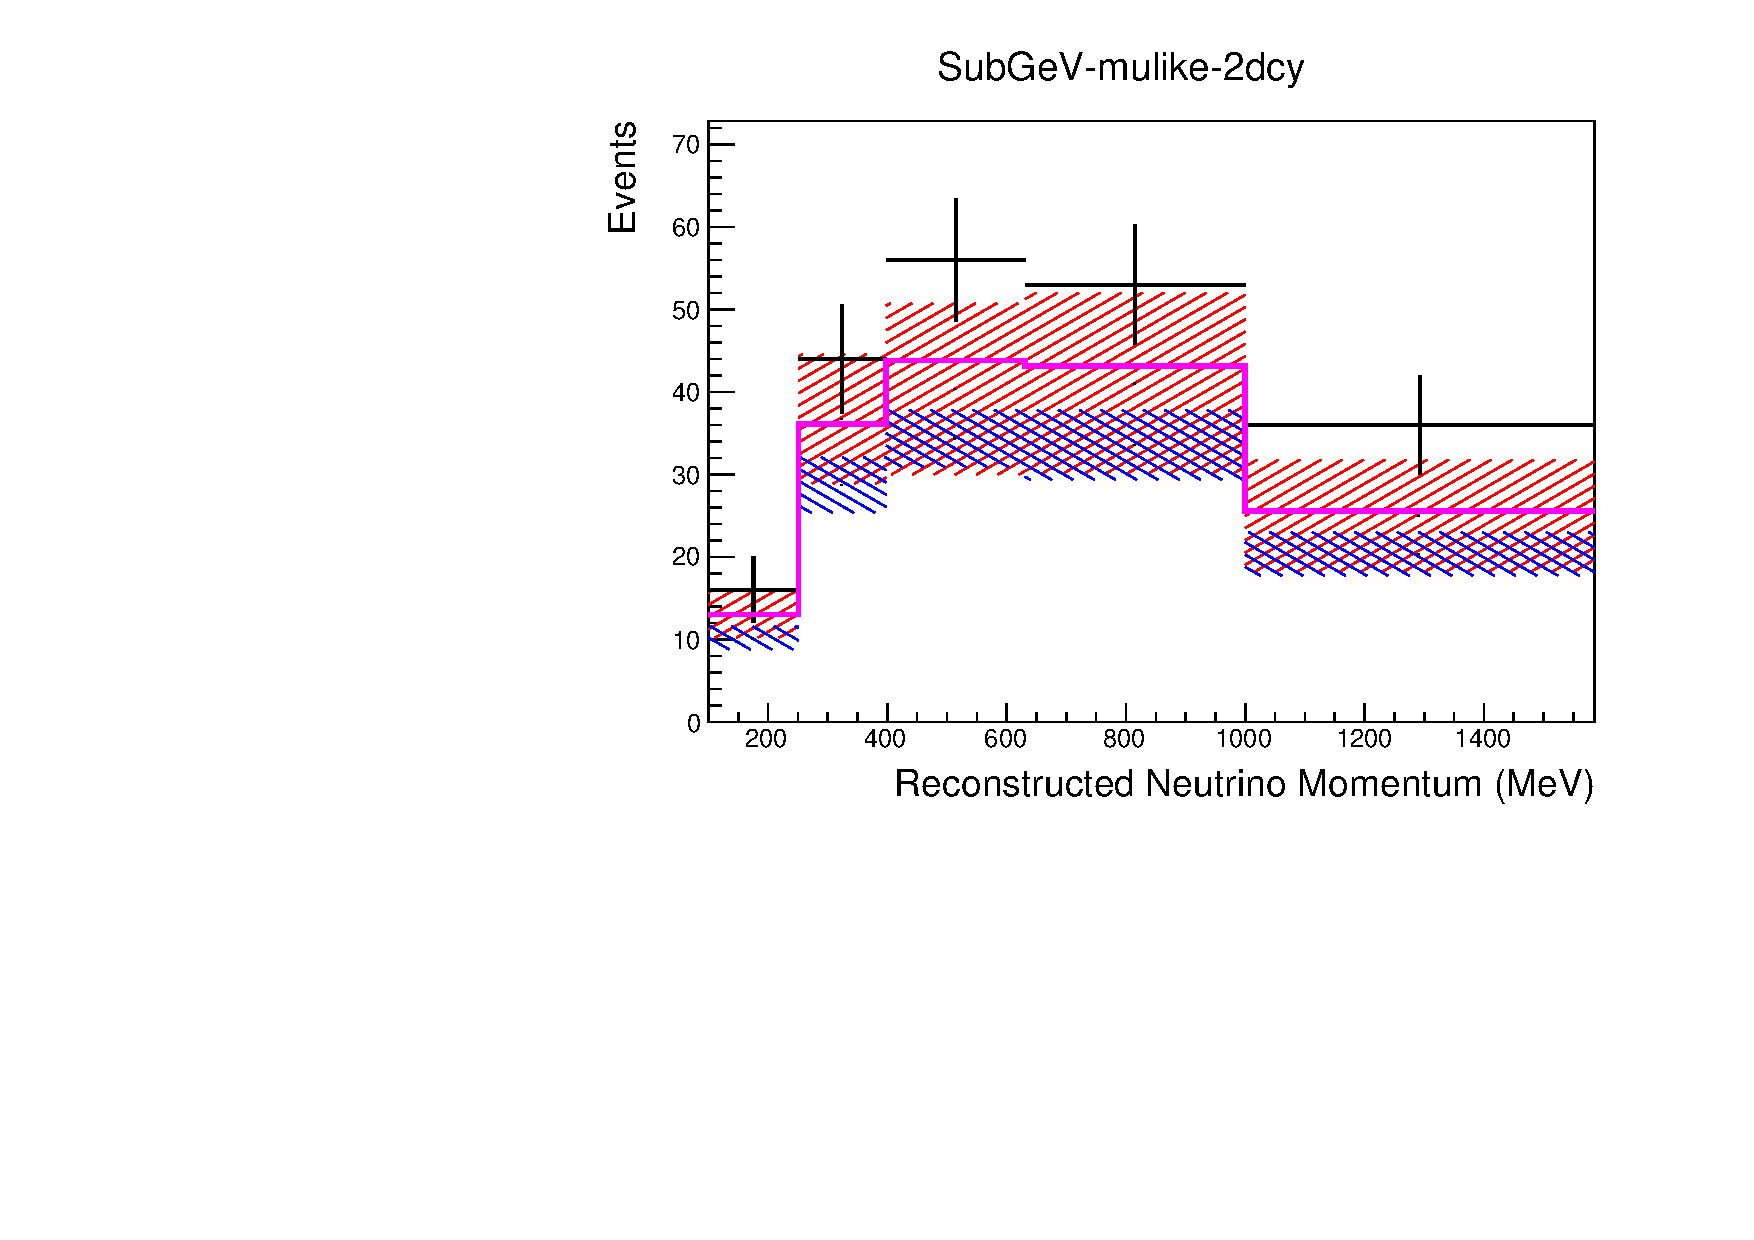
\includegraphics[width=\textwidth, trim={0mm 0mm 0mm 0mm}, clip,page=1]{Figures/Selections/Predictive_SubGeV-mulike-2dcy.pdf}
  \end{subfigure}
  \caption{Down-going atmospheric subGeV single-ring samples comparing the mean and error of the pre-fit and post-fit Monte Carlo predictions in red and blue, respectively. The magenta histogram illustrates the Monte Carlo prediction using the generated dial values. The black points illustrate the down-going data with statistical errors given. The mean and errors of the Monte Carlo predictions are calculated by the techniques documented in \autoref{sec:MarkovChainMonteCarlo_Predictives}. The pre-fit spectrum is calculated by throwing the cross-section and atmospheric flux dial values from the pre-fit covariance matrix. The post-fit spectrum is calculated by sampling the cross-section dial values from an ND fit MCMC chain, whilst still throwing the atmospheric flux dials from the pre-fit covariance.}
  \label{fig:SelsAndSysts_DownGoingPredictives}
\end{figure}

\subsection{Near Detector}
\label{sec:SelsAndSysts_Systs_ND}

The systematics applied due to uncertainties arising from the response of the near detector is documented in \cite{thesis_clarence}. The response is described by \quickmath{574} normalisation parameters binned in the selected sample as well as momentum and angle, \quickmath{P_{\mu}} and \quickmath{\cos(\theta_{\mu})}, of the final-state muon. These are applied via a covariance matrix with each parameter being assigned a Gaussian prior from that covariance matrix. These normalisation parameters are built from underlying systematics, e.g. pion secondary interaction systematics, which are randomly thrown and the variation in each \quickmath{P_{\mu} \times \cos(\theta_{\mu})} bin is determined. Two thousand throws are evaluated and a covariance matrix response is created. This allows significant correlations between FGD1 and FGD2 samples, as well as adjacent \quickmath{P_{\mu} \times \cos(\theta_{\mu})} bins. Statistical uncertainties are accounted for by including fluctuations of each event's weight from a Poisson distribution.

Similar to the cross-section systematics, MaCh3 and BANFF are used to constrain the uncertainty of these systematics through independent validations. Each fitter generates a post-fit covariance matrix which is compared and passed to the far-detector oscillation analysis working group. As the analysis presented within this thesis uses the \texttt{MaCh3} framework, a joint oscillation analysis fit of all three sets of samples and their respective systematics is performed.

\subsection{Far Detector}
\label{sec:SelsAndSysts_Systs_FD}

Two configurations of the far detector systematic model implementation have been considered. Firstly, the far detector systematic uncertainties for beam and atmospheric samples are taken from their respective analysis inputs, denoted ``official inputs'' analysis, with no correlations assumed between the beam and atmospheric samples. The beam- and atmospheric-specific inputs are documented in \autoref{sec:SelsAndSysts_Systs_FDBeam} and \autoref{sec:SelsAndSysts_Systs_FDAtm}. Secondly, an alternative detector model has been developed which correlates the response of the SK detector systematics between the beam and atmospheric samples. Here, the distribution of parameters used for applying event cuts (e.g. electron-muon PID separation) is modified within the fit. It follows a similar methodology to the beam far detector systematics implementation but performs a joint fit of the beam and atmospheric data. This alternative implementation is detailed in \autoref{sec:SelsAndSysts_Systs_Correlated}.

\subsubsection{Beam Samples}
\label{sec:SelsAndSysts_Systs_FDBeam}

%There are \quickmath{45} systematics which describes the response of the far detector, specifically for beam sample neutrino events. \quickmath{44} of these parameters are normalisation parameters and are split by the interaction mode, true neutrino flavour, reconstructed neutrino energy, and sample which they affect. The final parameter is the energy scale uncertainty. It is applied as a multiplicative factor to the reconstructed neutrino energy. The value of the systematic is taken from Monte Carlo to data differences illustrated in \cite{sk_2017}. 

There are \quickmath{45} systematics which describe the response of the far detector to beam events \cite{t2k_tn_399}, split into \quickmath{44} normalisation parameters and one energy scale systematic. The energy scale systematic is applied as a multiplicative scaling of the reconstructed neutrino energy. It is estimated from data-to-Monte Carlo differences in the stopping muon sample in \cite{sk_2017} and found to be \quickmath{2.1\%}. The normalisation parameters are assigned a Gaussian error centered at one with width taken from a covariance matrix. A detailed breakdown of the generation of the covariance matrix is found in \cite{t2k_tn_318}. To build the covariance matrix, a fit is performed on atmospheric data which has been selected using beam sample selection cuts. These cuts use the variables, \quickmath{L^{i}}, where the index \quickmath{i} is detailed in \autoref{tab:SelsAndSysts_Systs_CutVariables}. Each \quickmath{L^{i}} is a smear, \quickmath{\alpha}, and shift, \quickmath{\beta} parameter such that,

\begin{equation}
  \label{eqn:SelsAndSysts_Systs_ShiftSmear}
  L^{i}_{j} \rightarrow \bar{L}^{i}_{j} = \alpha^{i}_{j} L + \beta^{i}_{j}
\end{equation}

Where \quickmath{L^{i}_{j}} (\quickmath{\bar{L}^{i}_{j}}) correspond to nominal(varied) PID cut parameters given in \autoref{tab:SelsAndSysts_Systs_CutVariables}. The shift and smear parameters are nuisance parameters with no prior constraints. They are binned by final-state topology, \quickmath{j}, where the binning is given in \autoref{tab:SelsAndSysts_Systs_Topologies}. The final-state topology binning is because the detector will respond differently to events that have one or multiple rings. For example, the detector will be able to distinguish single-ring events better than two overlapping ring events, resulting in different systematic uncertainty for one-ring events compared to two-ring events. This approach is used to allow the cut parameter distributions to be modified within the fit, allowing for better data to Monte Carlo agreement. %Only the shape of each of the cut variables is used within this fit, such that physics effects are not considered.

\begin{table}[ht!]
    \centering
    \begin{tabular}{c|l}
      \hline
      Cut Variable & Parameter Name \\
      \hline
      \quickmath{0} & \texttt{fiTQun} \quickmath{e/\mu} PID \\
      \quickmath{1} & \texttt{fiTQun} \quickmath{e/\pi^{0}} PID \\
      \quickmath{2} & \texttt{fiTQun} \quickmath{\mu/\pi} PID \\
      \quickmath{3} & \texttt{fiTQun} Ring-Counting Parameter \\
      \hline
      \hline
    \end{tabular}
    \caption{List of cut variables that are included within the shift/smear fit documented in \cite{t2k_tn_318}.}      
    \label{tab:SelsAndSysts_Systs_CutVariables}
\end{table}

\begin{table}[ht!]
  \centering
  \begin{tabular}{c|l}
    \hline
    Category & Description \\
    \hline
    \quickmath{1e} & Only one electron above Cherenkov threshold in the final state \\
    \quickmath{1\mu} & Only one muon above Cherenkov threshold in the final state \\
    \quickmath{1e\text{+other}} & One electron and one or more other charged particles above \\
    & \hspace{0.2cm}Cherenkov threshold in the final state \\
    \quickmath{1\mu\text{+other}} & One muon and one or more other charged particles above \\
    & \hspace{0.2cm}Cherenkov threshold in the final state \\
    \quickmath{1\pi^0} & Only one $\pi^0$ in the final state\\
    \quickmath{1\pi^\pm} or \quickmath{1\text{p}} & Only one hadron (typically charged pion or proton) in the final state\\
    Other & Any other final state\\
    \hline
  \end{tabular}
  \caption{Reconstructed event topology categories on which the SK detector systematics \cite{t2k_tn_318} are based.}
  \label{tab:SelsAndSysts_Systs_Topologies}
\end{table}

The mis-modeling of \quickmath{\pi^{0}} events is also considered. If one of the two rings from a \quickmath{\pi^{0}} event is missed, this will be reconstructed as a CC\quickmath{\nu_{e}}-like event. This is one of the largest systematics hindering the electron neutrino appearance analyses. Consequently, additional systematics have been introduced to constrain the mis-modeling of \quickmath{\pi^{0}} events in SK, binned by reconstructed neutrino energy. To evaluate this systematic uncertainty, a set of ``hybrid-\quickmath{\pi^{0}}'' samples is constructed. These events are built by overlaying one electron-like ring from the SK atmospheric neutrino samples or decay electron ring from a stopping cosmic ray muon with one simulated photon ring. Both rings are chosen so that momenta and opening angle follow the decay kinematics of NC \quickmath{\pi^0} events from the T2K-MC. Hybrid-\quickmath{\pi^{0}} Monte Carlo samples with both rings from the SK Monte Carlo are produced to compare with the hybrid-\quickmath{\pi^{0}} data samples and the difference in the fraction of events that pass the \quickmath{\nu_{e}} selection criteria is used to assign the systematic errors. In order to investigate any data to Monte Carlo differences that may originate from either the higher energy ring or lower energy ring, two samples are built; a sample in which the electron constitutes the higher energy ring from the \quickmath{\pi^{0}} decay (called the primary sample) and another one in which it constitutes the lower energy ring (called the secondary sample). The standard T2K \quickmath{\nu_{e}} fiTQun event selection criteria are used to select events.

Final contributions to the covariance matrix are determined by supplementary uncertainties obtained by comparing stopping muon data to Monte Carlo prediction, as first introduced in \autoref{sec:Simulation_Reconstruction}. The efficiency of tagging decay electrons is estimated by the stopping muon data to Monte Carlo differences by comparing the number of one decay electron events to the number of events with one or fewer decay electrons. Similarly, the rate at which fake decay electrons are reconstructed by \texttt{fiTQun} is estimated by comparing the number of two decay electron events to the number of events with one or two reconstructed decay electrons. The two sources of systematics are added in quadrature weighted by the number of events with one true decay electron yielding a \quickmath{0.2\%} systematic uncertainty.
%The muon misidentification rate is estimated by comparing the number of electron-like events which have one decay electron to the total number of events with one decay electron. This systematic is estimated as a \quickmath{30\%} effect in the rate of muon misidentification.
A fiducial volume systematic of \quickmath{\pm 2.5\text{cm}} which corresponds to a \quickmath{0.5\%} shift in the normalisation of events is also applied. Additional normalisation uncertainties based on neutrino flavour and interaction mode are also defined in \cite{t2k_tn_399, t2k_tn_186, t2k_tn_107}.

Two additional sources of uncertainty are included: secondary and photo-nuclear interactions. These are estimated by varying the underlying parameters are building a distribution of sample event rates. These contributions are then added in quadrature to the above covariance matrix. The final uncertainty on the SK detector systematics are provided in \autoref{fig:SelsAndSysts_SKCovDiagonals}. 

\begin{figure}[h]
  \begin{subfigure}[t]{0.9\textwidth}
    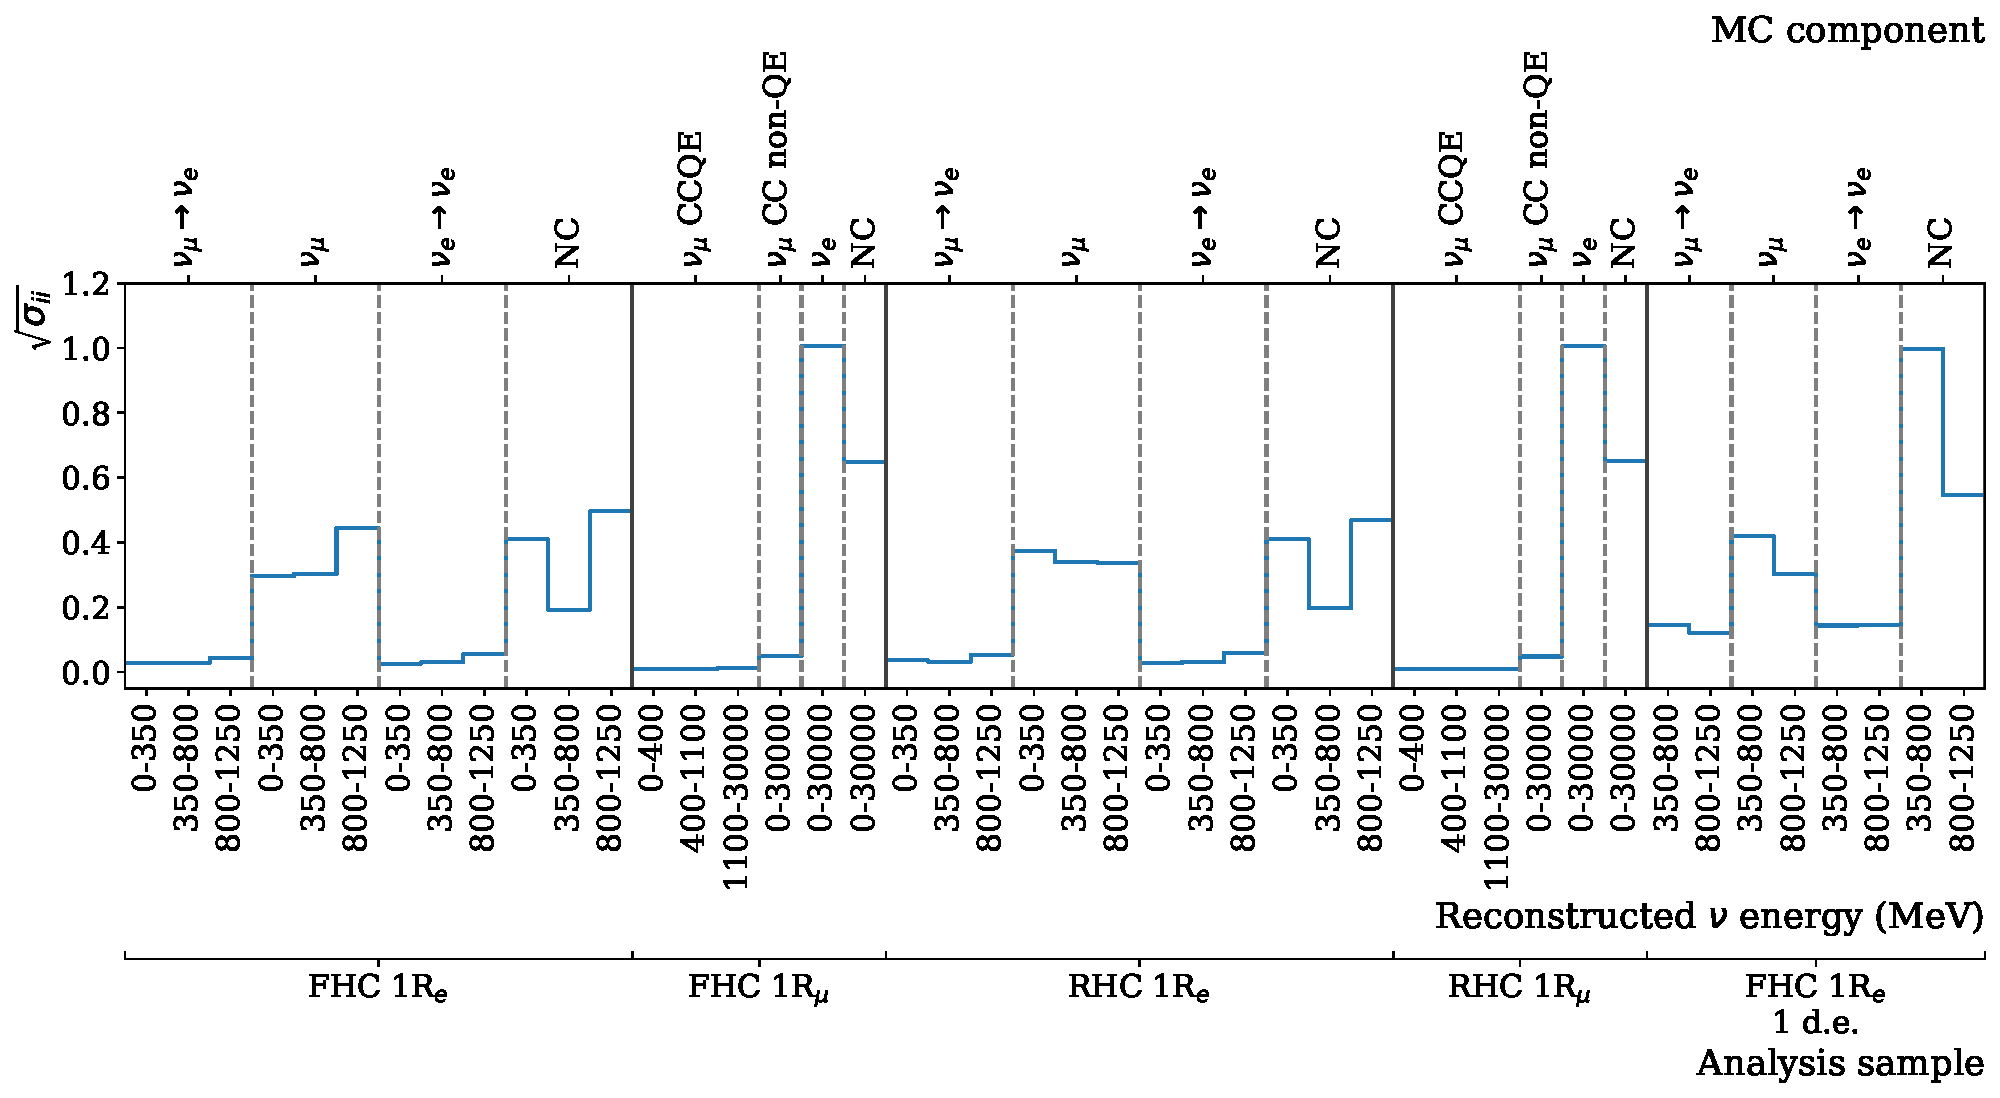
\includegraphics[width=\textwidth, trim={0mm 0mm 0mm 0mm}, clip,page=1]{Figures/Selections/SK_Error_2020_Erec.pdf}
  \end{subfigure}
  \caption{The uncertainty on each of the 44 parameters describing the SK detector systematics (The energy scale systematic is neglected). The parameters are split by sample, oscillation channel, interaction mode and reconstructed neutrino energy.}
  \label{fig:SelsAndSysts_SKCovDiagonals}
\end{figure}

\subsubsection{Atmospheric Samples}
\label{sec:SelsAndSysts_Systs_FDAtm}

The detector systematics for atmospheric samples, documented in \cite{Jiang2019-iw}, are split into two sub-groups: those which are related to particle identification and ring counting systematics, and those which are related to calibration, separation, and reduction uncertainties.

The particle identification systematics consist of five parameters. The ring separation systematic enforces an anti-correlated response between the single-ring and multi-ring samples. This is implemented as a fractional increase/decrease in the overall normalisation of each sample, depending on the distance to the nearest wall from an event's vertex. The coefficients of the normalisation are estimated prior to the fit and depend on the particular atmospheric sample. Two electron-muon separation systematics are included within this model which anti-correlates the response of the electron-like and muon-like samples: one for single-ring events and another for multi-ring events.

The multi-ring electron-like separation likelihood, discussed in \autoref{sec:SelsAndSysts_Sels_Atms}, encodes the ability of the detector to separate neutrino from anti-neutrino events. Two normalisation parameters vary the relative normalisation of multi-ring \quickmath{\nu_e} and \quickmath{\bar{\nu}_e} samples whilst keeping a consistent overall event rate.

There are 22 systematics related to calibration measurements, including effects from backgrounds, reduction, and showering effects. They are documented in \cite{Jiang2019-iw} and are briefly summarised in \autoref{SelsAndSysts_Systs_ATMPDCalibSysts}. They are applied via normalisation parameters, with the separation systematics requiring the conservation of event rate across all samples.

\begin{table}[ht!]
  \centering
  \caption{Sources of systematic errors specified within the grouped into the ``calibration'' systematics model.}
  \label{SelsAndSysts_Systs_ATMPDCalibSysts}
		
  \begin{tabular}{ll} 
    
    \hline Index & Description \\ 
    \hline
    0 & Partially contained reduction  \\
    1 & Fully contained reduction \\
    2 & Separation of fully contained and partially contained events \\
    3 & Separation of stopping and through-going\\
      & \hspace{0.4cm} partially contained events in top of detector \\
    4 & Separation of stopping and through-going\\
      & \hspace{0.4cm} partially contained events in barrel of detector \\
    5 & Separation of stopping and through-going\\
      & \hspace{0.4cm} partially contained events in bottom of detector \\
    6 & Background due to cosmic rays \\
    7 & Background due to flasher events \\
    8 & Vertex systematic moving events into and out of fiducial volume \\
    9 & Upward going muon event reduction \\
    10 & Separation of stopping and through-going in upward going muon events \\
    11 & Energy systematic in upward going muon events \\
    12 & Reconstruction of the path length of upward going muon events \\
    13 & Separation of showering and non-showering upward going muon events \\
    14 & Background of stopping upward going muon events \\
    15 & Background of non-showering through-going upward going muon events \\
    16 & Background of showering through-going upward going muon events \\
    17 & Efficiency of tagging two rings from $\pi^0$ decay \\
    18 & Efficiency of decay electron tagging \\
    19 & Background from downgoing cosmic muons \\
    20 & Asymmetry of energy deposition in tank \\
    21 & Energy scale deposition \\
    \hline
  \end{tabular}
\end{table}

\subsubsection{Correlated Detector Model}
\label{sec:SelsAndSysts_Systs_Correlated}

A complete uncertainty model of the SK detector would be able to determine the systematic shift on the sample spectra for a variation of the underlying parameters, e.g. PMT angular acceptance. However, this is computationally intensive, requiring Monte Carlo predictions to be made for each plausible variation. Consequently, an effective parameter model has been utilised for a correlated detector model following from the T2K-only model implementation documented in \autoref{sec:SelsAndSysts_Systs_FDBeam}. It correlates the detector systematics between the far-detector beam and subGeV atmospheric samples due to their similar energies and interaction types. As there are no equivalent beam samples, the multi-GeV, multiring, PC, and Up-\quickmath{\mu} samples will be subject to the particle identification systematics implementation as described in \autoref{sec:SelsAndSysts_Systs_FDAtm} rather than using this correlated detector model. The calibration systematics also described in the aforementioned chapter still apply to all atmospheric samples.
%The implementation performs a simultaneous fit of detector and oscillation parameters, for the detector parameters given in \autoref{tab:SelsAndSysts_Systs_CutVariables}.

The correlated detector model utilises the same smear and shift parameters documented in \autoref{sec:SelsAndSysts_Systs_FDBeam}, split by final state topology. Beyond this, the shift and smear parameters are split by visible energy deposited within the detector, with binning specified in \autoref{tab:SelsAndSysts_Systs_EVisBinning}. This is because atmospheric events are categorised by subGeV and multi-GeV events based on visible energy, so this splitting is required when correlating the systematic model for beam and atmospheric events. Alongside the technical requirement, higher energy events will be better reconstructed due to fractionally less noise within the detector. As a result of the inclusion of visible energy binning, \autoref{eqn:SelsAndSysts_Systs_ShiftSmear} becomes

\begin{equation}
  \label{eqn:SelsAndSysts_Systs_ShiftSmearWithEVis}
  L^{i}_{jk} \rightarrow \bar{L}^{i}_{jk} = \alpha^{i}_{jk} L + \beta^{i}_{jk},
\end{equation}

where \quickmath{k} is the visible energy bin. 

\begin{table}[ht!]
    \centering
    \begin{tabular}{c|c}
      \hline
      Index & Range (MeV) \\
      \hline
      \quickmath{0} & \quickmath{30 \geq E_{vis} > 300} \\
      \quickmath{1} & \quickmath{300 \geq E_{vis} > 700} \\
      \quickmath{2} & \quickmath{700 \geq E_{vis} > 1330} \\
      \quickmath{3} & \quickmath{E_{vis} \geq 1330} \\
      \hline
      \hline
    \end{tabular}
    \caption{Visible energy binning for which the correlated SK detector systematics are based}
    \label{tab:SelsAndSysts_Systs_EVisBinning}
\end{table}

The implementation of this systematic model takes the events reconstructed values of the cut parameters, modifies them by the particular shift and smear parameter for that event, and then re-applies event selection. This causes event migration, which is a new feature incorporated into the MaCh3 framework which is only achievable due to the event-by-event reweighting scheme.

Particular care has to be taken when varying the ring counting parameter. This is because the number of rings is a finite value (one-ring, two-ring, etc.) which can not be continuously varied through this shift and smear technique. Consequently a continuous ring counting parameter, \quickmath{RC_{i}}, is calculated for the \quickmath{i^{th}} event, following the definition in \cite{Tobayama:2016dsi}: the preferred likelihoods from all considered one-ring (\quickmath{L_{1R}}) and two-ring (\quickmath{L_{2R}}) fits are determined. The difference is computed as \quickmath{\Delta_{LLH} = \log(L_{1R}) - \log(L_{2R})}. The ring counting parameter is then defined as

\begin{equation}
  \label{eqn:SelsAndSysts_Systs_RCParam}
  RC_{i} = \text{sgn} \left(\Delta_{LLH} \right) \times \sqrt{\lvert \Delta_{LLH} \rvert},
\end{equation}

where \quickmath{\text{sgn}(x) = x/\lvert x \rvert}. This ring counting parameter corresponds to an intermediate likelihood value used within the \texttt{fiTQun} algorithm to decide the number of rings associated with a particular event. However, fake-ring merging algorithms are applied after this likelihood value is used. Consequently, this ring counting parameter does not always exactly correspond to the number of reconstructed rings. This can be seen in \autoref{fig:SelsAndSysts_RCParameterDistribution}.

\begin{figure}[h]
  \begin{subfigure}[t]{0.49\textwidth}
    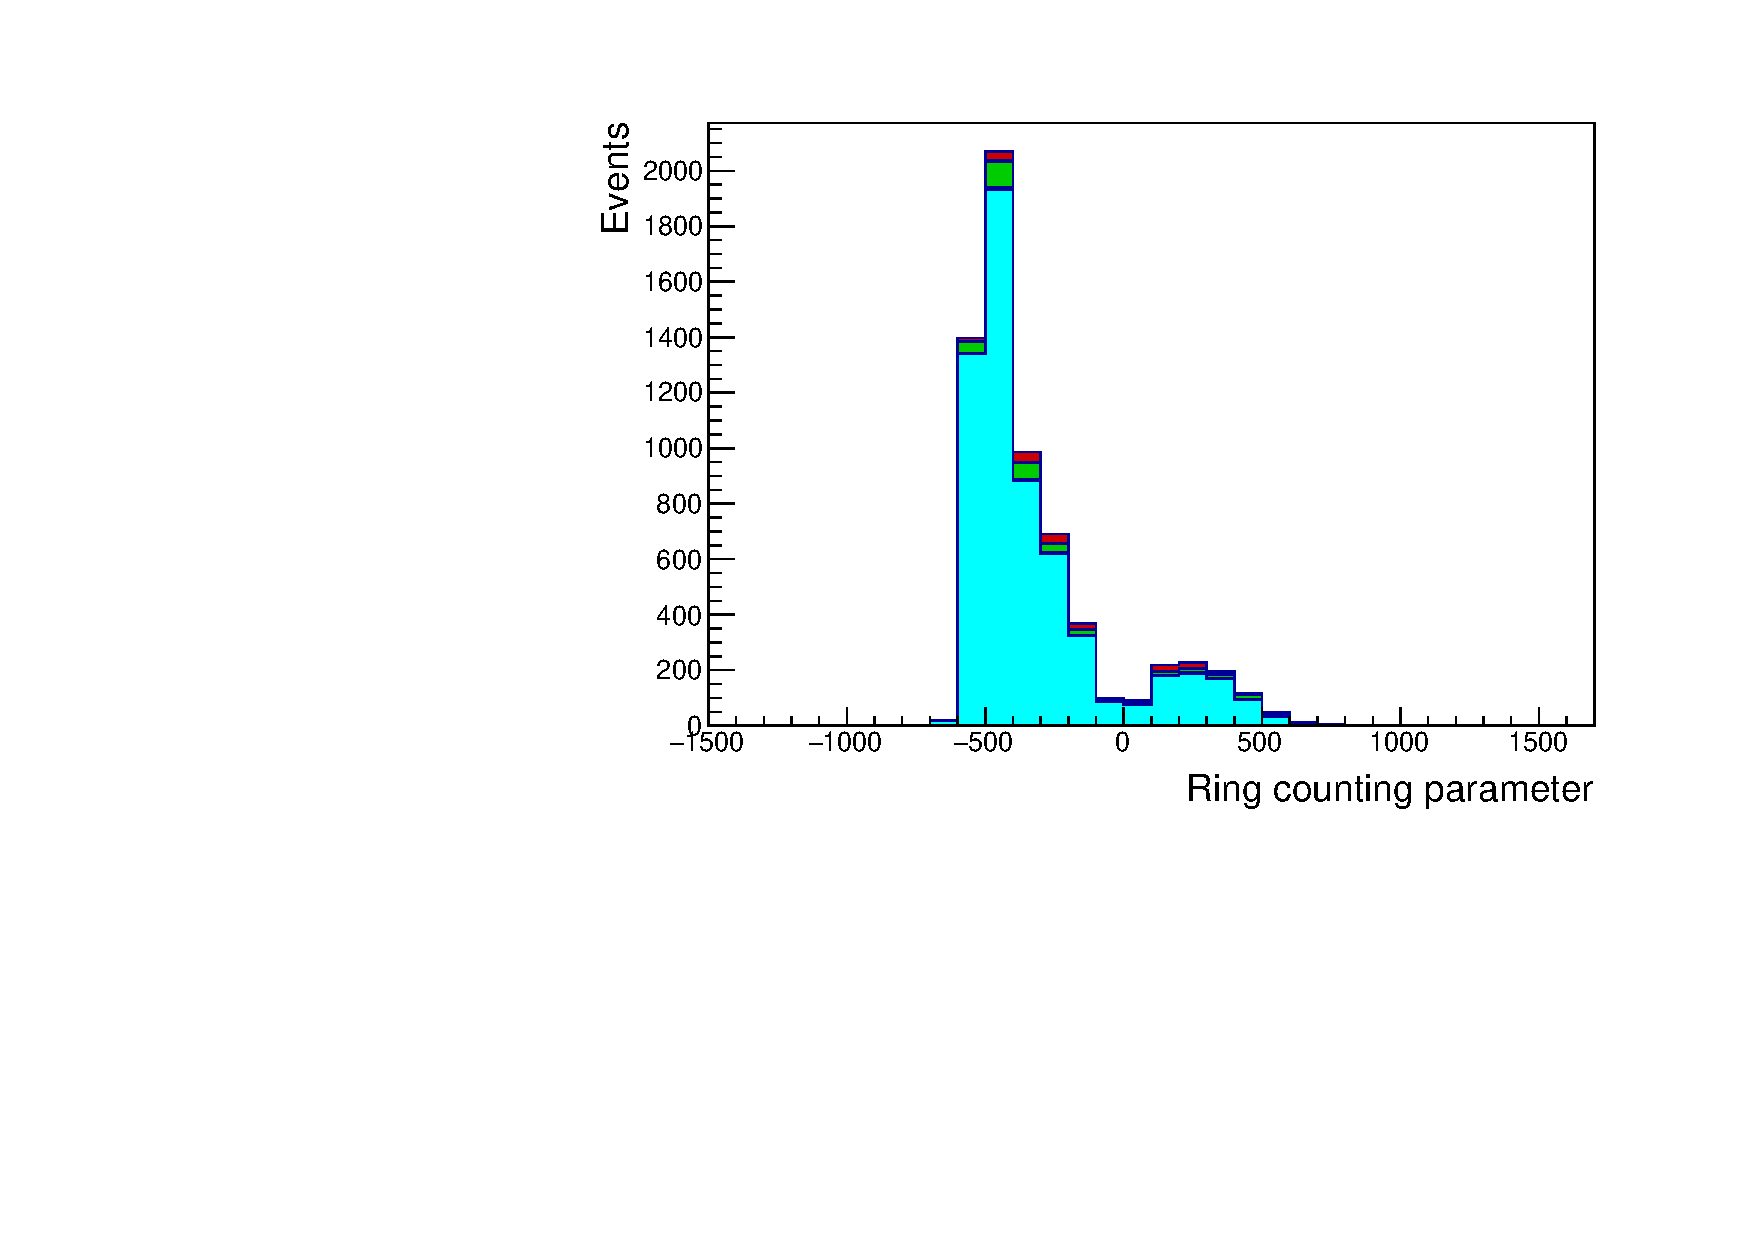
\includegraphics[width=\textwidth, trim={0mm 0mm 0mm 0mm}, clip,page=1]{Figures/Selections/RCParam_SGE0Dcy.pdf}
    \subcaption{\texttt{SubGeV-elike-0dcy}}
  \end{subfigure}%
  \begin{subfigure}[t]{0.49\textwidth}
    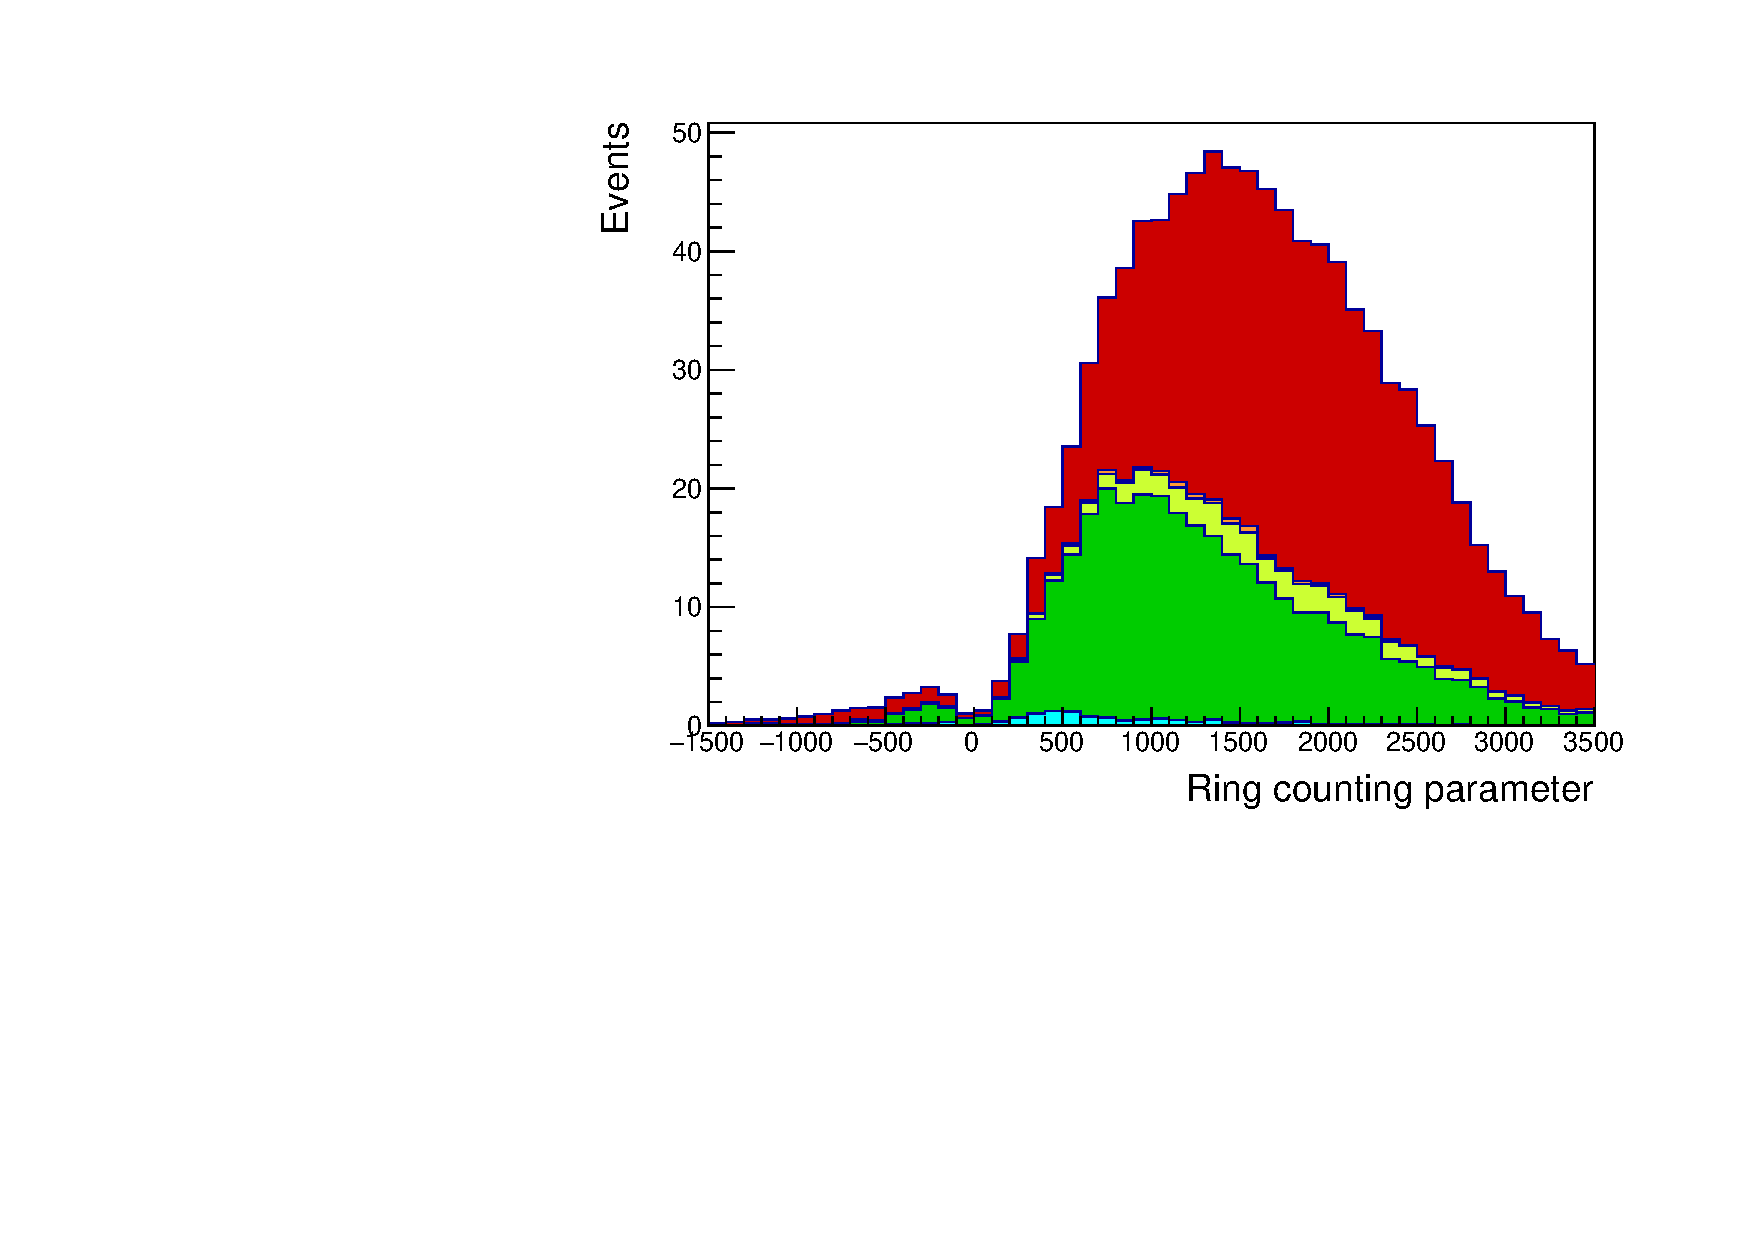
\includegraphics[width=\textwidth, trim={0mm 0mm 0mm 0mm}, clip,page=1]{Figures/Selections/RCParam_MRENue.pdf}
    \subcaption{\texttt{MultiRing-elike-nue}}
  \end{subfigure}
  \begin{subfigure}[t]{0.49\textwidth}
    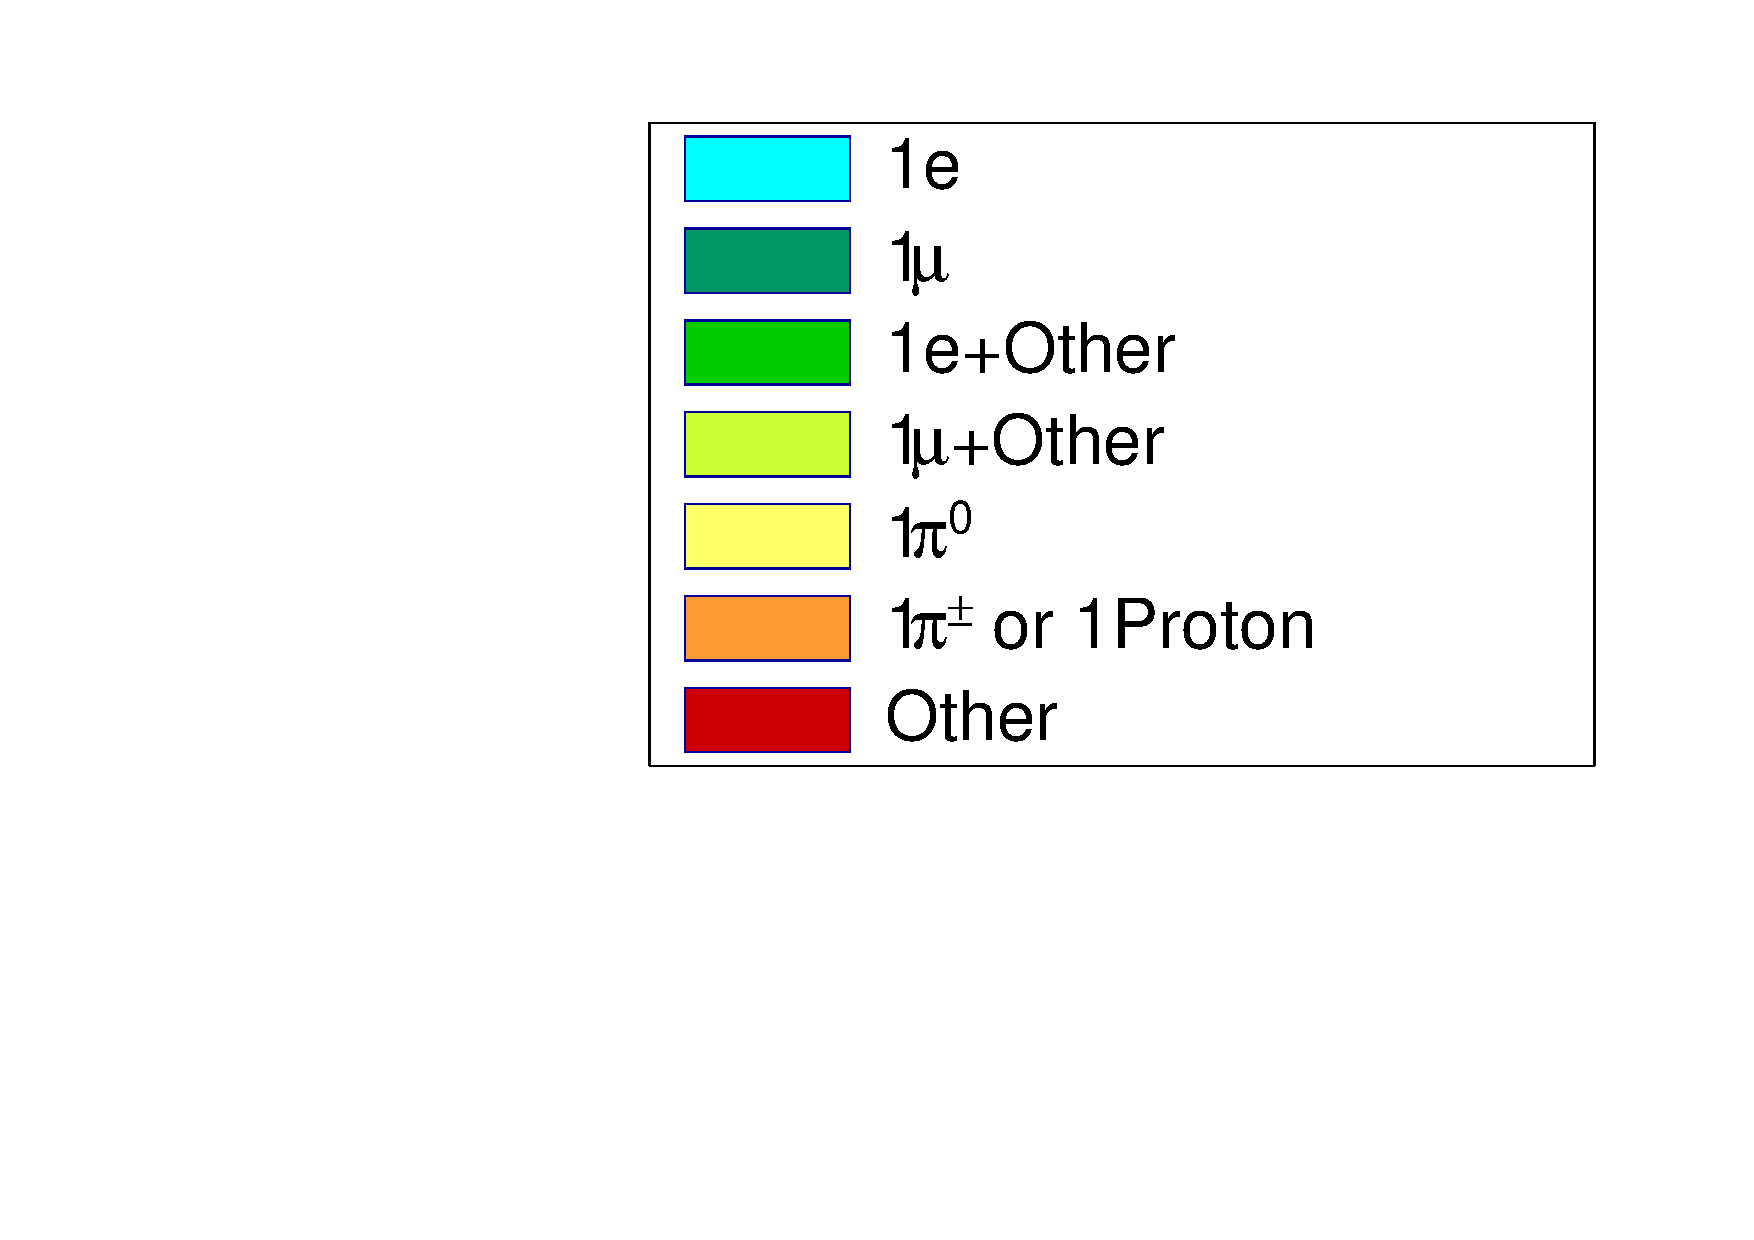
\includegraphics[width=\textwidth, trim={0mm 0mm 0mm 0mm}, clip,page=1]{Figures/Selections/RCParameterLegend.pdf}
  \end{subfigure}
  \caption{The ring counting parameter as defined in \autoref{eqn:SelsAndSysts_Systs_RCParam} for the \texttt{SubGeV-elike-0dcy} and \texttt{MultiRing-elike-nue} samples.}
  \label{fig:SelsAndSysts_RCParameterDistribution}
\end{figure}

As the \texttt{fiTQun} algorithm does not provide a likelihood value after the fake-ring algorithms have been applied, the ring counting parameter distribution is correlated to the final number of reconstructed rings through ``maps''. These are two-dimensional distributions of the ring counting parameter and the final number of reconstructed rings. An example is illustrated in \autoref{fig:SelsAndSysts_RCMaps}. In principle, the \texttt{fiTQun} reconstruction algorithm should be re-run after the variation in the ring counting parameter. However, this is not computationally viable. Therefore the ``maps'' are used as a reweighting template.

The maps are split by final state topology and true neutrino flavour and all \texttt{fiTQun}-reconstructed Monte Carlo events are used to fill them. The maps are row-normalised to represent the probability of \quickmath{X} rings for a given \quickmath{RC_{i}} value. Prior to the oscillation fit, an event's nominal weight is calculated as \quickmath{W^{i}(N^{i}_{Rings},L^{i}_{jk})}, where \quickmath{N^{i}_{Rings}} is the reconstructed number of rings for the \quickmath{i^{th}} event and \quickmath{W^{i}(x,y)} is the bin content in map associated with the \quickmath{i^{th}} event, where \quickmath{x} number of rings and \quickmath{y} is ring counting parameter. Then during the fit, the value of \quickmath{R = W^{i}(N^{i}_{Rings},\bar{L}^{i}_{jk})/W^{i}(N^{i}_{Rings},L^{i}_{jk})} is calculated as the event weight for the \quickmath{i^{th}} event. This is the only cut variable that uses a reweighting technique rather than event migration.

\begin{figure}[h]
  \begin{subfigure}[t]{0.49\textwidth}
    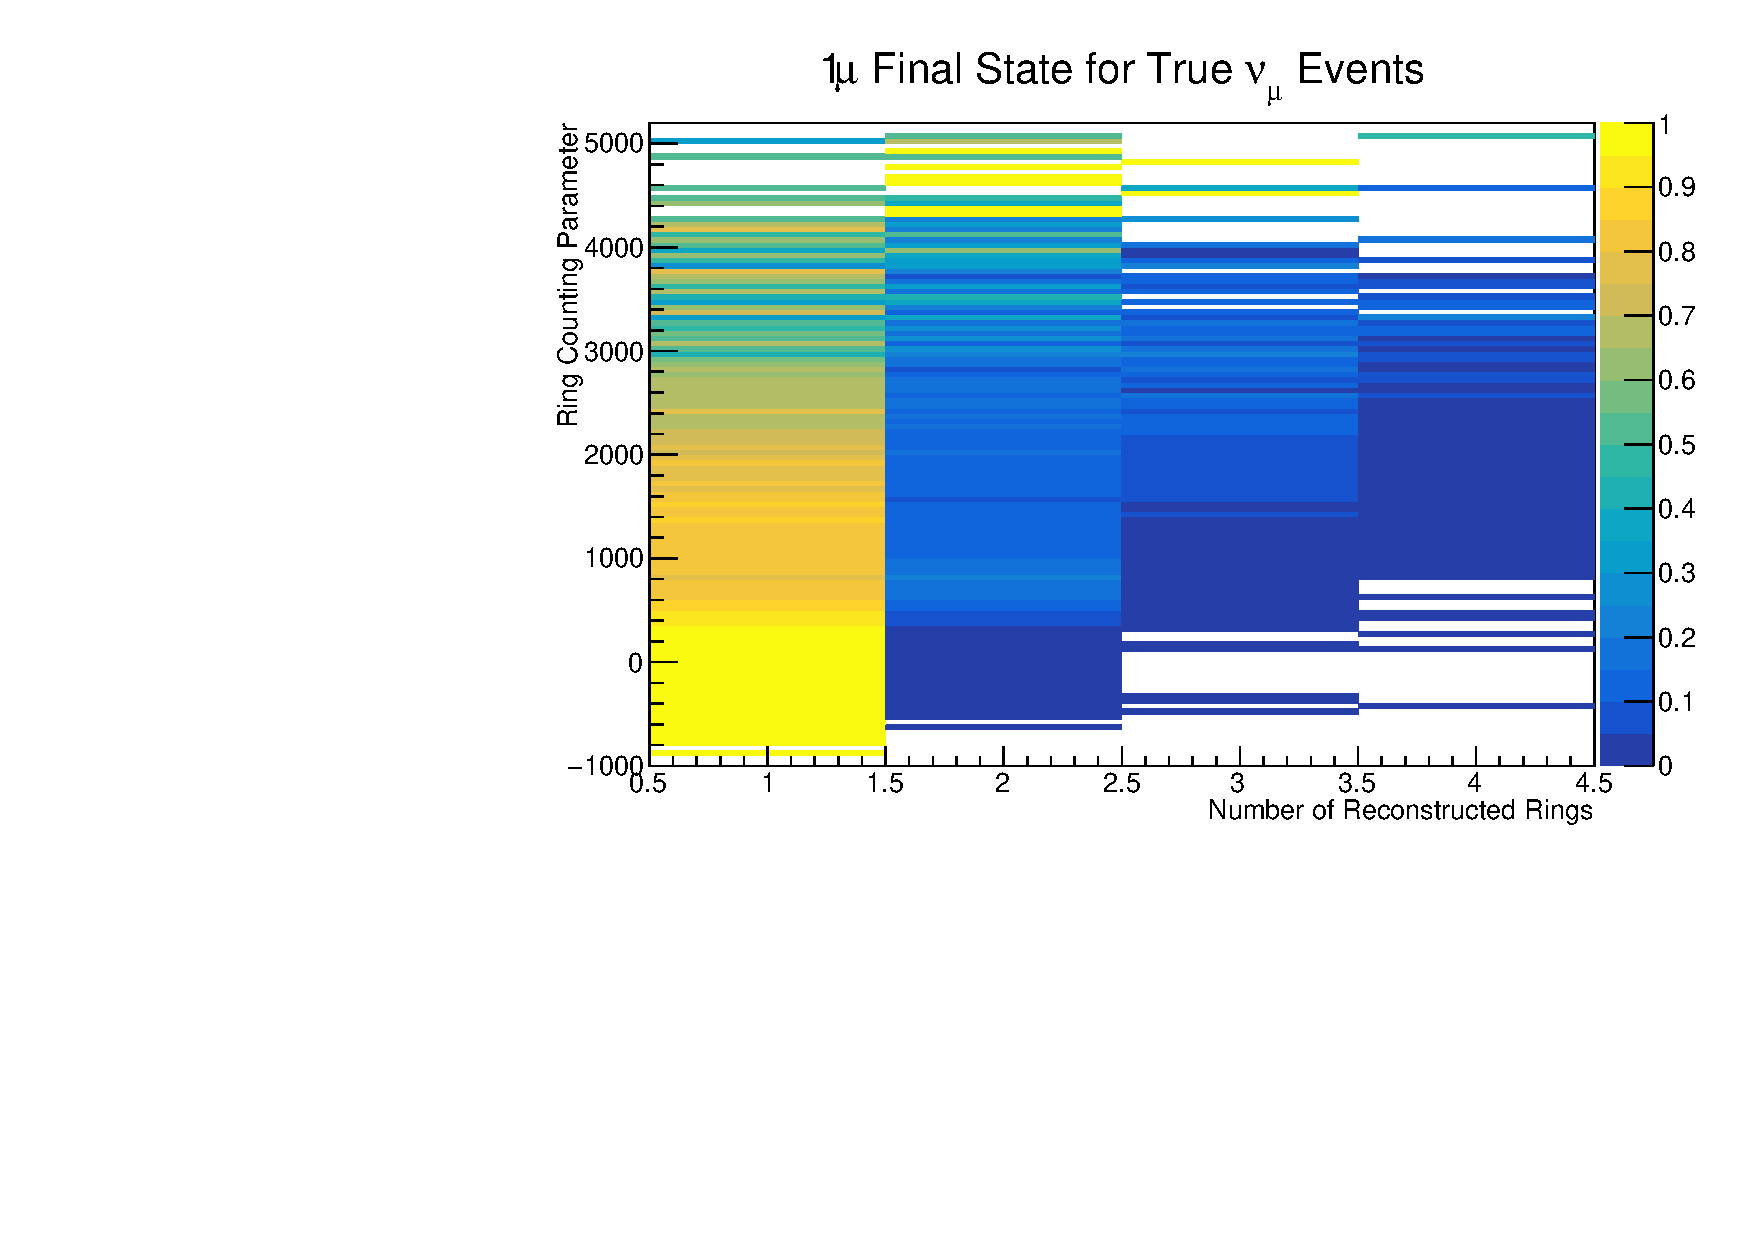
\includegraphics[width=\textwidth, trim={0mm 0mm 0mm 0mm}, clip,page=1]{Figures/Selections/NuFlavour_14_Top_1.pdf}
  \end{subfigure}%
  \begin{subfigure}[t]{0.49\textwidth}
    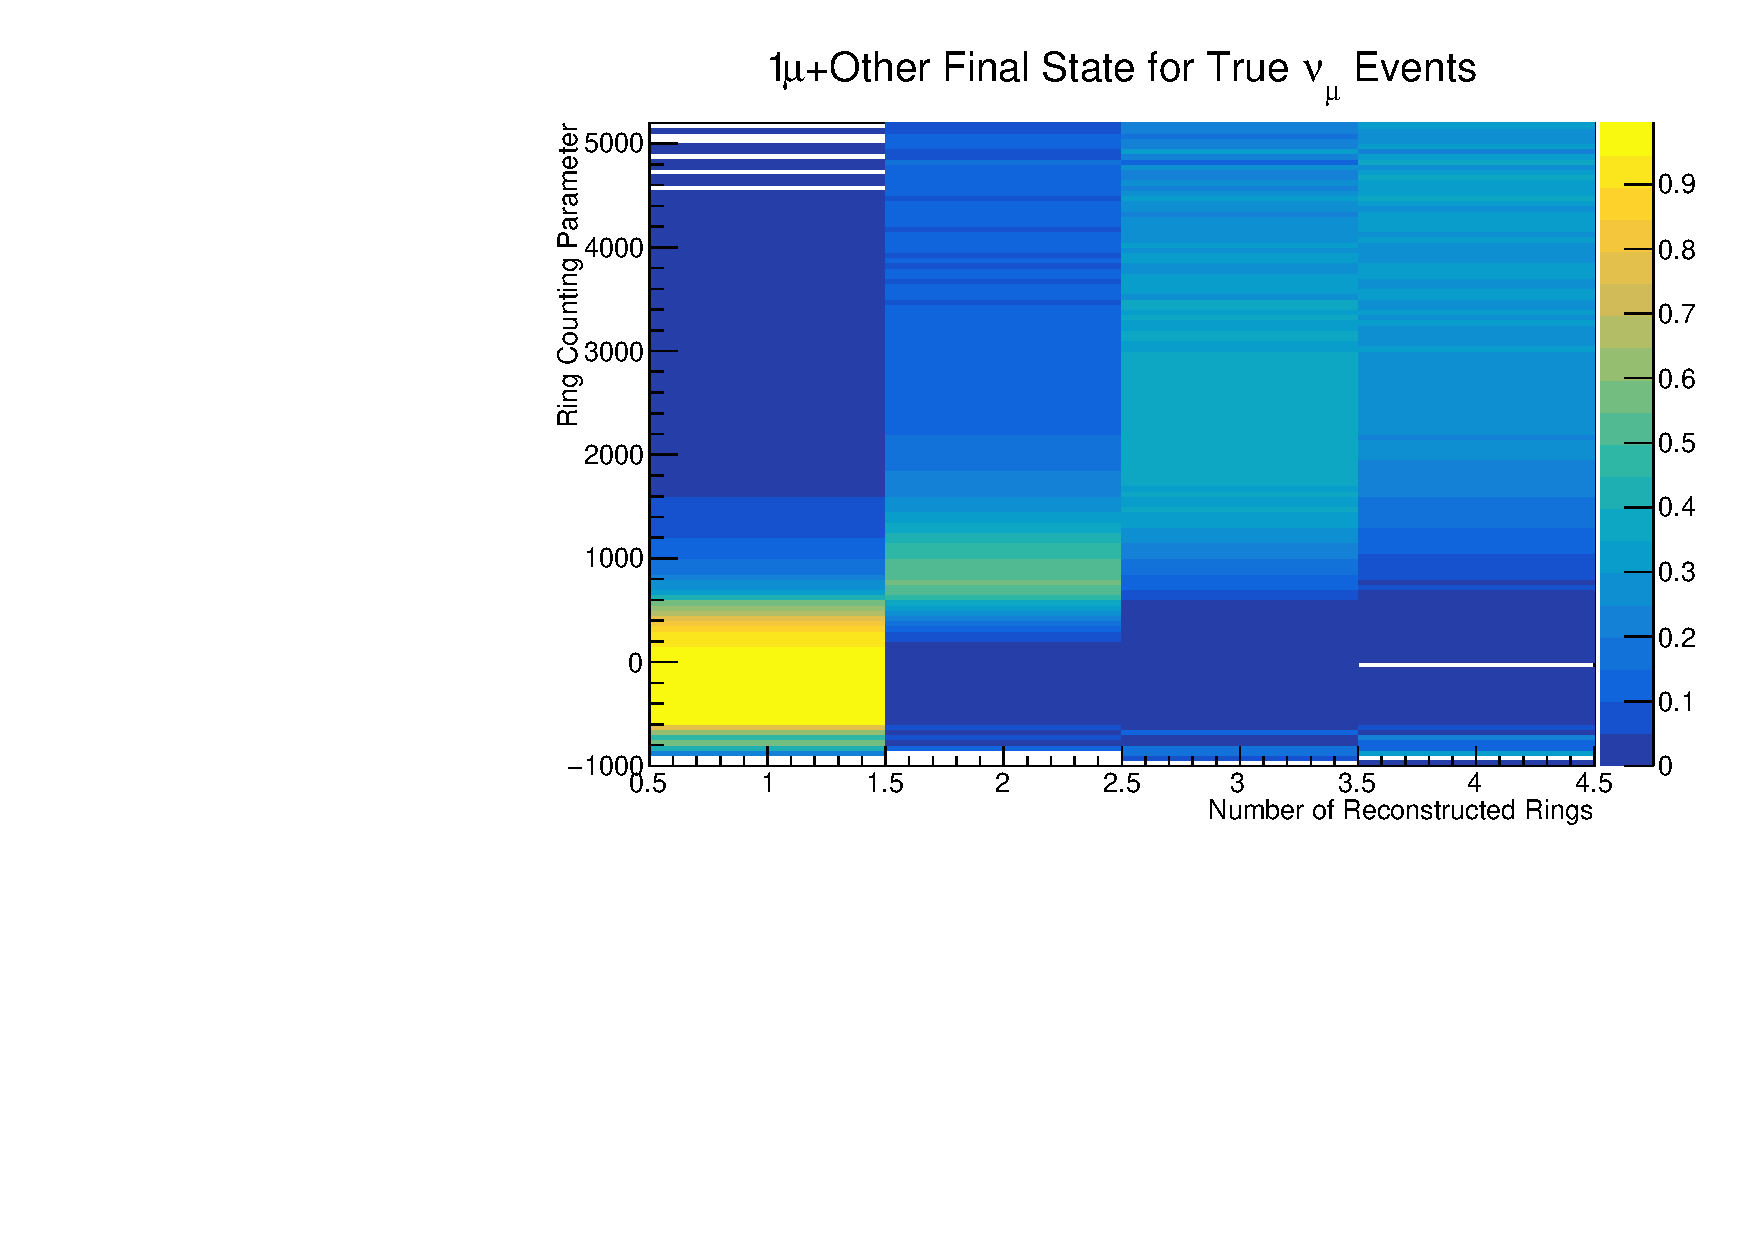
\includegraphics[width=\textwidth, trim={0mm 0mm 0mm 0mm}, clip,page=1]{Figures/Selections/NuFlavour_14_Top_3.pdf}
  \end{subfigure}
  \caption{The ring counting parameter, defined in \autoref{eqn:SelsAndSysts_Systs_RCParam}, as a function of the number of reconstructed rings as found by the \texttt{fiTQun} reconstruction algorithm. Left: true \quickmath{\nu_{\mu}} events with only one muon above the Cherenkov threshold in the final state. Right: true \quickmath{\nu_{\mu}} events with one muon and at least one other charged particle above the Cherenkov threshold in the final state.}
  \label{fig:SelsAndSysts_RCMaps}
\end{figure}

The \quickmath{\pi^{0}} systematics introduced in \autoref{sec:SelsAndSysts_Systs_ND} are applied via a covariance matrix. This is not possible in the alternative model as no covariance matrix is used. Thus, the implementation of the \quickmath{\pi^{0}} systematics has been modified. The inputs from the hybrid \quickmath{\pi^{0}} sample are included via the use of ``\quickmath{\chi^{2}} maps'', which are two-dimensional histograms in \quickmath{\alpha^{i}_{jk}} and \quickmath{\beta^{i}_{jk}} parameters over some range. Illustrative examples of the \quickmath{\chi^{2}} maps are given in \autoref{fig:SelsAndSysts_HybridChi2Maps}. Due to their nature, the shift and smear parameters are typically very correlated. A map is produced for each cut parameter given in \autoref{tab:SelsAndSysts_Systs_CutVariables} and for each visible energy bin given in \autoref{tab:SelsAndSysts_Systs_EVisBinning}.

The maps are filled through the \quickmath{\chi^{2}} comparison of the hybrid \quickmath{\pi^{0}} Monte Carlo and data in the particle identification parameters documented in \autoref{tab:SelsAndSysts_Systs_CutVariables}. The Monte Carlo distribution is modified by the \quickmath{\alpha^{i}_{jk}} and \quickmath{\beta^{i}_{jk}} scaling, whilst cross-section and flux nuisance parameters are thrown from their prior uncertainties. The \quickmath{\chi^{2}} between the scaled Monte Carlo and data is calculated and the relevant point in the \quickmath{\chi^{2}} map is filled.

The implementation within this alternative detector model is to add the bin contents of the maps, for the relevant values of the \quickmath{\alpha^{i}_{jk}} and \quickmath{\beta^{i}_{jk}} parameters, to the likelihood penalty. Only \quickmath{1\pi^{0}} final state topology shift and smear parameters use this prior uncertainty. 

\begin{figure}[h]
  \begin{subfigure}[t]{0.49\textwidth}
    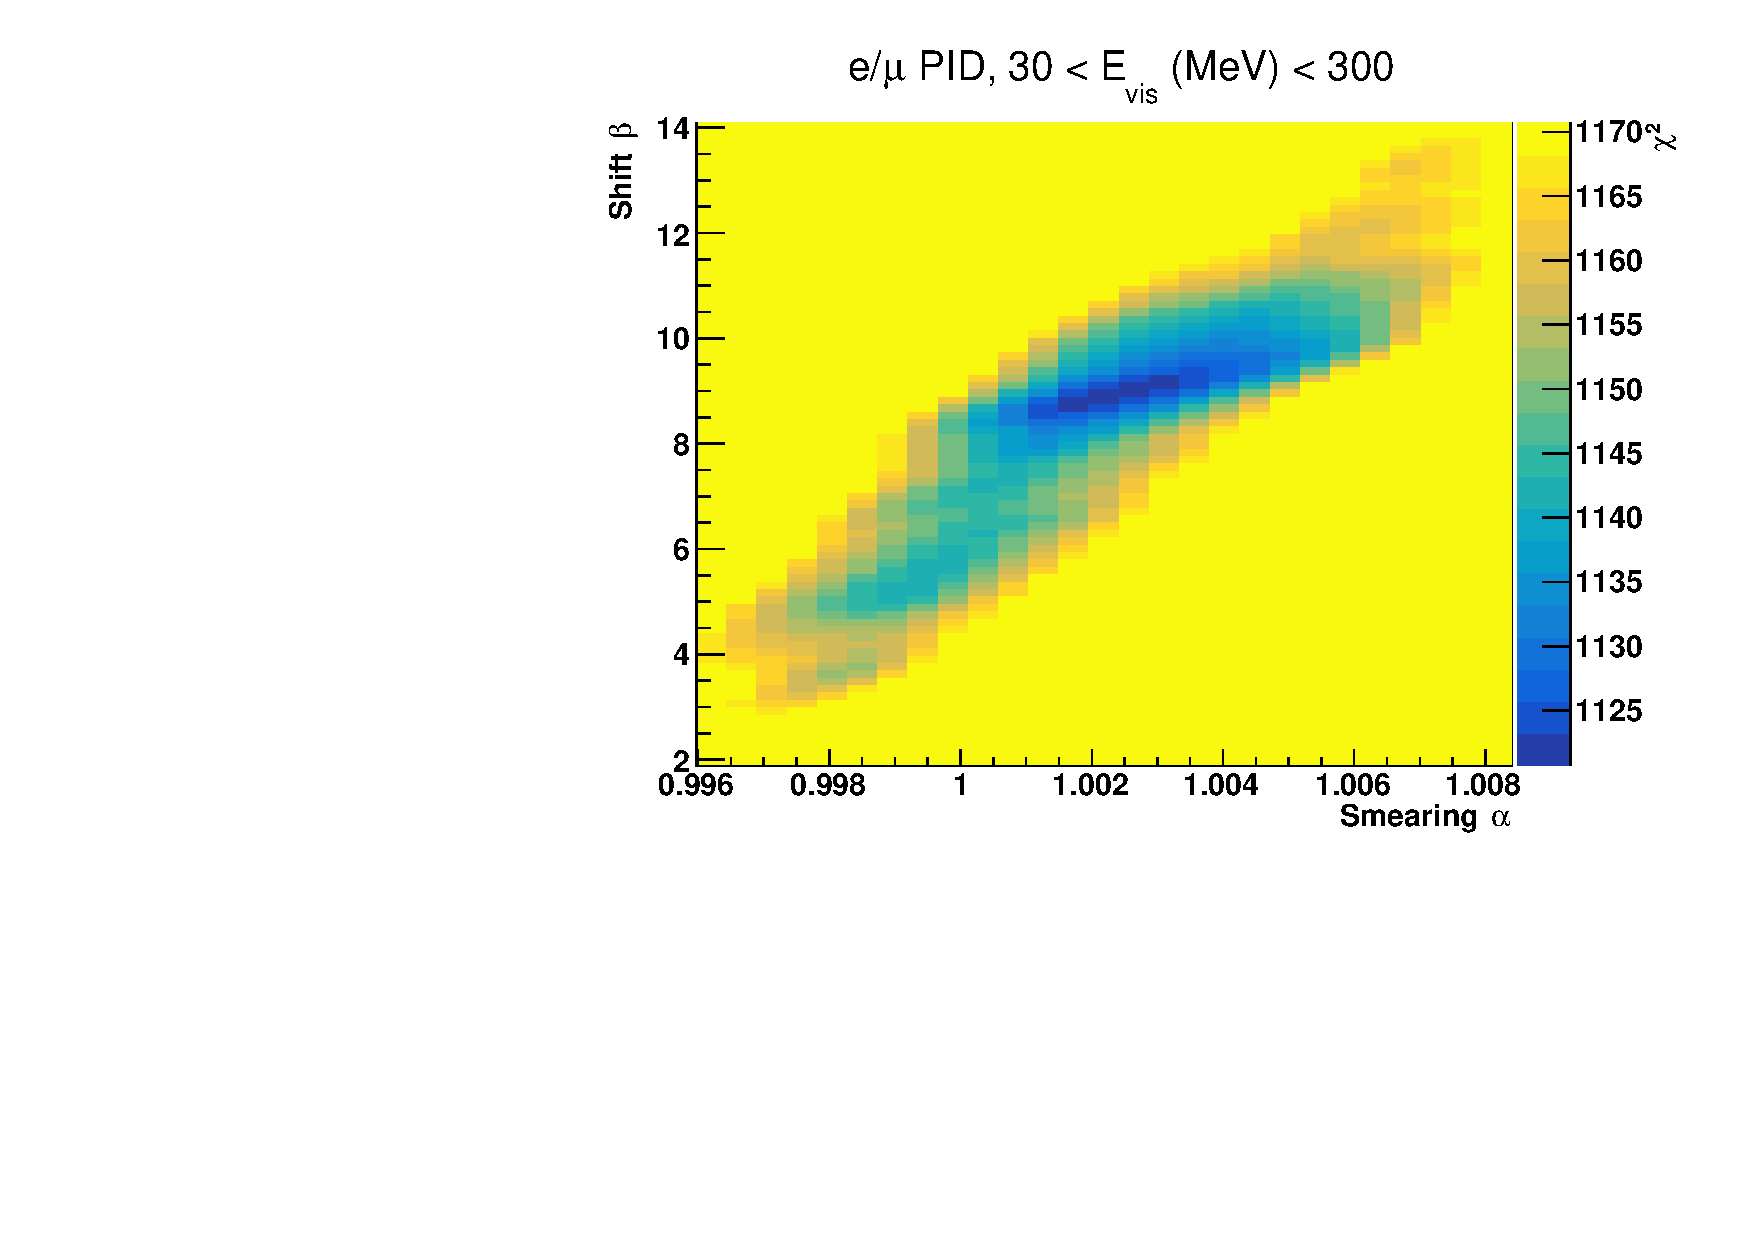
\includegraphics[width=\textwidth, trim={0mm 0mm 0mm 0mm}, clip,page=1]{Figures/Selections/EMUPID_Elt300_Chi2Map.pdf}
  \end{subfigure}%
  \begin{subfigure}[t]{0.49\textwidth}
    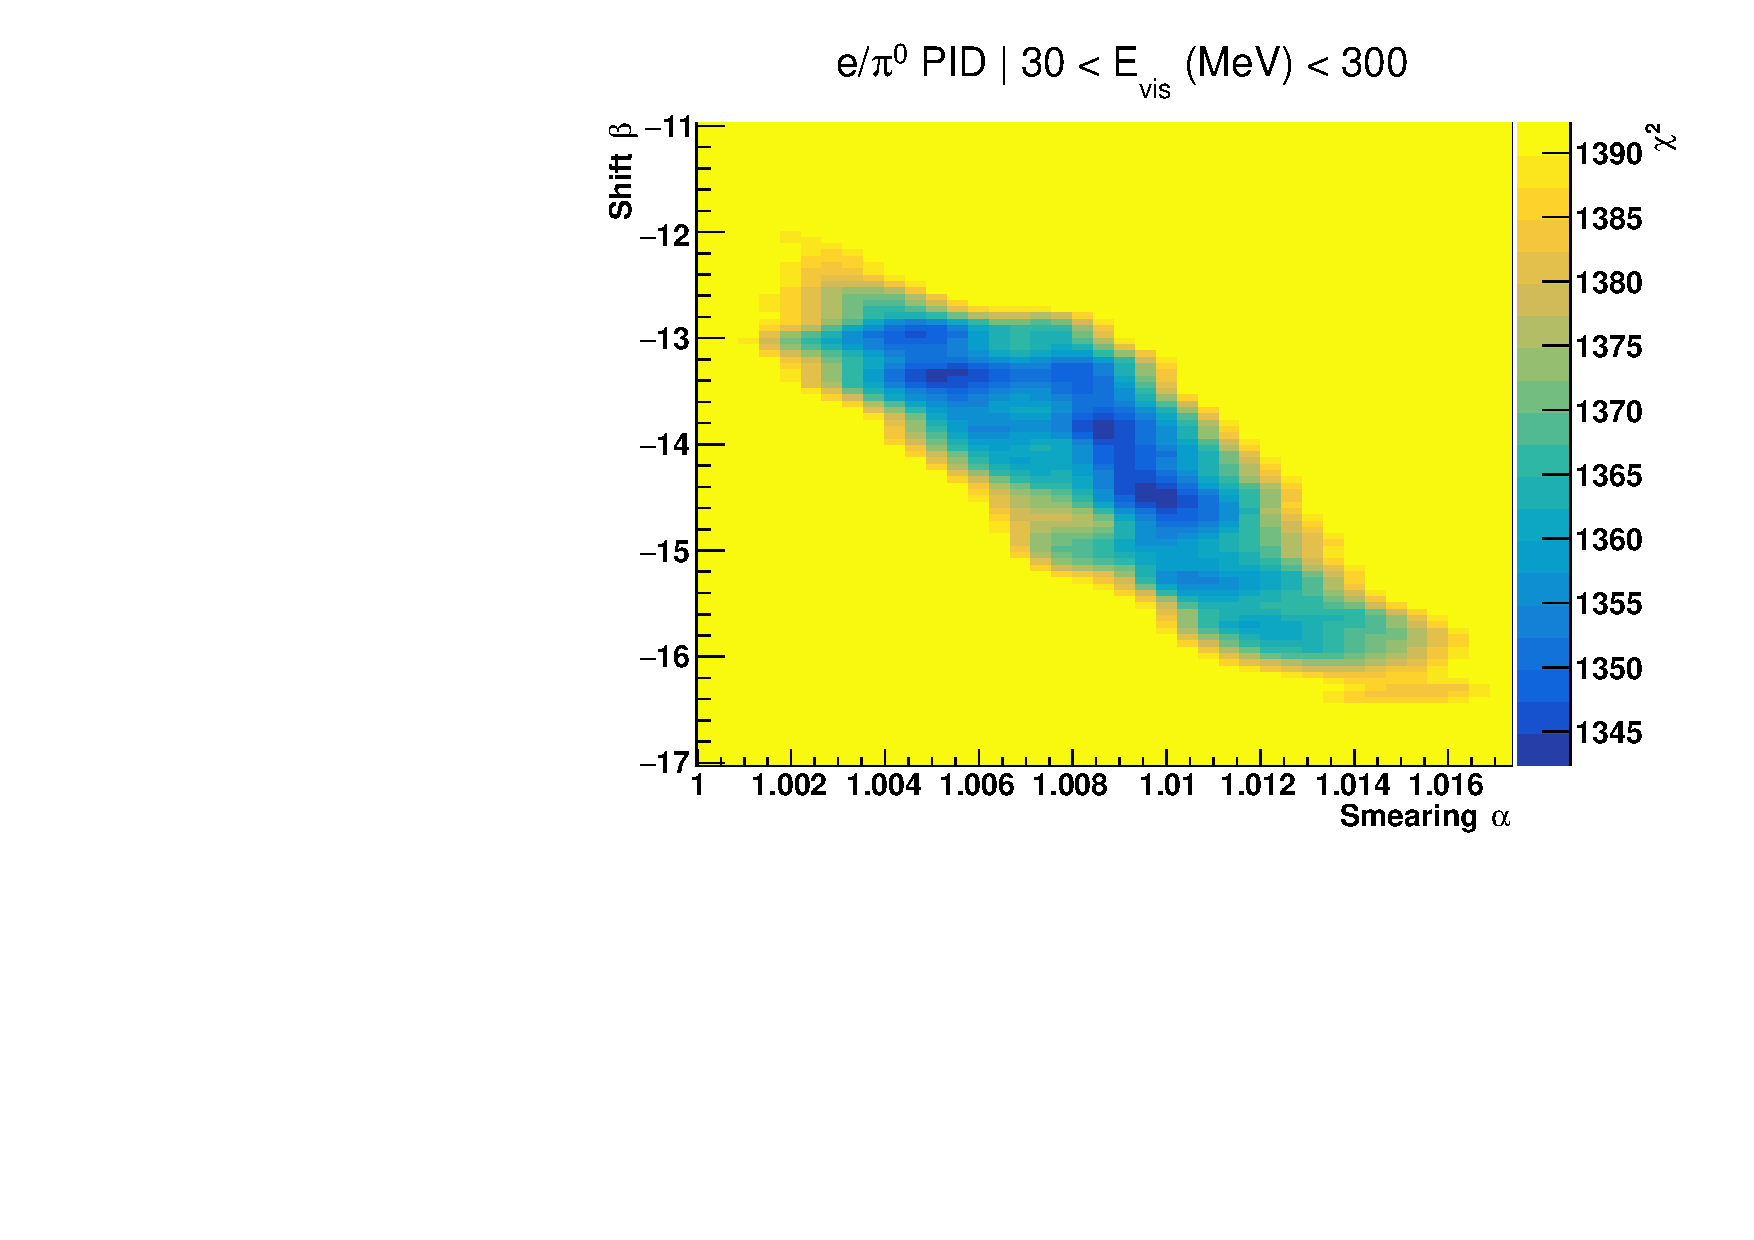
\includegraphics[width=\textwidth, trim={0mm 0mm 0mm 0mm}, clip,page=1]{Figures/Selections/EPI0PID_Elt300_Chi2Map.pdf}
  \end{subfigure}
  \caption{The \quickmath{\chi^{2}} between the hybrid-\quickmath{\pi^{0}} Monte Carlo and data samples, as a function of smear (\quickmath{\alpha}) and shift (\quickmath{\beta}) parameters, for events which have \quickmath{1\pi^{0}} final state topology. Left: Electron-muon separation PID parameter for events with \quickmath{30 \leq E_{vis} (MeV) < 300}. Right: Electron-\quickmath{\pi^{0}} separation PID parameter for events with \quickmath{30 \leq E_{vis} (MeV) < 300}.}
  \label{fig:SelsAndSysts_HybridChi2Maps}
\end{figure}

Similarly, the implementation of the supplementary systematics documented in \autoref{sec:SelsAndSysts_Systs_FDBeam} needs to be modified. A new framework \cite{t2ksk-common} was built in tandem with the T2K-SK working group \cite{t2k_tn_399} so the additional parameters can be incorporated into the MaCh3 framework. These are applied as normalisation parameters, depending on the particular interaction mode, number of tagged decay electrons, and whether the primary particle generated Cherenkov light. They are assigned Gaussian uncertainties with widths described by a covariance matrix. Furthermore, the secondary interaction and photo-nuclear effects need to be accounted for in this detector model using a different implementation than that in \autoref{sec:SelsAndSysts_Systs_FDBeam}. This was done by including a shape parameter for of each of the secondary interactions and the photo-nuclear systematic parameters.

There are a total of \quickmath{224} \quickmath{\alpha^{i}_{jk}} and \quickmath{\beta^{i}_{jk}} parameters, of which \quickmath{32} have prior constraints from the hybrid \quickmath{\pi^0} samples.

One final complexity of this correlated detector model is that the two sets of samples, beam and subGeV atmospheric, use slightly different parameters to distinguish electron and muon-like events. The T2K samples use the value of \quickmath{\log(L_{e}/L_{\mu})} whereas the atmospheric samples use the value of \quickmath{\log(L_{e}/L_{\pi})}, where \quickmath{L_{X}} is the likelihood for hypothesis \quickmath{X}. This is because the T2K fits use single-ring \texttt{fiTQun} fitting techniques, whereas multi-ring fits are applied to the atmospheric samples where only the electron and pion hypothesis are considered. The correlation between the two likelihood ratios is illustrated in \autoref{fig:SelsAndSysts_LLHCorrelation}. As discussed in \autoref{sec:Simulation_Reconstruction}, the pion hypothesis is a very good approximation of the muon hypothesis due to their similar mass. Consequently, using the same shift and smear parameters correlated between the beam and subGeV atmospheric samples is deemed a good approximation.

\begin{figure}[h]
  \begin{subfigure}[t]{0.49\textwidth}
    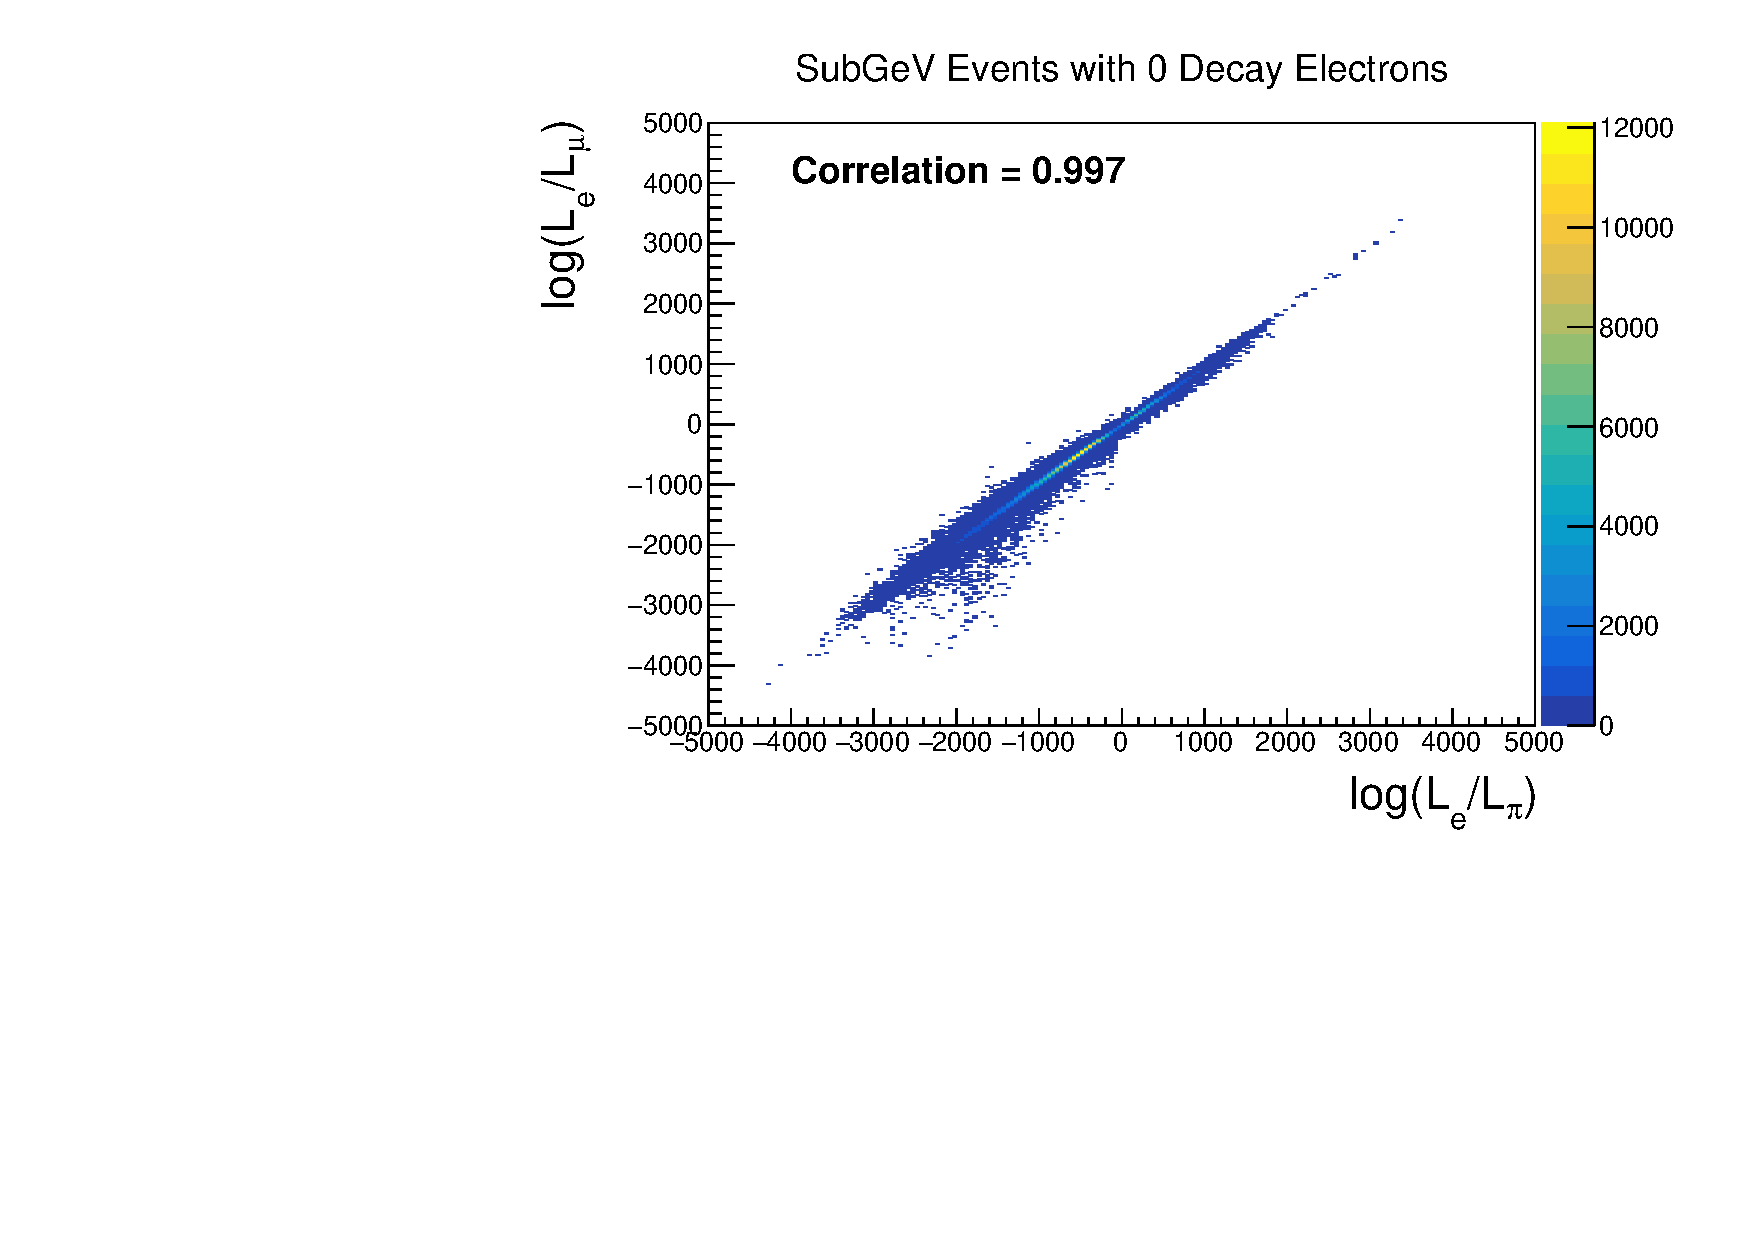
\includegraphics[width=\textwidth, trim={0mm 0mm 0mm 0mm}, clip,page=1]{Figures/Selections/Correlation_SG0Dcy.pdf}
  \end{subfigure}%
  \begin{subfigure}[t]{0.49\textwidth}
    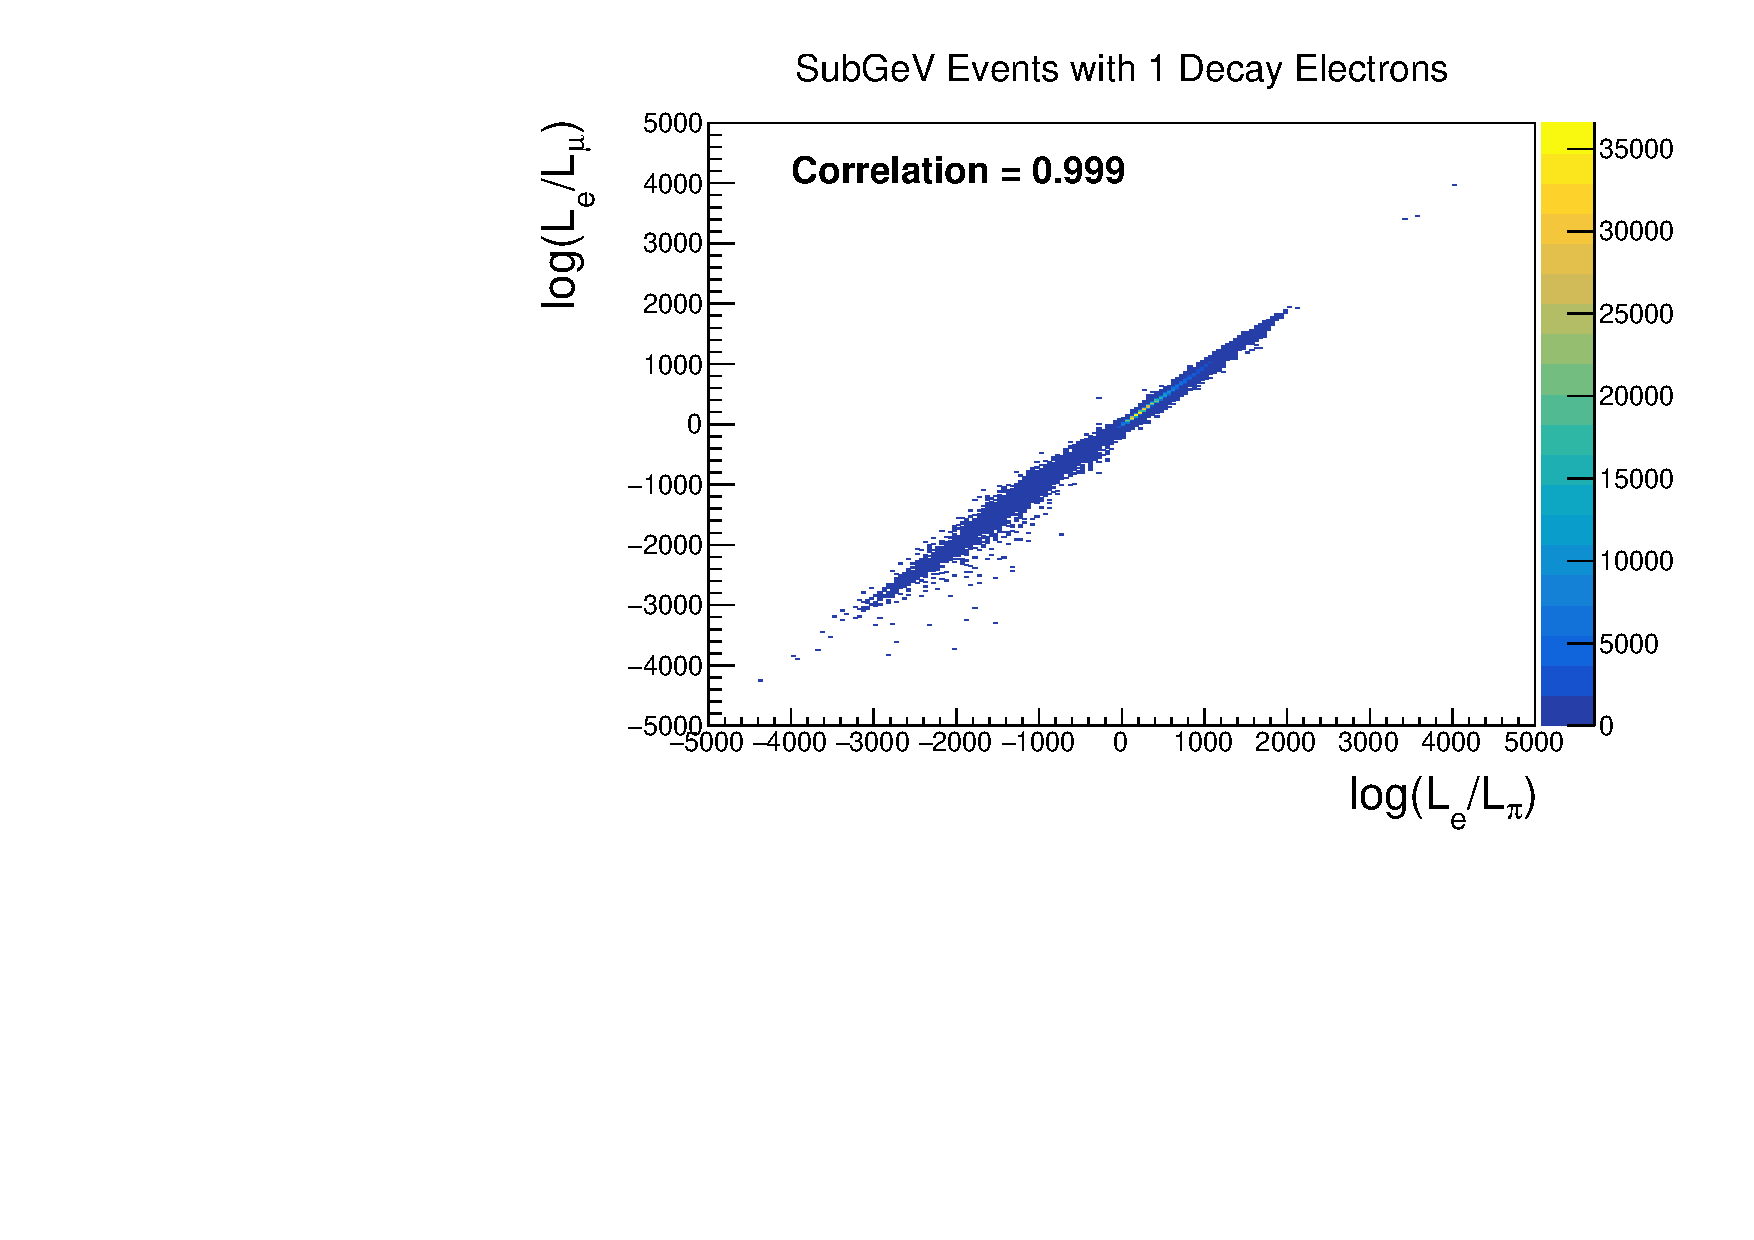
\includegraphics[width=\textwidth, trim={0mm 0mm 0mm 0mm}, clip,page=1]{Figures/Selections/Correlation_SG1Dcy.pdf}
  \end{subfigure}
  \begin{subfigure}[t]{0.49\textwidth}
    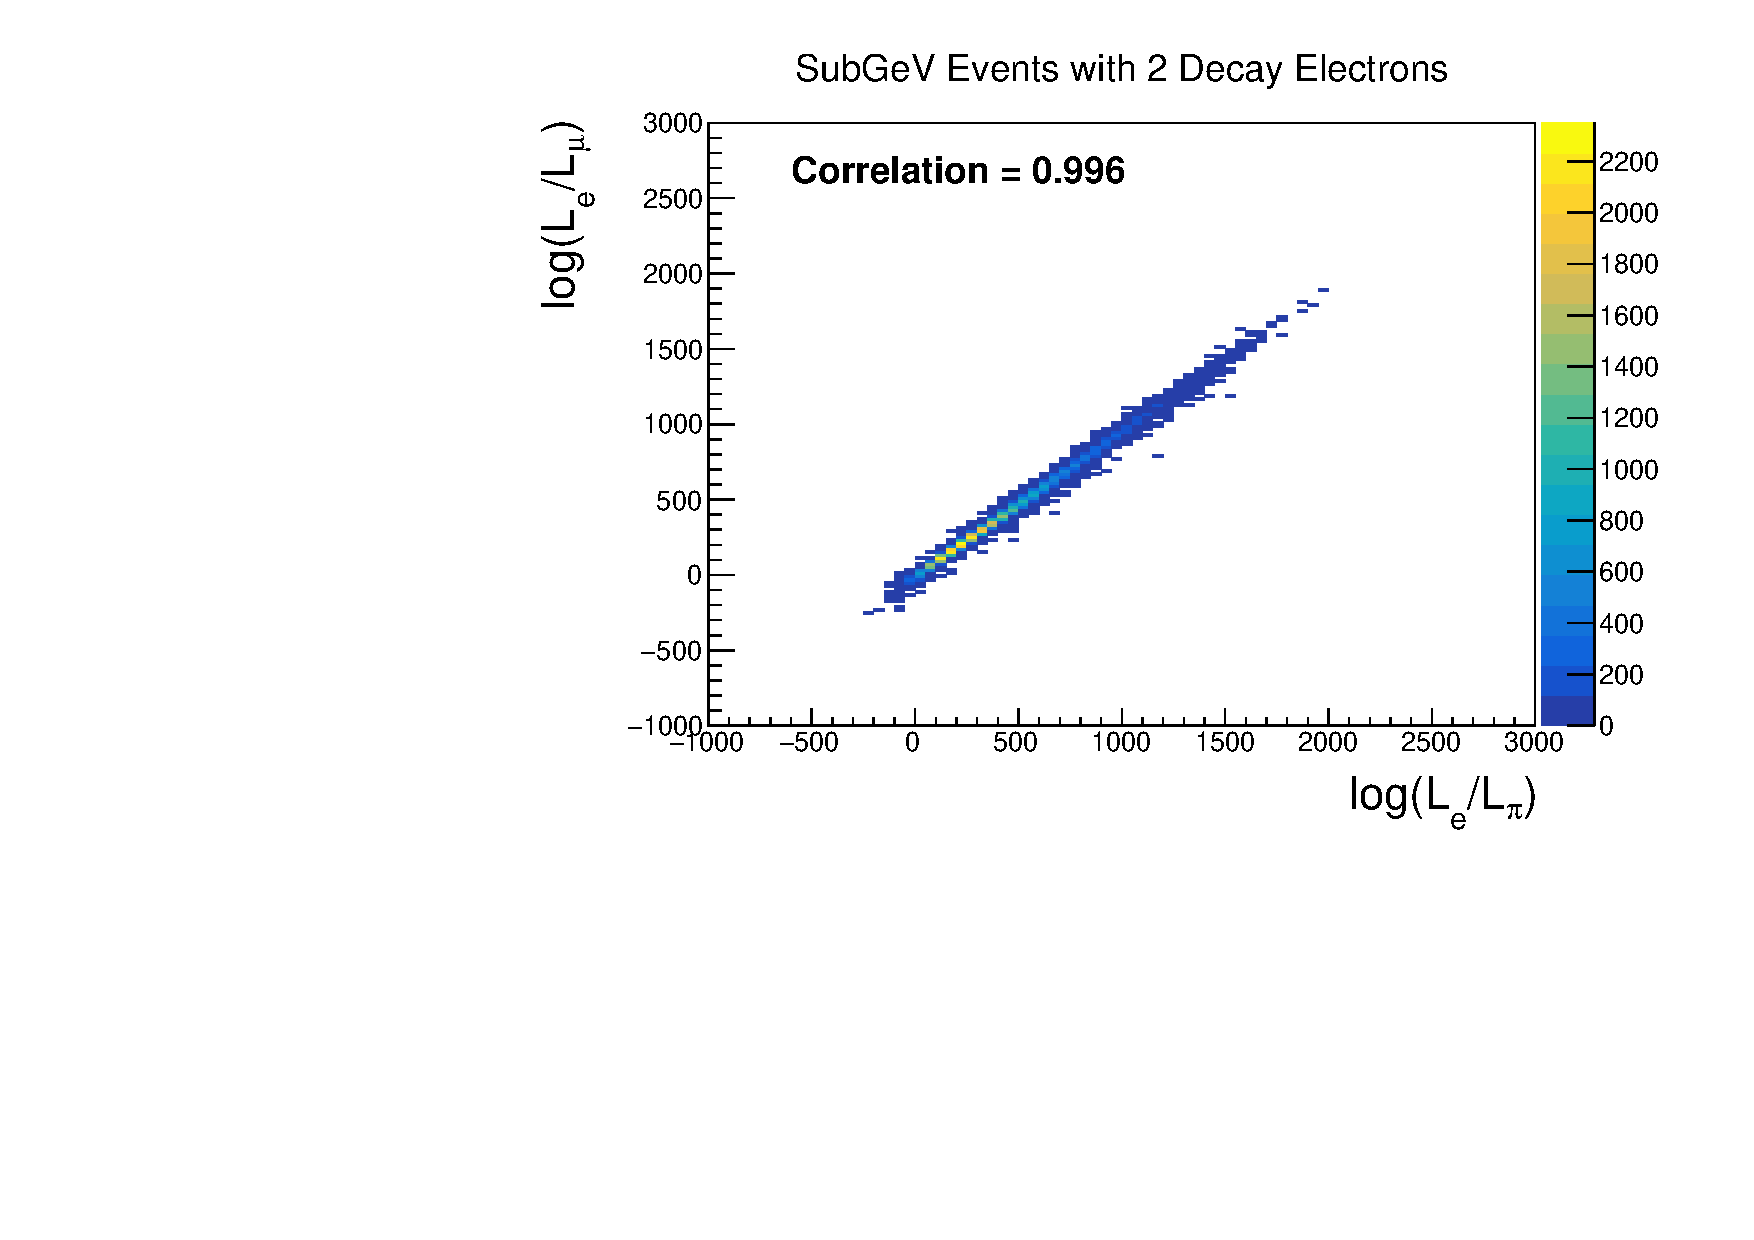
\includegraphics[width=\textwidth, trim={0mm 0mm 0mm 0mm}, clip,page=1]{Figures/Selections/Correlation_SG2Dcy.pdf}
  \end{subfigure}
  \caption{The distribution of \quickmath{\log(L_{e}/L_{\mu})} compared to \quickmath{\log(L_{e}/L_{\pi})} for subGeV events with zero (top left), one (top right) or two (bottom) decay electrons. The correlation in the distribution is calculated as \quickmath{0.997}, \quickmath{0.999} and \quickmath{0.996}, respectively.}
  \label{fig:SelsAndSysts_LLHCorrelation}
\end{figure}

\section{Likelihood Calculation}
\label{sec:OscillationAnalysis_LLHCalc}

This analysis performs a joint oscillation parameter fit of the ND280 beam samples, the T2K far detector beam samples, and the SK atmospheric samples introduced in this chapter. 

Once the Monte Carlo predictions of each beam and atmospheric sample have been built, a likelihood needs to be constructed. This is done by comparing the binned Monte Carlo prediction to binned data. The Monte Carlo prediction is calculated at a particular point, \quickmath{\vec{\theta}}, in the model parameter space such that \quickmath{N_{i}^{MC} = N_{i}^{MC}(\vec{\theta})}, where \quickmath{N_{i}} represents the bin content of the \quickmath{i^{th}} bin. The data and Monte Carlo spectra are represented by \quickmath{N_{i}^{D}} and \quickmath{N_{i}^{MC}}, respectively. The bin contents for the beam near detector, beam far detector and atmospheric samples are denoted with \quickmath{ND}, \quickmath{FD}, and \quickmath{Atm}, respectively. The binning index, \quickmath{i}, runs over all the bins within a sample. Taking the \texttt{FHC1Rmu} far detector sample as an example, the binning index runs over all the reconstructed neutrino energy bins. The likelihood calculation between the data and the Monte Carlo prediction for a particular bin follows a Poisson distribution, where the data is treated as a fluctuation of the simulation. 

The data can consist of either real data or an `Asimov' Monte Carlo prediction, which is typically used for sensitivity studies and denoted `Asimov data'. The process for building Asimov data is as follows. The Monte Carlo prediction is reweighted using a particular set of oscillation parameters (potentially those listed in \autoref{tab:Theory_ParameterSets}) and systematic parameter tune. The resulting spectra for each sample is then defined to be the Asimov data for that sample. Whilst this results in unphysical non-integer data predictions, it eliminates statistical fluctuations from the data. Therefore, the results of a fit to Asimov data should not include any biases from statistical fluctuations. Furthermore, these results should produce posterior probability distributions consistent with the parameters which were used to make the data prediction. That is to say, the fit results should return the known parameters. Any biases seen would be attributed to correlations between each oscillation parameter and correlations between oscillation and systematic parameters. Consequently, Asimov fit results present the maximum precision at which the oscillation parameters could be measured to.

Following the T2K analysis presented in \cite{Dunne2020-uf}, the likelihood contribution for the near detector samples also includes a Monte Carlo statistical uncertainty term, derived from the Barlow and Beeston statistical treatment \cite{Barlow1993-cc, Conway2011-go}. In addition to treating the data as a Poisson fluctuation of the Monte Carlo prediction, it includes a contribution to the likelihood that which treats the generated Monte Carlo prediction as a statistical fluctuation of the actual true simulation assuming an infinite amount of statistics had been created. The technical implementation of this additional likelihood term is documented in \cite{t2k_tn_395} and briefly summarised as follows. The term is defined as,

\begin{equation}
  \frac{(\beta_{i}-1)^{2}}{2\sigma^{2}_{\beta_{i}}},
\end{equation}

where \quickmath{\beta_{i}} represents a scaling parameter for the \quickmath{i^{th}} bin that relates the bin content for the amount of Monte Carlo actually generated \quickmath{N^{MC}_{i}} to the bin content if an infinite amount of Monte Carlo statistics had been generated \quickmath{N^{MC}_{i,true}}, such that \quickmath{N^{MC}_{i,true} = \beta_{i} \times N^{MC}_{i}}. In the case where a sufficient amount of Monte Carlo statistics had been generated, \quickmath{\beta_{i} = 1}. An analytical solution for \quickmath{\beta_{i}} is given in \cite{t2k_tn_395}. Additionally, \quickmath{\sigma_{\beta_{i}} = \sqrt{\sum_{i} w_{i}^{2}}/N_{i}^{MC}} where \quickmath{\sqrt{\sum_{i} w_{i}^{2}}} represents the sum of the square of the weights of the Monte Carlo events which fall into bin \quickmath{i}.

An additional contribution to the likelihood comes from the variation of the systematic model parameters. For those parameters with well-motivated uncertainty estimates, a covariance matrix, \quickmath{V}, describes the prior knowledge of each parameter as well as any correlations between the parameters. Due to a technical implementation, a single covariance matrix describes each ``block'' of model parameters, e.g. beam flux systematics. The covariance matrix associated with the \quickmath{k^{th}} block is denoted \quickmath{V^{k}}. This substitution results in \quickmath{\vec{\theta} = \sum_{k}^{N_{b}} \vec{\theta}^{k}} and \quickmath{V = \sum_{k}^{N_{b}} V^{k}} where \quickmath{N_{b}} denotes the number of blocks. A single covariance matrix is provided for: the oscillation parameters, the beam flux parameters, the atmospheric flux parameters, the neutrino interaction systematics, the near detector parameters, the beam far detector systematics, and the atmospheric far detector systematics. The number of parameters in the \quickmath{k^{th}} block is defined as \quickmath{n(k)}.

The equation for the likelihood \quickmath{\mathcal{L}} includes all the terms discussed above. It is defined as,

\iffalse
\begin{align}
\label{eqn:Likelihood:Likelihood}
&-\ln(\mathcal{L}) = \\ 
& \sum_{i}^{\mathsf{ND bins}} N_{i}^{\mathrm{ND},MC}(\vec{\theta}) - N_{i}^{\mathrm{ND},D} + N_{i}^{\mathrm{ND},D}  \times \ln \left[ N_{i}^{\mathrm{ND},D}/N_{i}^{\mathrm{ND},MC}(\vec{\theta}) \right] + \frac{(\beta_{i}-1)^{2}}{2\sigma^{2}_{\beta_{i}}} \nonumber \\
& +  \sum_{i}^{\mathsf{FD bins}} N_{i}^{\mathrm{FD},MC}(\vec{\theta}) - N_{i}^{\mathrm{FD},D} + N_{i}^{\mathrm{FD},D}  \times \ln \left[ N_{i}^{\mathrm{FD},D}/N_{i}^{\mathrm{FD},MC}(\vec{\theta}) \right] \nonumber \\ 
 +  \sum_{i}^{\mathsf{Atm bins}} N_{i}^{\mathrm{Atm},MC}( \vec{\theta}) - N_{i}^{\mathrm{Atm},D} + N_{i}^{\mathrm{Atm},D} \times  \ln \left[ N_{i}^{\mathrm{Atm},D}/N_{i}^{\mathrm{Atm},MC}(\vec{\theta}) \right] \nonumber \\ 
& + \frac{1}{2} \sum_{k}^{N_{b}} \sum_{i}^{n(k)} \sum_{j}^{n(k)} (\vec{\theta}^{k})_{i} (V^{k})^{-1}_{ij} (\vec{\theta}^{k})_{j}. \nonumber
\end{align}
\fi

\begin{equation}
  \label{eqn:Likelihood:Likelihood}
  \begin{split}
    &-\ln(\mathcal{L}) = \\ 
    & \sum_{i}^{\mathsf{ND bins}} N_{i}^{\mathrm{ND},MC}(\vec{\theta}) - N_{i}^{\mathrm{ND},D} + N_{i}^{\mathrm{ND},D}  \times \ln \left[ N_{i}^{\mathrm{ND},D}/N_{i}^{\mathrm{ND},MC}(\vec{\theta}) \right] + \frac{(\beta_{i}-1)^{2}}{2\sigma^{2}_{\beta_{i}}} \\
    & +  \sum_{i}^{\mathsf{FD bins}} N_{i}^{\mathrm{FD},MC}(\vec{\theta}) - N_{i}^{\mathrm{FD},D} + N_{i}^{\mathrm{FD},D}  \times \ln \left[ N_{i}^{\mathrm{FD},D}/N_{i}^{\mathrm{FD},MC}(\vec{\theta}) \right] \\
    & +  \sum_{i}^{\mathsf{Atm bins}} N_{i}^{\mathrm{Atm},MC}( \vec{\theta}) - N_{i}^{\mathrm{Atm},D} + N_{i}^{\mathrm{Atm},D} \times  \ln \left[ N_{i}^{\mathrm{Atm},D}/N_{i}^{\mathrm{Atm},MC}(\vec{\theta}) \right] \\
    & + \frac{1}{2} \sum_{k}^{N_{b}} \sum_{i}^{n(k)} \sum_{j}^{n(k)} (\vec{\theta}^{k})_{i} (V^{k})^{-1}_{ij} (\vec{\theta}^{k})_{j}.
  \end{split}
\end{equation}

The negative log-likelihood value is determined at each step of the MCMC to build the posterior distribution defined in \autoref{chap:MarkovChainMonteCarlo}. This value is minimised when the Monte Carlo prediction tends towards the data spectrum.
